\documentclass[12pt, %
openright, 
oneside, %
%twoside, %TCC: Se seu texto tem mais de 100 páginas, descomente esta linha e comente a anterior
a4paper,    %
%english,   %
brazil]{facom-ufu-abntex2}

\usepackage{graphicx}
\usepackage{tabularx}
\usepackage{subcaption}
\usepackage{float}
\usepackage{amsmath}

\graphicspath{{figuras/}{pictures/}{images/}{./}} % where to search for the images

\newcommand{\blue}[1]{\textcolor{blue}{#1}}
\newcommand{\red}[1]{\textcolor{red}{#1}}


\autor{Henrique Tornelli Duarte} %TCC
\data{2025}
\orientador{Professor Dino Rogerio Coinete Franklin} %TCC


% ---
% Informações de dados para CAPA e FOLHA DE ROSTO
% ---

\titulo{Geração e Aperfeiçoamento de Logotipos via Ajuste Fino no Stable Diffusion XL} %TCC

\hypersetup{pdfkeywords={IA}{deep learning}{geração de imagem}{logotipos}{LoRA}} %TCC

\begin{document}
\frenchspacing 

% ----------------------------------------------------------
% ELEMENTOS PRÉ-TEXTUAIS
% ----------------------------------------------------------
%\pretextual
\imprimircapa
\imprimirfolhaderosto
% ---


% ---
% Inserir folha de aprovação
% ---
%
% 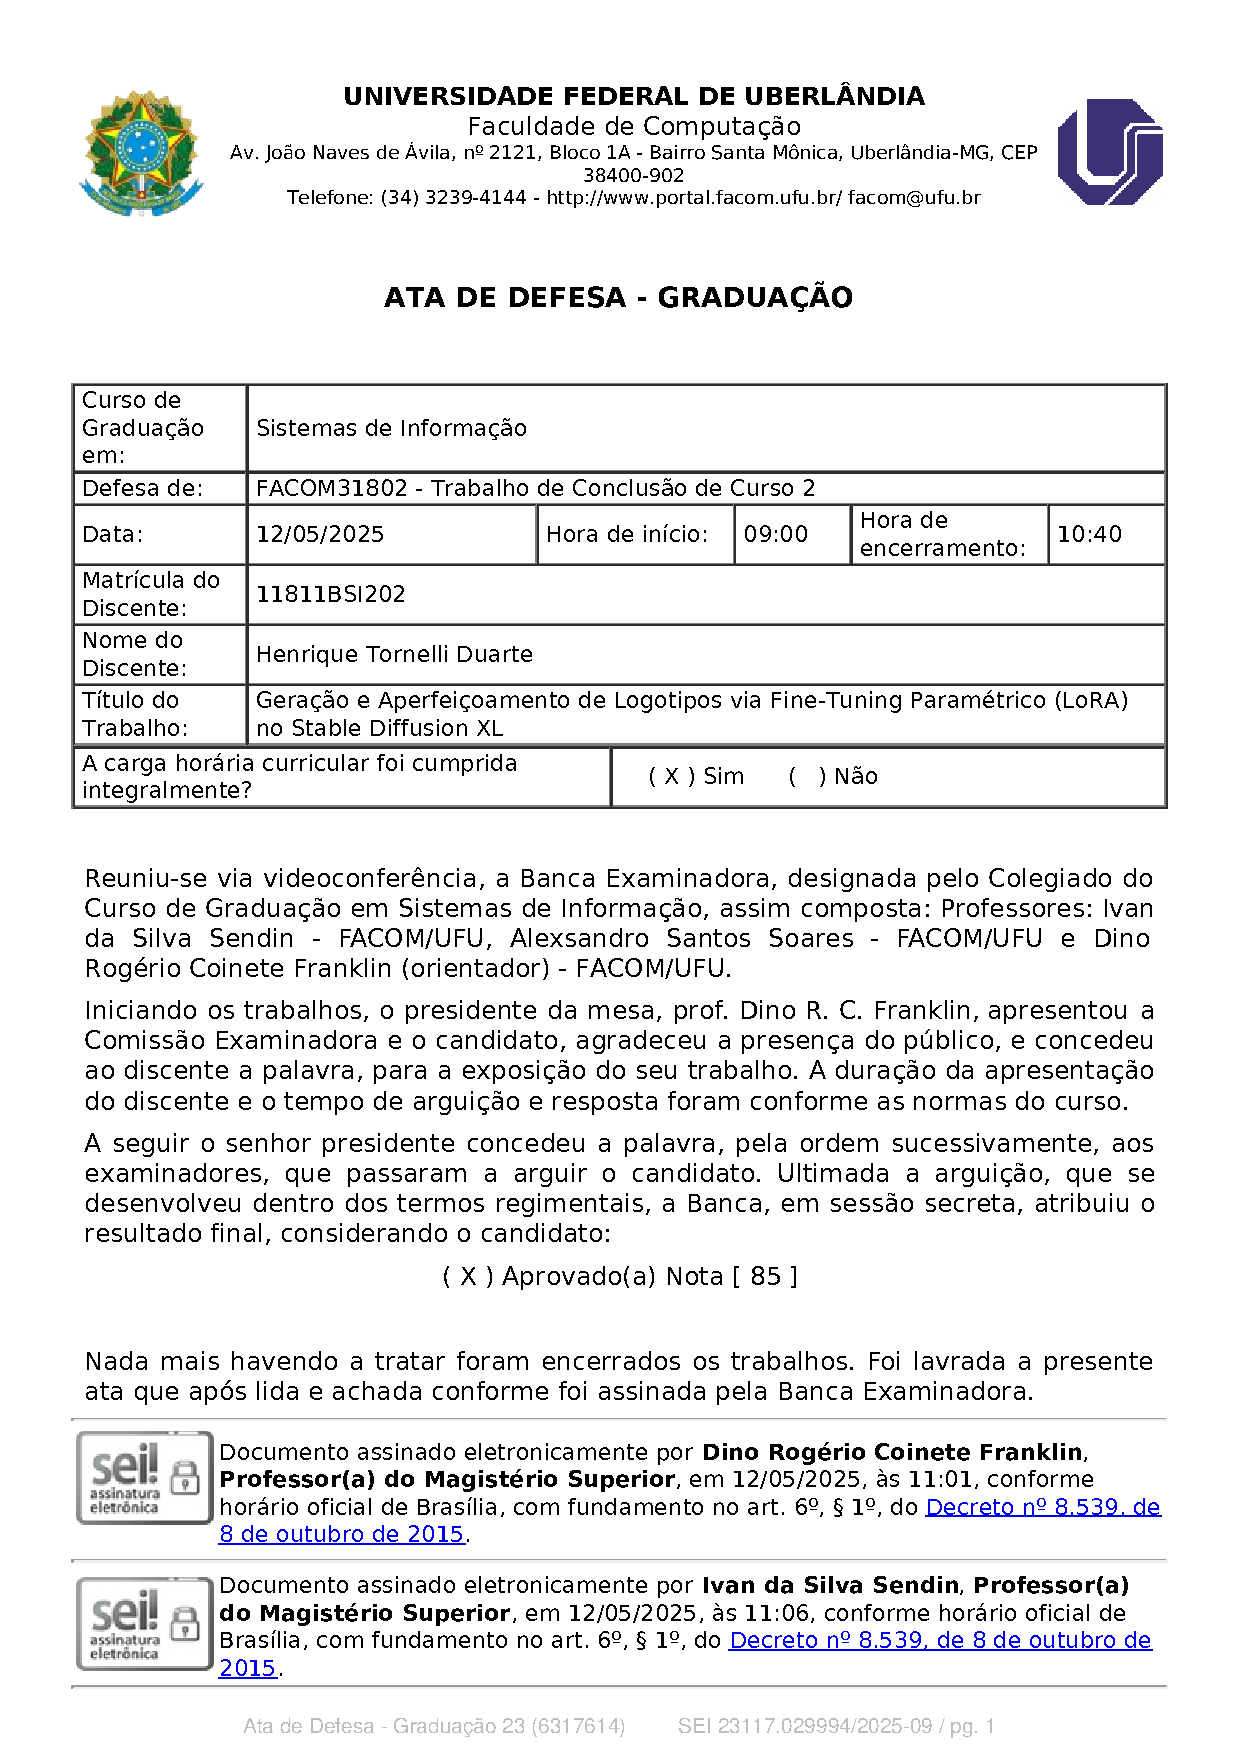
\includepdf{folhadeaprovacao_final.pdf} %TCC: depois de aprovado o trabalho, descomente esta linha e comente o próximo bloco para incluir scan da folha de aprovação.
%
\begin{folhadeaprovacao}

  \begin{center}
    {\ABNTEXchapterfont\large\imprimirautor}

    \vspace*{\fill}\vspace*{\fill}
    {\ABNTEXchapterfont\bfseries\Large\imprimirtitulo}
    \vspace*{\fill}
    
    \hspace{.45\textwidth}
    \begin{minipage}{.5\textwidth}
        \imprimirpreambulo
    \end{minipage}%
    \vspace*{\fill}
   \end{center}
    
    % Trabalho aprovado. \imprimirlocal, 24 de novembro de 2012: %TCC:

   \assinatura{\textbf{\imprimirorientador} \\ Orientador}  
   \assinatura{\textbf{Professor Alexsandro Santos Soares} \\ Convidado 1} %TCC:
   \assinatura{\textbf{Professor Ivan da Silva Sendin} \\ Convidado 2} %TCC:
      
   \begin{center}
    \vspace*{0.5cm}
    {\large\imprimirlocal}
    \par
    {\large\imprimirdata}
    \vspace*{1cm}
  \end{center}
  
\end{folhadeaprovacao}
% ---


%%As seções dedicatória, agradecimento e epígrafe não são obrigatórias.
%%Só as mantenha se achar pertinente.

% ---
% Dedicatória
% ---
\begin{dedicatoria}
   \vspace*{\fill}
   \centering
   \noindent
   \textit{Dedico à minha esposa \textbf{Karoliny} e à minha filha \textbf{Valentina}, minha força diária e razão maior de seguir em frente. Sem o amor, o apoio e a paciência de vocês, eu teria desistido no caminho.}
   \vspace*{\fill}
\end{dedicatoria}
% ---

% ---
% Agradecimentos
% ---
\begin{agradecimentos}
    Agradeço, em primeiro lugar, a minha familia \textbf{Karoliny} e \textbf{Valentina} e aos meus pais \textbf{Elizângela} e \textbf{Marcelo}, que me deram a educação e a base necessárias para enfrentar os desafios da vida.

    Sou grato aos amigos que tornaram a jornada universitária mais leve e divertida — \textbf{Gabriel}, \textbf{Guilherme}, \textbf{Vitor} e \textbf{João Vitor}. Obrigado por transformarem os momentos mais difíceis nos mais memoráveis.
    
    Ao meu amigo internacionalmente especial \textbf{Joni Innanen}, por manter viva a inspiração de buscar novos horizontes e acreditar que a formação acadêmica pode abrir portas no exterior.
    
    Registro especial apreço ao meu orientador, \textbf{Prof.\ Dino Franklin}, pela confiança, pela orientação constante e por não desistir mesmo durante meus períodos de ausência. Extendo meus agradecimentos aos professores \textbf{Alexsandro}, \textbf{Autran}, \textbf{Rivalino} e \textbf{Willian}, cujos ensinamentos marcaram profundamente minha trajetória e continuam a influenciar meu desenvolvimento.
\end{agradecimentos}
% ---


% ---
% Epígrafe
% ---
% \begin{epigrafe}
%     \vspace*{\fill}
% 	\begin{flushright}
% 		\textit{``Alguma citação que ache conveniente? \lipsum[10]''} %TCC:
% 	\end{flushright}
% \end{epigrafe}
% ---


% ---
% Resumo
% ---
%TCC:
\begin{resumo}
    Esta dissertação avalia técnicas de \emph{ajuste fino} (fine-tuning) aplicadas ao \textbf{Stable Diffusion XL} (SDXL), versão de alta resolução do modelo de difusão latente, com foco na adaptação leve oferecida pelo \textbf{LoRA}—\emph{Low-Rank Adaptation}, inserção de matrizes de baixa dimensão que exige bem menos parâmetros. Prepararam-se seis conjuntos de dados específicos (\emph{datasets}): estrutura tipográfica (\emph{wordmark}), símbolo gráfico (\emph{iconic}) e estilização (\emph{minimalistic}, \emph{vintage} e \emph{cartoon}). Cada conjunto foi treinado durante 10 épocas (\emph{epoch}: ciclo completo em que o modelo percorre todo o conjunto de treinamento), empregando taxas de aprendizado distintas para o modulador de texto (encoder CLIP-Text) e para a U-Net responsável pela imagem.

    A fase experimental gerou 8\,640 amostras, combinando sistematicamente a escala de orientação \emph{CFG} (Classifier-Free Guidance), o número de etapas de \emph{denoising} (\emph{Steps}) e algoritmo de amostragem (\emph{sampler}). As métricas adotadas incluíram similaridade CLIP (aderência semântica), acurácia OCR (legibilidade do texto) e avaliação humana. Os resultados mostram que o ajuste fino via LoRA guia a difusão para um espaço de soluções mais restrito e coerente, reduzindo ruído visual e variações indesejadas. A legibilidade textual saltou de 37\% no modelo base para 88\% após o ajuste, superando 92\% quando se aplicou o pós-processamento de correção de texto (\emph{fix-text}). A análise qualitativa confirma que a abordagem conserva o estilo desejado, melhora a precisão do nome da marca e permite diminuir o número total de etapas de amostragem. Conclui-se que o LoRA, aliado a curadoria criteriosa de dados e ajuste fino de hiperparâmetros, é a alternativa mais eficaz para especializar o SDXL na geração automática de logomarcas.  
    
    \vspace{\onelineskip}
    
    \noindent
    \textbf{Palavras-chave}: geração de imagens, Stable Diffusion XL, LoRA, logomarcas, ajuste fino.
 \end{resumo}
% ---


% ---
% inserir lista de ilustrações
% ---
\pdfbookmark[0]{\listfigurename}{lof}
\listoffigures*
\cleardoublepage
% ---


% ---
% inserir lista de tabelas
% ---
\pdfbookmark[0]{\listtablename}{lot}
\listoftables*
\cleardoublepage
% ---


% ---
% inserir lista de abreviaturas e siglas
% ---
%TCC:
\begin{siglas}
    \item[SD] Stable Diffusion
    \item[SDXL] Stable Diffusion XL
    \item[LoRA] Low-Rank Adaptation
    \item[TI] Textual Inversion
    \item[DB] DreamBooth
    \item[CFG] Classifier-Free Guidance (escala de orientação)
    \item[LR] Learning Rate (taxa de aprendizado)
    \item[OCR] Optical Character Recognition
    \item[GPU] Graphics Processing Unit
    \item[VRAM] Video Random-Access Memory
    \item[FP16] Half-precision floating point (16 bits)
    \item[SDE] Stochastic Differential Equation (formulação de difusão)
    \item[ODE] Ordinary Differential Equation (formulação determinística)
    \item[DPM] Denoising Probabilistic Model (família de salgoritmos de amostragem)
    \item[CLIP] Contrastive Language-Image Pre-training
    \item[PEFT] Parameter-Efficient Fine-Tuning
  \end{siglas}
% ---


%% ---
%% inserir lista de símbolos, se for adequado ao trabalho. %TCC:
%% ---
%\begin{simbolos}
%  \item[$ \Gamma $] Letra grega Gama
%  \item[$ \Lambda $] Lambda
%  \item[$ \zeta $] Letra grega minúscula zeta
%  \item[$ \in $] Pertence
%\end{simbolos}
%% ---


% ---
% inserir o sumario
% ---
\pdfbookmark[0]{\contentsname}{toc}
\tableofcontents*
\cleardoublepage
% ---


% ----------------------------------------------------------
% Introdução
% ----------------------------------------------------------
%TCC:
\chapter{Introdução}

A síntese de imagens por Inteligência Artificial (IA) deu um salto decisivo em 2022
com a liberação pública do \textit{Stable Diffusion} (SD) \cite{rombach2022highresolutionimagesynthesislatent}\footnote{Disponibilizado pela Stability AI em colaboração com LAION e Eleuther AI, agosto de 2022.}.
O SD é um gerador de imagens baseado em \textbf{modelos de difusão latente}:
ele parte de uma ``imagem'' composta apenas de ruído e, etapa a etapa, aprende a
remover esse ruído até formar uma figura coerente que corresponda a uma
\emph{instrução textual} escrita pelo usuário — por exemplo, \emph{``uma cidade
futurista ao pôr do sol''}.
O diferencial está no local onde essa difusão ocorre: não no espaço de pixels,
mas em um \textbf{espaço latente} comprimido, codificado por um
\emph{Autoencoder Variacional} (VAE).  Trabalhar nesse espaço reduz
drasticamente o uso de memória e o tempo de cálculo, sem sacrificar detalhes
finos na imagem final.

O pipeline é composto por três blocos principais.  
O VAE comprime imagens reais e reconstrói amostras geradas, atuando
como ponte entre pixels e vetores latentes.  
A \emph{U-Net} — rede convolucional em formato de ``U'', com camadas de
contração e expansão — executa o processo de \emph{denoising}, estimando em
cada passo quanto ruído ainda deve ser removido.  
Por fim, o texto colocado pelo usuário é convertido em vetores semânticos pelo
CLIP (\emph{Contrastive Language-Image Pre-training}), que alinha a
descrição com a imagem em construção, garantindo aderência semântica entre
palavras e pixels.

Essa combinação de arquitetura eficiente e licença aberta tornou o Stable
Diffusion relevante em múltiplos contextos: ele pode rodar em GPUs de consumo
doméstico, é facilmente customizável — inclusive via \emph{treinamento
adicional} leve — e já encontra aplicações em arte digital, design de jogos,
publicidade e prototipagem de produtos.

\subsection*{Evolução das versões do Stable Diffusion}

\begin{itemize}
  \item \textbf{SD 1.4} (ago 2022) — primeira versão pública, treinada em 512 px com CLIP ViT-L/14; popularizou o texto-para-imagem de código aberto.  
  \item \textbf{SD 1.5} (out 2022) — refinamento da 1.4, com dataset filtrado e remoção de artefatos, mantendo arquitetura U-Net original.  
  \item \textbf{SD 2.0} (nov 2022) — troca do encoder textual para OpenCLIP, treinamento de 1 → 768 px, introdução de \emph{depth-guidance} e modelo upscaler \(4\times\).  
  \item \textbf{SD 2.1} (dez 2022) — ajuste fino da 2.0 com dataset ampliado, melhor equilíbrio cromático e menor suscetibilidade a ruídos.  
  \item \textbf{SDXL (1.0)} (jul 2023) — arquitetura expandida: U-Net \(3\times\) maior, duplo encoder textual, resolução nativa 1024 px, e estágio opcional de refinamento \emph{image-to-image} para realce de detalhes. \cite{podell2023sdxlimprovinglatentdiffusion}
\end{itemize}

\begin{figure}[H]
    \centering
	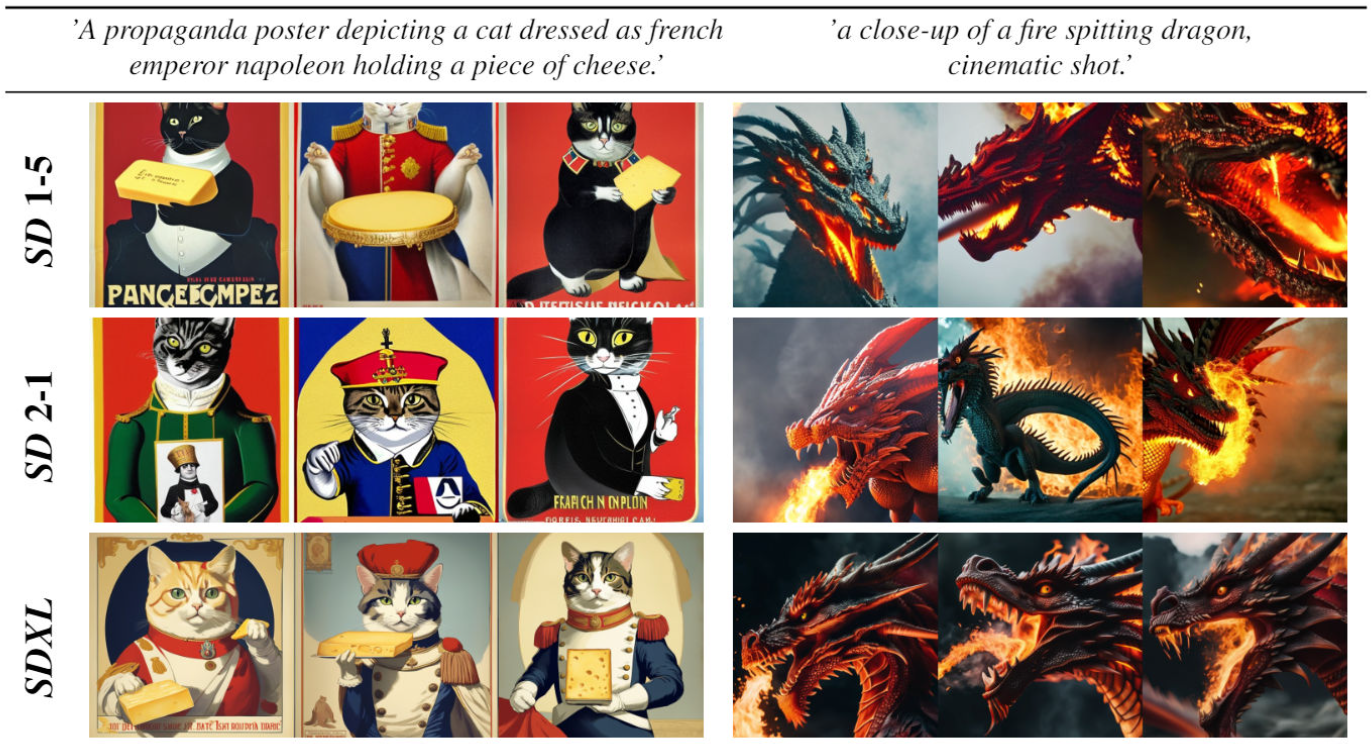
\includegraphics[width=0.85\linewidth]{figuras/comparison-sd-1.png}
	\caption[Comparação de versões do Stable Difusion]{Comparação da saída do SDXL com as versões anteriores do Stable Difusion.}
	\label{fig:comparisonSd1}
\end{figure}

Cada iteração aprimorou compreensão semântica e qualidade visual, mas manteve a filosofia de código aberto e o pipeline de difusão latente.

Esses avanços tornaram o SD e suas derivações a base de inúmeras aplicações — ilustração digital, arte conceitual, publicidade e prototipagem de produtos — democratizando a geração de conteúdo visual. Contudo, tarefas que exigem controle estilístico preciso, como a criação de logomarcas, continuam desafiadoras. Logomarcas demandam legibilidade tipográfica, composição equilibrada e consistência de estilo; o SDXL base, com instruções textuais sucintas, ainda tende a produzir composições desconexas ou texto ilegível.

\begin{figure}[H]
    \centering
	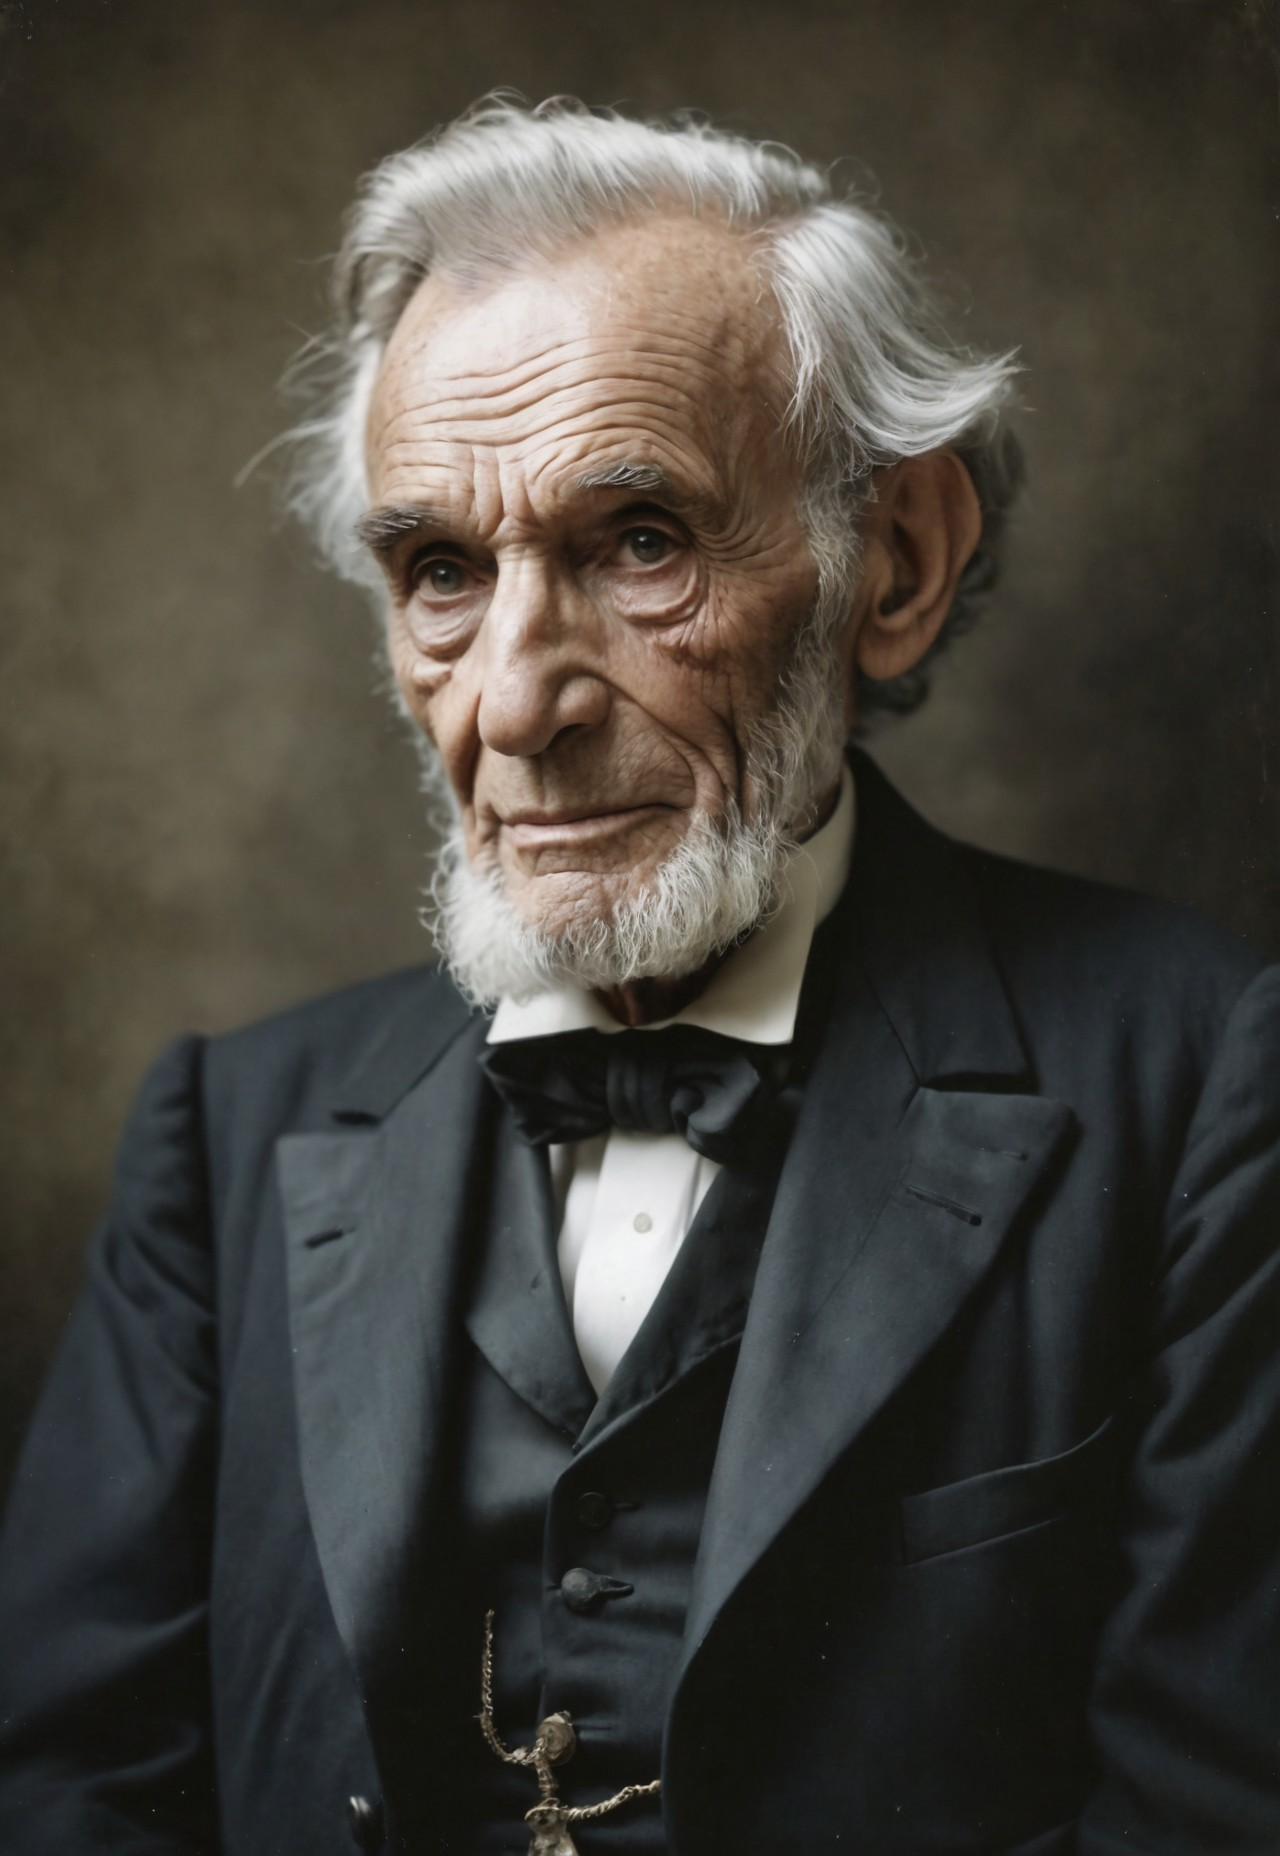
\includegraphics[width=0.35\linewidth]{figuras/sdxl-sample-1.jpeg}
	\caption[Exemplo realista de saída do SDXL]{Exemplo de saída do SDXL: Fotografia realista de um homem com vestimenta formal. Instrução textual completa pode ser encontrada \href{https://civitai.com/images/45346112}{neste endereço}.}
	\label{fig:sdxlSample1}
\end{figure}

\subsection*{Ajuste Fino}

Com estes avanços, a geração de imagens tornou-se um processo acessível: basta fornecer uma descrição em texto e, em segundos, o algoritmo transforma ruído em figuras detalhadas e realistas.

Todavia, esses modelos nascem genéricos; foram treinados em enormes coleções de imagens da internet. Quando surge a necessidade de especializar a saída — seja para um estilo artístico particular, uma estética de marca ou qualquer domínio visual específico — recorre-se a um ajuste fino (\emph{fine-tuning}). No geral, parte-se do modelo já pré-treinado e realiza-se um breve ciclo de ajuste sobre um conjunto de exemplos cuidadosamente escolhidos. O procedimento preserva o conhecimento amplo adquirido anteriormente, mas direciona a rede a reproduzir padrões, cores e composições mais alinhados ao novo objetivo.

Dessa forma, consegue-se combinar a versatilidade de um modelo geral com a precisão de um modelo feito sob medida, sem a necessidade de treinar tudo novamente do zero.

\subsection*{Inpainting e Control Net}

Outra habilidade importante dos modelos de difusão é o \emph{inpainting}, técnica que permite editar seletivamente uma região da imagem. O usuário define uma máscara — por exemplo, o espaço vazio em um rótulo — e descreve em texto o que deve aparecer ali. O modelo mantém intacto o restante do quadro e preenche apenas a área mascarada, garantindo continuidade de cor, iluminação e textura. Esse processo é valioso quando se deseja corrigir detalhes ou inserir elementos adicionais sem recriar toda a composição.

Complementar ao \emph{inpainting} está o \emph{outpainting}, que faz o movimento inverso: expande os limites de uma imagem além de suas bordas originais. A partir de pequenas porções de contexto visual, o gerador estende a cena, completando fundos, prolongando padrões ou adicionando novos objetos de forma coerente. Na prática, essa técnica é usada para criar versões panorâmicas de ilustrações ou material publicitário em formatos variados, preservando o estilo e a continuidade estética.

Para aproximar ainda mais a geração do controle humano, surgiu o \textit{Control Net}. Trata-se de uma rede adicional acoplada ao modelo de difusão que recebe informações estruturais — mapas de bordas, profundidade, poses, segmentações — e as utiliza como ``grade'' durante a síntese. Enquanto a instrução textual em texto dita o conteúdo semântico, o \textit{Control Net} fixa a geometria, garantindo que linhas mestras, contornos ou silhuetas específicas sejam respeitadas. Isso destrava aplicações que exigem alinhamento preciso, como adaptação de layouts ou reinterpretação estilística de desenhos técnicos.

Quando combinadas, essas ferramentas oferecem um leque robusto de edição: o texto direciona o tema, o \textit{Control Net} define a estrutura e o \emph{inpainting}/\emph{outpainting} ajusta ou estende áreas localizadas. O resultado é um fluxo de trabalho flexível, no qual o usuário pode tanto criar imagens do zero quanto aprimorar e adaptar ilustrações existentes, mantendo controle sobre forma, escala e consistência visual.

\begin{figure}[H]
    \centering
    \begin{subfigure}{.46\textwidth}
      \centering
      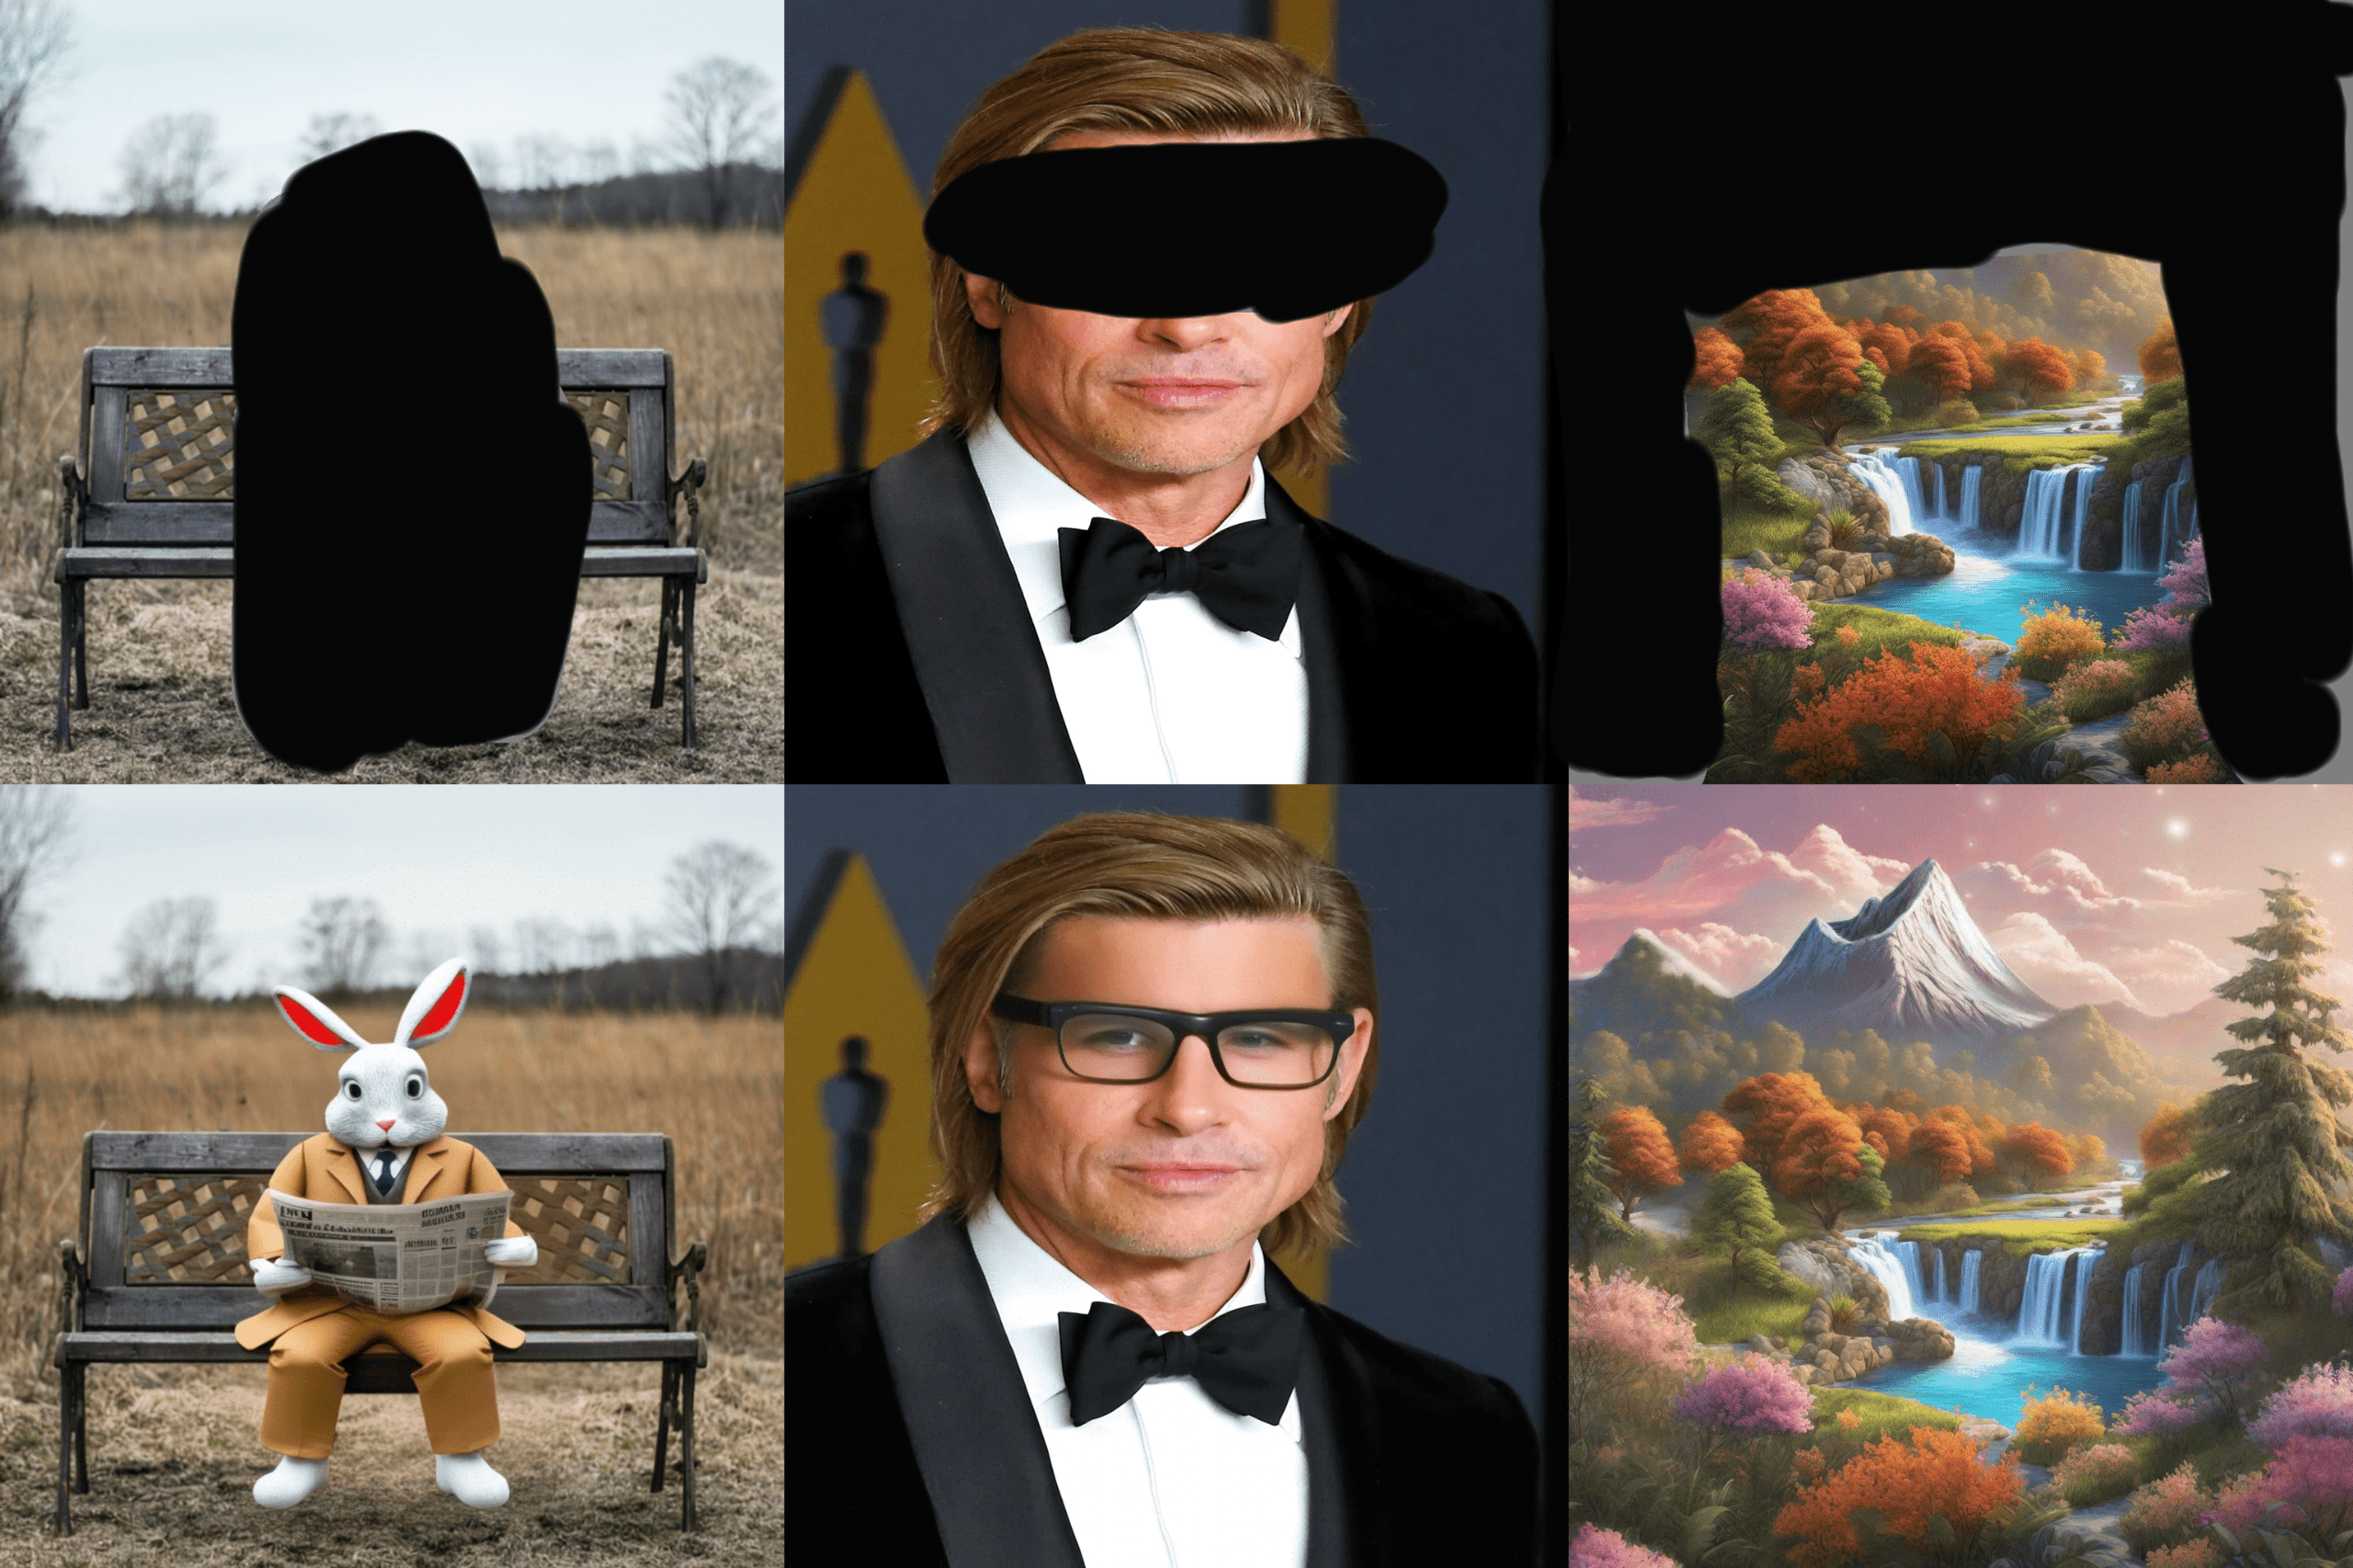
\includegraphics[width=\linewidth]{inpaint-sample-1.png}
      \caption{\emph{Inpainting} aplicado a três diferentes imagens usando máscara.}
      \label{fig:InpaintingOutpaintingControlNetSub1}
    \end{subfigure}
    \begin{subfigure}{.417\textwidth}
      \centering
      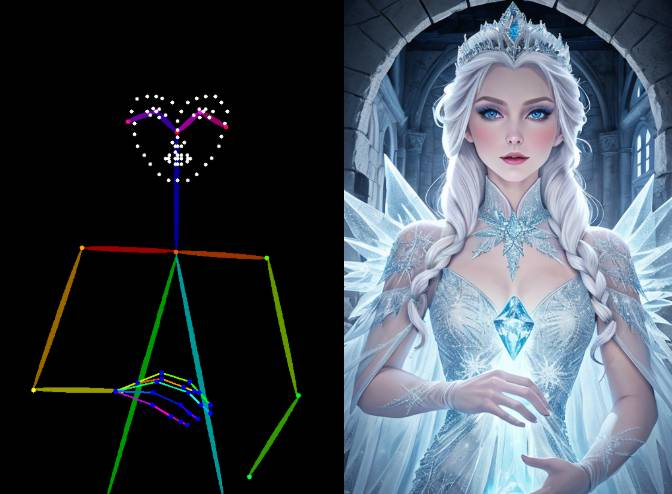
\includegraphics[width=\linewidth]{controlnet-sample-1.jpg}
      \caption{\textit{ControlNet} baseado em uma pose gerando uma imagem.}
      \label{fig:InpaintingOutpaintingControlNetSub2}
    \end{subfigure}
    \caption{Demonstração do conceito de \emph{inpainting}/\emph{outpainting} e \textit{Control Net}.}
    \label{fig:InpaintingOutpaintingControlNet}
\end{figure}

\section{Problema}

Apesar dos avanços trazidos pelo SDXL, a geração automática de logomarcas ainda enfrenta limitações que comprometem sua adoção prática. Quando se utilizam instruções textuais curtas — por exemplo, apenas o nome da marca seguido de um adjetivo de estilo — o modelo raramente entrega uma identidade visual consistente: surgem composições incoerentes, símbolos desconexos ou mesmo imagens abstratas sem qualquer hierarquia gráfica típica de um logotipo.

Para tentar contornar essas falhas, muitos usuários recorrem à engenharia de \emph{prompt}: descrições longas, repletas de qualificadores (família tipográfica, paleta de cores, alinhamento, espessura de traço, proporção do ícone), que buscam direcionar o modelo em cada detalhe. Embora possa haver melhoria pontual, esse processo é complexo, instável, demanda experiência e contraria a premissa de agilidade que tornou os modelos de difusão tão atraentes.

A tipografia é outro ponto crítico. Mesmo instruções textuais detalhadas não impedem o SDXL base de gerar letras distorcidas, glifos inexistentes ou duplicações aleatórias. Em muitos casos, o texto some por completo ou se mistura ao fundo, tornando a logomarca inutilizável.

\begin{figure}[H]
    \centering
	
\includegraphics[width=\linewidth]{figuras/problem-1.png}
	\caption{Demonstração de saídas com instruções textuais relacionadas a logomarcas.}
	\label{fig:problem1}
\end{figure}

\begin{figure}[H]
    \centering
	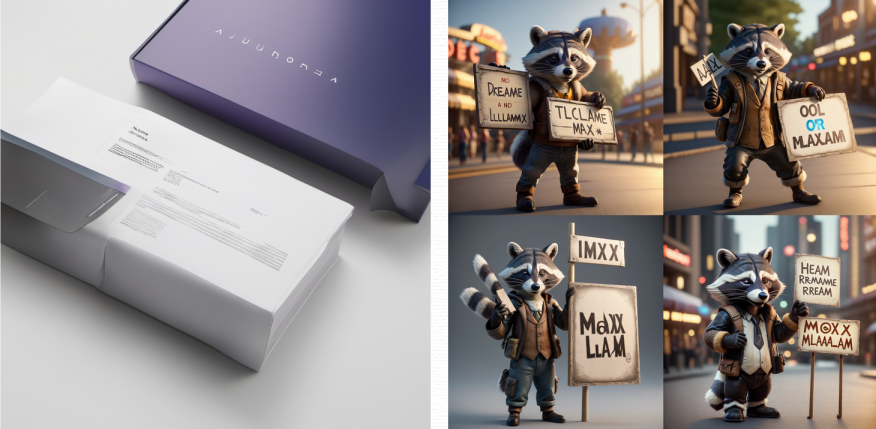
\includegraphics[width=0.8\linewidth]{figuras/problem-3.png}
	\caption{Demonstração de saídas com instruções textuais relacionadas a texto.}
	\label{fig:problem2}
\end{figure}

\subsection*{Ilustração Prática do Problema}

Para ilustrar de forma objetiva as dificuldades enfrentadas pelo SDXL sem qualquer adaptação, foram geradas amostras para três variações de instrução textual, todos visando produzir uma logomarca minimalista para a marca fictícia ``AURORA'':

\begin{enumerate}
    \item \texttt{text AURORA, ultra-thin spacing, luxurious minimal look}
    \item \texttt{logo, text AURORA, ultra-thin spacing, luxurious minimal look}
    \item \texttt{logo, wordmark, text ``AURORA'', ultra-thin spacing, luxurious minimal look}
\end{enumerate}

As figuras a seguir apresentam, em ordem, quatro amostras produzidas para cada instrução textual (semente fixa e conjuntos de 4 imagens).

\begin{figure}[H]
    \centering
	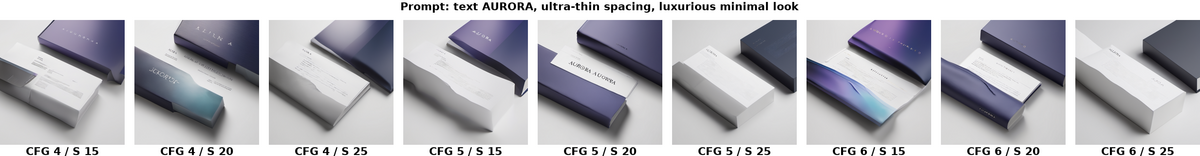
\includegraphics[width=\linewidth]{figuras/resultados/good/base/p1_batch0.png}
    \caption{Instrução textual 1 da ilustração do problema: text AURORA, ultra-thin spacing, luxurious minimal look}
    \label{fig:sdxl_base_p1}
\end{figure}

\begin{figure}[H]
    \centering
	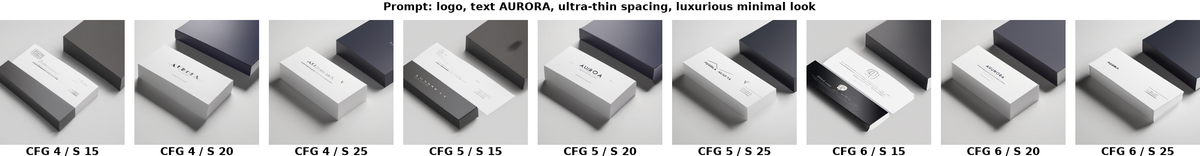
\includegraphics[width=\linewidth]{figuras/resultados/good/base/p2_batch0.png}
    \caption{Instrução textual 2 da ilustração do problema: logo, text AURORA, ultra-thin spacing, luxurious minimal look}
    \label{fig:sdxl_base_p2}
\end{figure}

\begin{figure}[H]
    \centering
	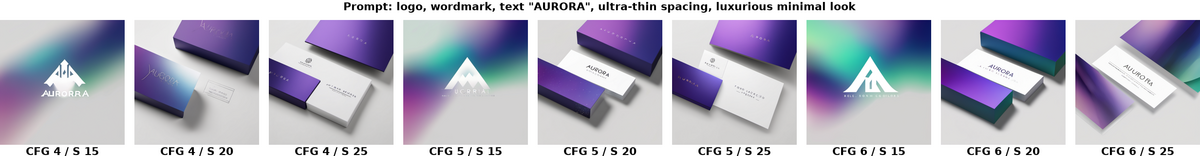
\includegraphics[width=\linewidth]{figuras/resultados/good/base/p3_batch0.png}
    \caption{Instrução textual 3 da ilustração do problema: logo, wordmark, text ``AURORA'', ultra-thin spacing, luxurious minimal look}
    \label{fig:sdxl_base_p3}
\end{figure}

Mesmo quando o termo logo ou \emph{wordmark} é explicitado, o modelo raramente entrega um resultado que possa ser reconhecido como logomarca. Observam-se principalmente:

\begin{itemize}
    \item Objetos ou emblemas abstratos que não contêm texto algum;
    \item Agrupamentos de letras ilegíveis ou com glifos inexistentes;
    \item Falta de hierarquia visual, com símbolos dispersos e ausência de área de respiro;
    \item Variação imprevisível de cores e texturas, contrariando a estética ``luxurious minimal'';
    \item Embora a terceira instrução textual apresente um layout que remete a uma logomarca, o texto resultante ainda é inválido ou completamente ausente.
\end{itemize}

A comparação direta entre as três tentativas deixa claro que simplesmente adicionar mais palavras-chave a instrução textual não resolve o problema: o SDXL continua sem diretriz sólida sobre como estruturar texto e símbolo como elementos de identidade visual.

\section{Hipótese}

A hipótese central deste trabalho é que a aplicação estruturada e específica de técnicas de ajuste fino pode melhorar significativamente a qualidade geral das logomarcas geradas por modelos como o SDXL, independentemente da complexidade das instruções textuais fornecidas.

Mais especificamente, acredita-se que o uso dessa técnica de ajuste fino poderá:

\begin{itemize}
    \item Melhorar a consistência visual geral das imagens geradas, tornando-as mais próximas da estrutura e composição típicas de logomarcas;
    \item Reduzir significativamente a necessidade de instruções textuais detalhadas e complexas por parte do usuário;
    \item Facilitar o processo criativo, oferecendo resultados úteis e visualmente coerentes com menos tentativas;
    \item Contribuir para melhorias gerais na legibilidade e coerência dos textos, embora reconhecendo que esta é uma consequência secundária e não uma garantia absoluta;
    \item Oferecer uma abordagem documentada e replicável (\ref{repo}), contribuindo diretamente para a comunidade científica e criativa.
\end{itemize}

\section{Objetivo}

O objetivo geral deste trabalho é propor, implementar e validar uma abordagem prática e acessível para geração automática de logomarcas, melhorando a qualidade geral das imagens geradas por modelos generativos como o SDXL, independentemente do nível de detalhe da instrução textual fornecido.

Para atingir esse objetivo geral, foram definidos objetivos específicos claros:

\begin{itemize}
    \item Criar conjuntos de dados estruturados e diversificados adequados ao treinamento especializado dos modelos;
    \item Realizar ajustes finos com estratégias específicas para direcionar melhor o foco visual e a coerência das logomarcas geradas;
    \item Construir fluxos simples e intuitivos que facilitem a geração consistente de logomarcas sem exigir conhecimentos avançados de criação de instruções textuais;
    \item Documentar detalhadamente todos os procedimentos, hiperparâmetros e scripts utilizados (\ref{repo}), facilitando a replicação do processo por outros pesquisadores e profissionais criativos;
    \item Avaliar objetivamente a melhoria obtida nos resultados gerados por meio de métricas quantitativas e qualitativas.
\end{itemize}

\section{Resultados Esperados}

Ao concluir este estudo, espera-se demonstrar os seguintes resultados e contribuições:

\begin{itemize}
    \item Uma melhora geral significativa na qualidade visual e na consistência das logomarcas geradas, independentemente do nível de detalhamento das instruções textuais;
    \item Uma redução notável da complexidade exigida nas instruções textuais, tornando a criação automática mais acessível;
    \item Uma documentação completa e replicável (\ref{repo}), permitindo a reprodução do processo por outros pesquisadores e profissionais.
\end{itemize}

Em resumo, este trabalho busca auxiliar a comunidade científica e profissional a explorar melhor o potencial dos modelos generativos modernos, propondo uma abordagem prática, acessível e documentada para tornar a criação automática de logomarcas uma tarefa mais eficaz e produtiva.

% ---


% ----------------------------------------------------------
% Revisão Bibliográfica
% ----------------------------------------------------------
%TCC:
\chapter{Revisão Bibliográfica}

\section{Stable Diffusion: Fundamentos e Arquitetura}

O Stable Diffusion é um modelo generativo de imagens baseado em difusão latente, introduzido por Rombach em 2022 \cite{rombach2022highresolutionimagesynthesislatent}. Ele representa um avanço significativo na geração de imagens de alta qualidade, combinando eficiência computacional com flexibilidade na geração condicionada por texto.

\subsection{Difusão Latente}

Diferentemente dos modelos de difusão tradicionais que operam diretamente no espaço de pixels, o Stable Diffusion realiza o processo de difusão em um espaço latente comprimido. Isso é possível graças ao uso de um \textit{autoencoder} variacional (VAE), que codifica imagens de alta dimensão em representações latentes de menor dimensão. Essa abordagem reduz significativamente o custo computacional e permite a geração de imagens de alta resolução com recursos computacionais mais acessíveis.

\subsection{Arquitetura do Modelo}

\begin{enumerate}
    \item \textbf{Codificador de Texto (CLIP)}: Utiliza o modelo CLIP para transformar instruções textuais textuais em \textit{embeddings} semânticos que condicionam a geração de imagens.
    \item \textbf{Rede U-Net Condicionada}: Uma rede neural convolucional que realiza o processo de \textit{denoising} no espaço latente, guiada pelos \textit{embeddings} textuais.
    \item \textbf{Decodificador VAE}: Reconstrói a imagem final a partir da representação latente \textit{denoised}, retornando ao espaço de pixels.
\end{enumerate}

\begin{figure}[H]
    \centering
	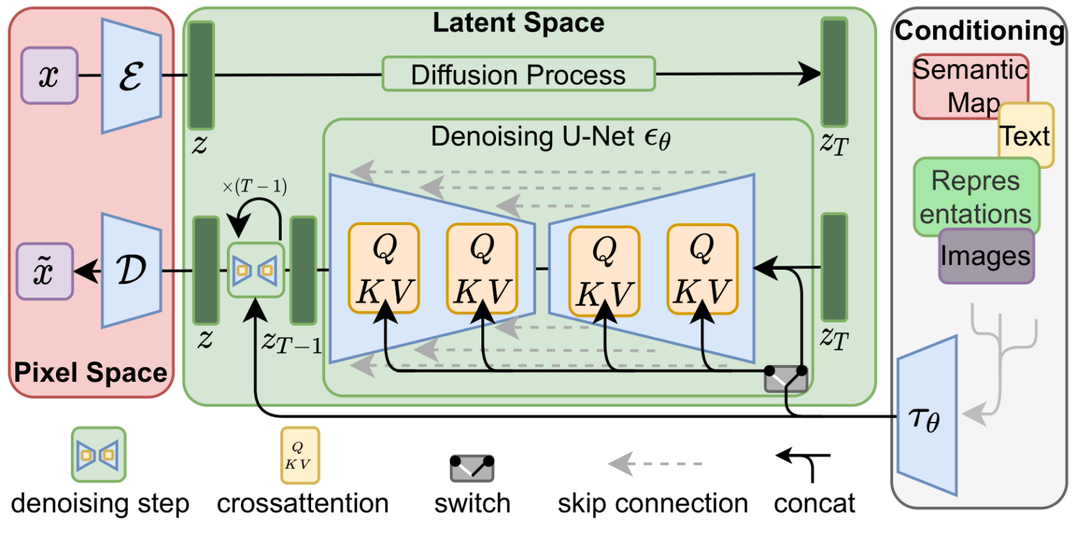
\includegraphics[width=0.9\linewidth]{sdxl-flow.png}
	\caption[Diagrama do fluxo lógico dos modelos de difusão latente]{Representação das etapas de geração no Stable Diffusion, desde a semente e ruído inicial até a geração da imagem via decodificador VAE.}
	\label{fig:diagramaFluxoStableDiffusion}
\end{figure}

\subsection{Processo de Geração}

O processo começa pela transformação da instrução textual em vetores numéricos, chamados de \emph{embeddings} semânticos, por meio do modelo CLIP (do inglês \emph{Contrastive Language-Image Pre-training}, ``pré-treinamento contrastivo de texto e imagem''). O CLIP, treinado em milhões de pares imagem-texto, projeta frases e figuras no mesmo espaço vetorial, de modo que conteúdos semelhantes fiquem próximos. Paralelamente, um Autoencoder Variacional (VAE, do inglês \emph{Variational Autoencoder}) codifica o que será a ``imagem-alvo'' — inicialmente puro ruído no modo \emph{text-to-image} — em uma representação comprimida no espaço latente.

Três parâmetros controlam a dinâmica dessa geração: a \textbf{seed} (semente aleatória que determina o ruído inicial e garante reprodutibilidade), o número de \textbf{steps} (iterações de remoção de ruído) e a escala \textbf{CFG} (\emph{Classifier-Free Guidance}), que define quão fortemente o modelo deve seguir a descrição textual em vez de sua distribuição interna de imagens.

A etapa central é a difusão reversa (\emph{denoising}), conduzida por uma rede neural em formato de ``U'' — a \emph{U-Net}. A geração inicia com o ruído latente; a cada iteração, a U-Net recebe o latente atual e os embeddings do texto e estima o ruído residual que precisa ser removido. O \emph{scheduler} (agenda de ruído) define o cronograma exato de remoção, especificando a fração de perturbação a retirar em cada passo. Em seguida, o \emph{sampler} (algoritmo de amostragem, como DDIM ou Euler) aplica as fórmulas que atualizam o latente de forma estável, obedecendo às instruções do scheduler. Esse ciclo se repete pelos \emph{steps} configurados, até que o ruído se aproxime de zero e a estrutura latente reflita um esboço coerente da imagem desejada.

Por fim, a representação latente refinada é decodificada de volta ao espaço de pixels pelo VAE, gerando a imagem final. O decodificador atua como um filtro de alta resolução, convertendo a compressão latente em detalhes visuais ricos, respeitando as cores, texturas e formas indicadas pela instrução textual.

\begin{figure}[H]
    \centering
	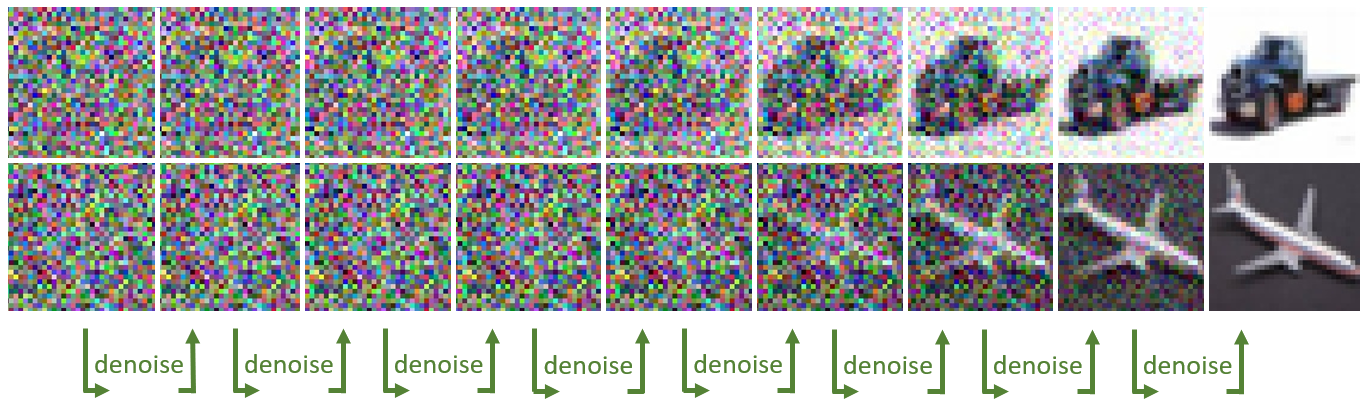
\includegraphics[width=\linewidth]{denoising.png}
	\caption{Ilustração do processo de difusão reversa.}
	\label{fig:denoising}
\end{figure}

\subsection{Stable Diffusion XL (SDXL): Avanços na Geração de Imagens de Alta Resolução}

\begin{figure}[H]
    \centering
        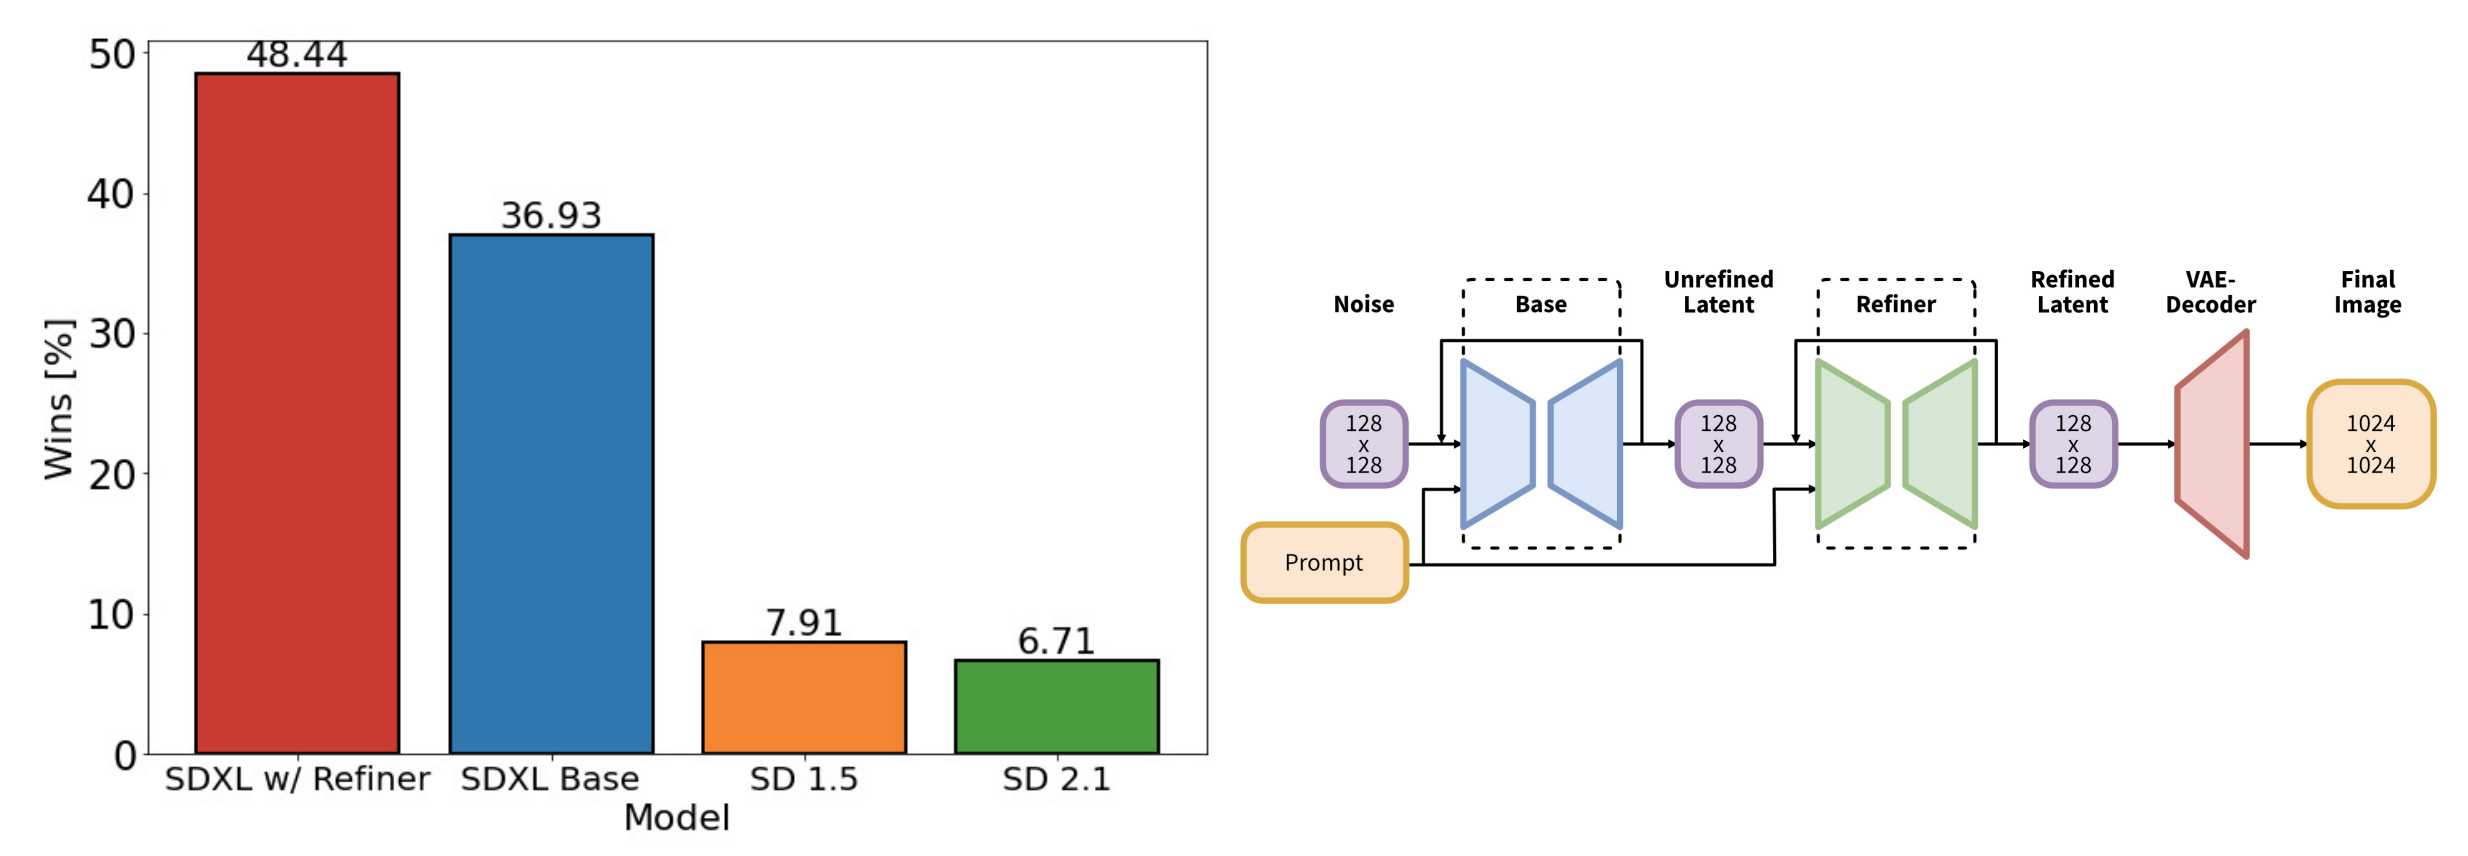
\includegraphics[width=1.0\linewidth]{comparacao_pipeline_sdxl.png}
        \caption[Comparação e pipeline em duas etapas do SDXL]{À esquerda, comparação da preferência dos usuários entre SDXL e versões anteriores do Stable Diffusion. À direita, diagrama do pipeline em duas etapas, com geração inicial e refinamento em alta resolução usando a mesmo instrução textual e autoencoder.}
        \label{fig:comparacaoPipelineSdxl}
\end{figure}

O Stable Diffusion XL (SDXL) representa uma evolução significativa em relação ao modelo original de difusão latente. Introduzido por Podell em 2023 \cite{podell2023sdxlimprovinglatentdiffusion}, o SDXL aprimora a qualidade e a fidelidade das imagens geradas, especialmente em resoluções mais altas, mantendo a eficiência computacional.

\begin{figure}[H]
    \centering
        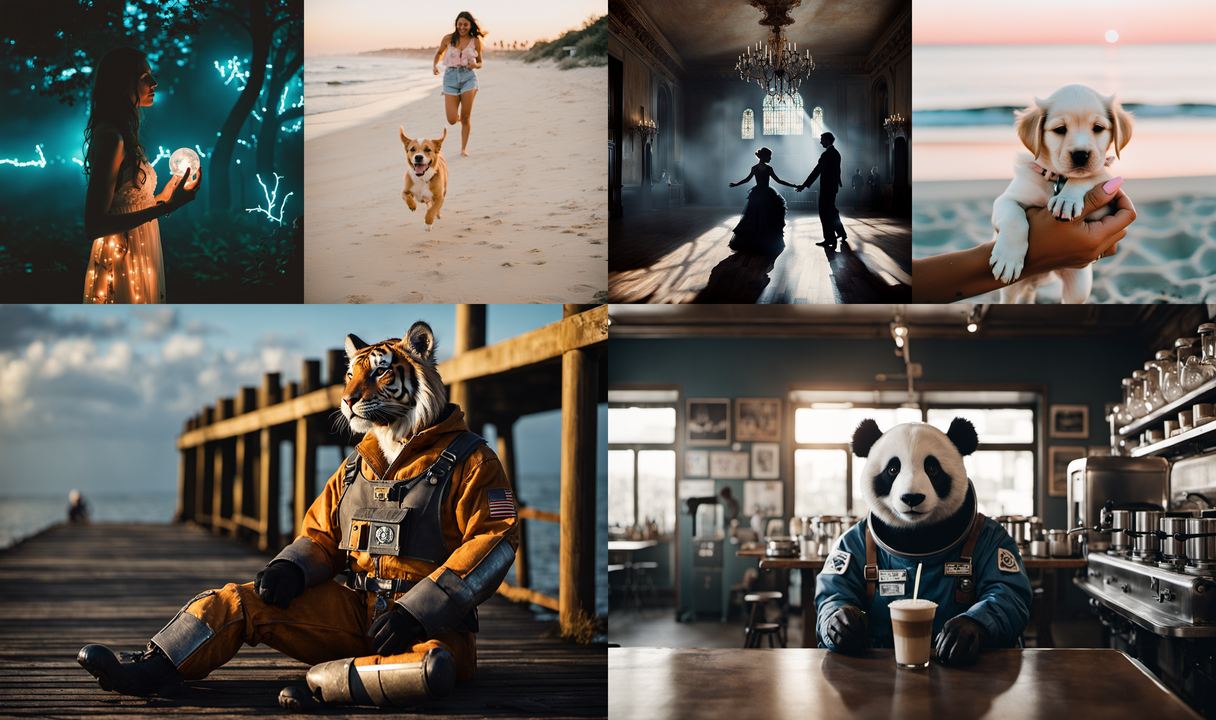
\includegraphics[width=\linewidth]{sdxl-sample-2.png}
        \caption{Imagens geradas usando SDXL.}
        \label{fig:sdxlSample2}
\end{figure}

\subsubsection*{Principais Melhorias Arquiteturais}

\begin{itemize}
    \item \textbf{U-Net ampliada}: A rede U-Net do SDXL foi aumentada em profundidade e largura — mais camadas convolucionais, mais blocos residuais e seções de auto-atenção — chegando a cerca de três vezes o número de parâmetros do modelo original. Esse reforço de capacidade permite capturar texturas mais finas e relações espaciais de longo alcance, produzindo imagens com detalhes nítidos e composição mais coerente.
    \item \textbf{Duplo Codificador de Texto}: O SDXL incorpora um segundo codificador de texto, ampliando o contexto de atenção cruzada. Isso resulta em uma compreensão semântica mais profunda das instruções textuais, melhorando a coerência entre texto e imagem.
    \item \textbf{Treinamento em Múltiplas Proporções}: Diferentemente do SD, que era treinado principalmente em imagens quadradas, o SDXL foi treinado em múltiplas proporções de aspecto, aumentando sua versatilidade na geração de imagens em diferentes formatos.
    \item \textbf{Modelo de Refinamento}: O SDXL introduz um modelo de refinamento que aplica uma técnica de imagem para imagem pós-processamento, melhorando ainda mais a fidelidade visual das amostras geradas.
\end{itemize}

\subsection{Ajuste Fino}

Quando se deseja especializar um modelo de difusão já pré-treinado, realiza-se um ajuste fino (\emph{fine-tuning}): um curto ciclo de ajuste que utiliza exemplos específicos do domínio de interesse. Na forma clássica, esse ajuste implica desbloquear milhões de pesos, definir taxas de aprendizado precisas, monitorar métricas de validação e cuidar para não cair em sobreajuste (\textit{overfitting})\footnote{O modelo memoriza demais o conjunto de treino e perde capacidade de generalizar.}. Além do tempo de GPU, há o custo de armazenar gradientes e estados do otimizador, que cresce rapidamente em redes volumosas como as variantes do Stable Diffusion XL.

\begin{figure}[H]
    \centering
    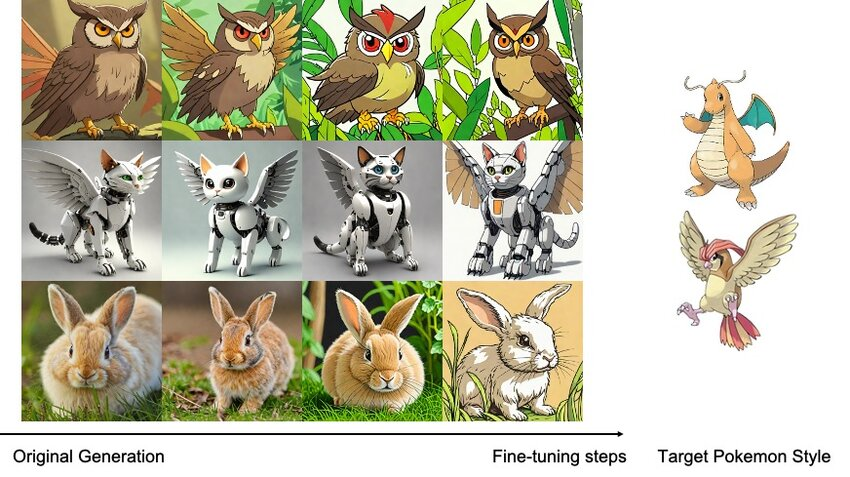
\includegraphics[width=0.9\linewidth]{finetuning-1.png}
    \caption{Ilustração demonstrando o processo de ajuste fino. Neste treinamento o foco se baseia em transformar as saídas em imagens com estilo \textit{Pokemon}.}
    \label{fig:finetuning1}
\end{figure}

Para reduzir esse impacto surgiram estratégias de adaptação eficiente, conhecidas como \textit{parameter-efficient fine-tuning}. A mais simples é a \textbf{Textual Inversion} \cite{gal2022imageworthwordpersonalizing}: treina-se um único embedding — um ``token inventado'' — que passa a representar o conceito desejado. O método é barato (poucos minutos de GPU) e não toca nos pesos do modelo, mas costuma falhar em preservar estrutura quando o conceito é visualmente complexo.

Já o \textbf{DreamBooth} introduzido por Ruiz \cite{ruiz2023dreamboothfinetuningtexttoimage}, utiliza um \emph{token} raro para ``ancorar'' o conceito e faz ajuste direcionado em todas as camadas relacionadas. O resultado é fiel ao conjunto de imagens de referência, porém o processo requer horas de processamento e muita memória, além de aumentar o risco de sobreajuste.

Entre as abordagens mais equilibradas está o \textbf{LoRA — Low-Rank Adaptation} \cite{hu2021loralowrankadaptationlarge}. A técnica insere pequenas matrizes de baixa dimensão em pontos específicos da rede; somente esses novos parâmetros são atualizados, enquanto o \emph{backbone} original permanece congelado. O LoRA combina a vantagem de arquivos leves — poucos megabytes — com a possibilidade de empilhar múltiplas adaptações diferentes, cada qual correspondendo a um estilo ou domínio. Dessa forma, consegue-se uma especialização de alta qualidade com fração do custo computacional de um fine-tuning total, preservando a flexibilidade de voltar facilmente ao comportamento original do modelo ou combinar várias adaptações conforme a necessidade.

\begin{figure}[H]
    \centering
    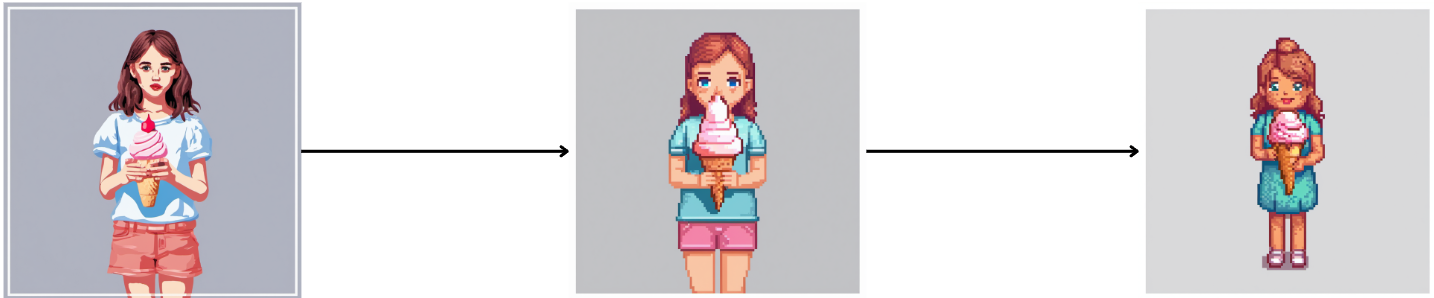
\includegraphics[width=\linewidth]{finetuning-2.png}
    \caption{Demonstração de saídas utilizando diferentes escalas de um LoRA que visa aplicar um estilo chamado de \textit{pixel-art}. A imagem à esquerda possui escala 0 (zero), a imagem central possui escala 0.5 e a imagem à direita possui escala 1.0.}
    \label{fig:finetuning2}
\end{figure}

A seguir alguns dados levantados pela comunidade em relação ao custo computacional para realizar os diferentes tipos de ajuste fino:
\begin{itemize}
      \item \textbf{Textual Inversion} Necessita \(\ge\!6\) GB de VRAM (8 GB é confortável) para resolução \(512^2\) px. Um ciclo comum usa \(\sim\!8\,000\) passos \citeonline{turn20view0}, o que leva cerca de 30-60 min numa RTX 3060 (\(\text{fp16}\), batch 1). O embedding gerado ocupa da ordem de 100-200 kB, portanto quase não impacta armazenamento.
      \item \textbf{DreamBooth} Treino completo do \textit{UNet} cabe em 16 GB de VRAM com \textit{gradient checkpointing} + \textit{bits-and-bytes} \citeonline{turn4view0}; caso o \textit{text encoder} também seja ajustado, exige pelo menos 24 GB \citeonline{turn16view0}. Experimentos usuais (400-800 passos) levam algo entre 15 min e 2 h dependendo da GPU. O checkpoint resultante adiciona 2-4 GB ao modelo base.
      \item \textbf{LoRA} O script oficial opera em 11 GB de VRAM sem truques \citeonline{turn18view0} (há relatos de 8-10 GB com \textit{xformers}). Um exemplo de 15 k passos levou \(\approx5\) h numa 2080 Ti (11 GB) \citeonline{turn21view0}. O adaptador final pesa apenas 3-20 MB, mantendo o SD/SDXL intacto e facilitando compartilhamento \citeonline{turn18view0}.
\end{itemize}

No geral podemos resumir da seguinte forma:
\begin{table}[H]
    \centering
    \small
    \setlength{\tabcolsep}{4pt}
    \begin{tabularx}{\linewidth}{|l|X|X|X|}
    \hline
    \textbf{Técnica} & \textbf{Ideia-chave} & \textbf{Vantagens} & \textbf{Limitações} \\ \hline
    Textual Inversion & Aprende um embedding textual a partir de poucas imagens & Simples; não altera os pesos do modelo & Baixa fidelidade estrutural; limitado para conceitos complexos \\ \hline
    DreamBooth & Ajuste fino em torno de um \textit{token} raro & Alta fidelidade visual & Alto custo de treino; risco de \textit{overfitting} \\ \hline
    LoRA & Injeta matrizes de baixa dimensão em camadas congeladas & Leve; modular; empilhável & Sensível à configuração de rank e \(\alpha\); efeitos variam por camada \\ \hline
    \end{tabularx}
    \caption{Técnicas de ajuste fino.}
    \label{tab:tecnicas_personalizacao}
\end{table}

\subsection{Condicionamento Estrutural e Pós-processamento de Texto}

O \textbf{ControlNet} é uma extensão modular para modelos de difusão que adiciona um canal de condicionamento explícito. Em vez de confiar apenas no vetor semântico obtido do texto, o ControlNet recebe mapas estruturais — contornos (\emph{edge maps}), profundidade (\emph{depth maps}), pose humana, segmentação semântica ou qualquer máscara binária — e os injeta como \emph{skip-connections} adicionais na U-Net. Dessa forma, o gerador respeita a geometria ou o layout fornecido, ao mesmo tempo em que mantém a criatividade nas regiões não condicionadas. O treinamento do ControlNet consiste em duplicar as camadas convolucionais da rede base e treiná-las para reconstruir o alvo enquanto o \emph{backbone} permanece congelado, o que garante compatibilidade com qualquer \emph{checkpoint} do Stable Diffusion.

\textbf{Inpainting} (preenchimento interno) é a técnica de editar apenas uma região de uma imagem existente. O usuário fornece uma máscara que define a área a ser substituída; o restante da cena serve de contexto para que o modelo gere transições suaves de cor, iluminação e textura. Já o \textbf{outpainting} (preenchimento externo) estende as bordas de uma imagem para além de seu enquadramento original. O modelo parte da borda conhecida e ``imagina'' como continuar o cenário, mantendo coerência estilística. Ambas as operações utilizam o mesmo princípio de denoising do Stable Diffusion, mas recebem máscaras diferentes no canal de ruído: no inpainting, zero na região preservada e ruído completo na região a recriar; no outpainting, o inverso — ruído fora e pixels originais dentro.

Para avaliar ou corrigir texto em imagens geradas, empregamos \textbf{EasyOCR}, biblioteca de \emph{Reconhecimento Óptico de Caracteres} (OCR, do inglês \emph{Optical Character Recognition}). O OCR converte pixels em cadeias de caracteres, permitindo verificar se o texto sintetizado coincide com o desejado. Além de servir como etapa de pós-processamento, a acurácia do OCR é aproveitada como métrica quantitativa para medir legibilidade ao longo dos experimentos.

\section{Ferramentas de Apoio}

\textbf{Kohya\_ss} \cite{kohya_ss} é uma suíte de código aberto amplamente adotada para ajuste fino em modelos da família Stable Diffusion. Disponível tanto por linha de comando quanto por interface gráfica (GUI) construída em Gradio, ela cobre todo o ciclo de fine-tuning: cria arquivos de configuração em YAML, dispara os treinos, monitora em tempo real e faz pós-processamento dos resultados. Entre os recursos práticos destacam-se o suporte a \emph{mixed-precision} e quantização — reduzindo o consumo de VRAM em GPUs modestas —, a geração automática de gráficos de perda e acurácia, e utilitários que ajudam a balancear \emph{datasets} para minimizar sobreajuste. Dessa forma, pesquisadores podem ajustar hiperparâmetros de forma iterativa e observar imediatamente o impacto sem sair da mesma ferramenta.

\textbf{ComfyUI} \cite{comfyui}, por sua vez, é um ambiente nodal para construção de fluxos de geração e edição de imagens. A interface baseia-se em um grafo visual: cada \emph{nó} representa uma operação (gerar ruído, aplicar inpainting, adicionar ControlNet, fazer upscale, calcular métrica) e possui \emph{sockets} tipados para entrada e saída, como imagem, \emph{latente}, condicionamento ou modelo. O usuário arrasta e conecta nós, definindo a ordem e o tipo de processamento de forma intuitiva; o grafo inteiro pode ser exportado em JSON, permitindo versionamento e compartilhamento entre equipes. Além da interface visual, o ComfyUI expõe uma API REST que executa o mesmo fluxo programaticamente, possibilitando automação de lotes, integração com sistemas web e coleta de metadados. Entre os controles avançados estão ajuste de semente, repetição de conjuntos de imagem e cache inteligente de nós já processados, garantindo reprodutibilidade e economia de tempo em experimentos sucessivos.

\begin{figure}[H]
    \centering
    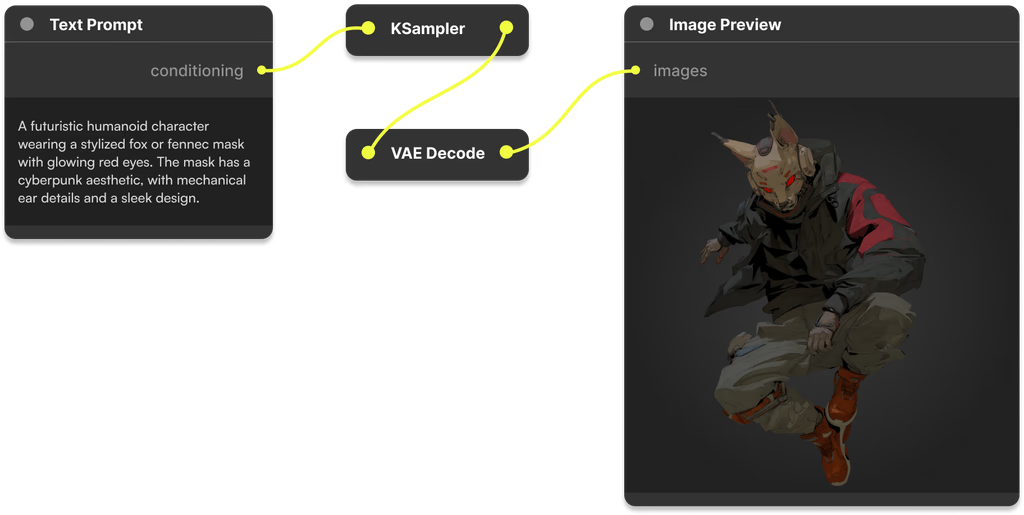
\includegraphics[width=\linewidth]{comfyui.png}
    \caption{Ilustração geral de um fluxo construído utilizando ComfyUI.}
    \label{fig:comfyUI1}
\end{figure}

\section{Estado da Arte}

A literatura recente sobre modelos de difusão mostra um campo em rápida expansão. Diversos grupos empregam esses modelos para síntese de dados, restauração de imagens e criação de conteúdo multimodal. Trabalhos como o de McWilliams, por exemplo, utilizaram o Stable Diffusion para gerar cenários aéreos raros, elevando a acurácia de detecção de objetos em sensoriamento remoto \cite{mcwilliams2024diffusionaugmentation}.

\subsection{Geração automática de logomarcas}

A pesquisa dedicada especificamente a logomarcas ainda é incipiente, mas dois eixos começam a se consolidar.

O primeiro foca na preservação ou inserção de logos existentes em novos cenários. Zhu introduziu o \textit{LogoSticker}, combinando pré-treino de identidade visual e um estágio condicional que mantém alta fidelidade na aplicação do logotipo em diferentes superfícies \cite{zhu2024logostickerinsertinglogosdiffusion}.

O segundo eixo busca criar designs inéditos por IA; Wang demonstrou um ajuste fino leve sobre Stable Diffusion para prototipagem gráfica publicitária, relatando ganhos perceptivos, ainda sem métricas padronizadas \cite{gao2024dtia}. Ambos apontam três obstáculos recorrentes: tipografia fiel, equilíbrio entre texto e símbolo e consistência de estilo ao longo de múltiplas gerações.

\subsection{Soluções comerciais}

Em paralelo ao meio acadêmico, ferramentas proprietárias — Looka \cite{looka}, BrandCrowd \cite{brandcrowd}, Tailor Brands \cite{tailorbrands} — já oferecem geração de logomarcas \textit{on-line}. Apesar da popularidade, esses sistemas funcionam como caixas-pretas: não revelam \emph{datasets}, arquitetura nem critérios de avaliação. Consequentemente, se torna difícil comparar seus resultados com abordagens abertas baseadas em Stable Diffusion sob protocolos científicos rigorosos.

\subsection{Lacunas identificadas}

São nítidas algumas lacunas. Faltam protocolos padronizados para medir fidelidade tipográfica e preservação de identidade visual. Há escassez de estudos quantitativos comparando técnicas de ajuste fino — \emph{Textual Inversion}, \emph{DreamBooth} e métodos de adaptação eficiente — no contexto de logomarcas.

Também não existem conjuntos de dados públicos suficientemente amplos e variados para servir de \textit{benchmark}. Em resumo, o estado da arte ainda carece de investigações sistemáticas que mostrem como especializar o SDXL, por meio de ajuste fino leve, para gerar logomarcas nítidas, coerentes e produzidas a partir de instruções textuais curtas.

% ---


% ----------------------------------------------------------
% Desenvolvimento
% ----------------------------------------------------------
\chapter{Desenvolvimento}

\section{Estudo Inicial e Fundamentação Técnica}

O desenvolvimento do projeto começou com uma revisão conceitual dos pilares da aprendizagem profunda. Revisitou-se o funcionamento de neurônios artificiais, a organização hierárquica das redes neurais e, em especial, o papel das redes convolucionais no processamento de imagens. Esse percurso teórico forneceu a base necessária para compreender como o Stable Diffusion—e, por extensão, o SDXL—emprega convoluções e atenção cruzada para sintetizar figuras a partir de descrições textuais.

Na sequência, mergulhei na arquitetura do Stable Diffusion: analisei a difusão latente, o encoder textual baseado em CLIP e o pipeline completo de geração. Em paralelo, aprendi a montar fluxos de inferência no SDXL, explorando algoritmos de amostragem, agenda de ruído e parâmetros de controle de ruído. Essa etapa prática resultou em inúmeros protótipos de geração, fundamentais para entender as limitações do modelo base.

Com a fundação teórica e prática estabelecida, passei a testar métodos de ajuste fino. Avaliei abordagens mais robustas—como DreamBooth—e versões leves, culminando na escolha do LoRA. Realizei então várias tentativas de fine-tuning: usei, de um lado, um dataset extenso de logomarcas corporativas existentes e, de outro, centenas de milhares de logos simplificados com descrições textuais curtas. Ambos os experimentos mostraram-se pouco eficazes; o modelo memoriza estilos díspares e não converge para uma representação clara, sobretudo quando se aplica LoRA de maneira genérica.

Esses resultados sugeriram que a especialização precisaria ser modular. Em vez de um único treinamento abarcar todas as variáveis, planejei dividir a tarefa em múltiplos LoRAs focados em aspectos bem definidos. Defini, então, dois treinamentos para a estrutura da marca — \emph{Wordmark} (ênfase tipográfica) e \emph{Iconic} (ênfase gráfica) — e três treinamentos independentes para estilização: \emph{Minimalistic}, \emph{Vintage} e \emph{Cartoon}. Essa estratégia permitiu combinar, de forma flexível, uma base estrutural com um acabamento estético, mantendo o modelo ágil e o processo de ajuste pontual e controlável.

\section{Seleção da Abordagem: Ajuste Fino com LoRA}

Abordagens como DreamBooth foram descartadas devido a limitações computacionais (Intel 13900K e RTX 4070 Ti 12GB). Optou-se pelo LoRA, que permite especialização de modelos com baixo custo computacional e alta eficiência prática.

\section{Construção dos Datasets para Treinamento}

Foram criados cinco datasets distintos, acessíveis \href{https://github.com/tornellihenrique/tcc-stable-diffusion-logos/tree/main/lora-datasets}{neste endereço}, cada um com cerca de 100 imagens e descrições detalhadas:

\begin{itemize}
    \item \textbf{Base}: Wordmark e Iconic
    \item \textbf{Estilos Visuais}: Minimalistic, Vintage e Cartoon
\end{itemize}

Esses conjuntos foram cuidadosamente organizados para garantir qualidade e relevância semântica.

\begin{figure}[H]
    \centering
    \begin{subfigure}{0.2\textwidth}
      \centering
      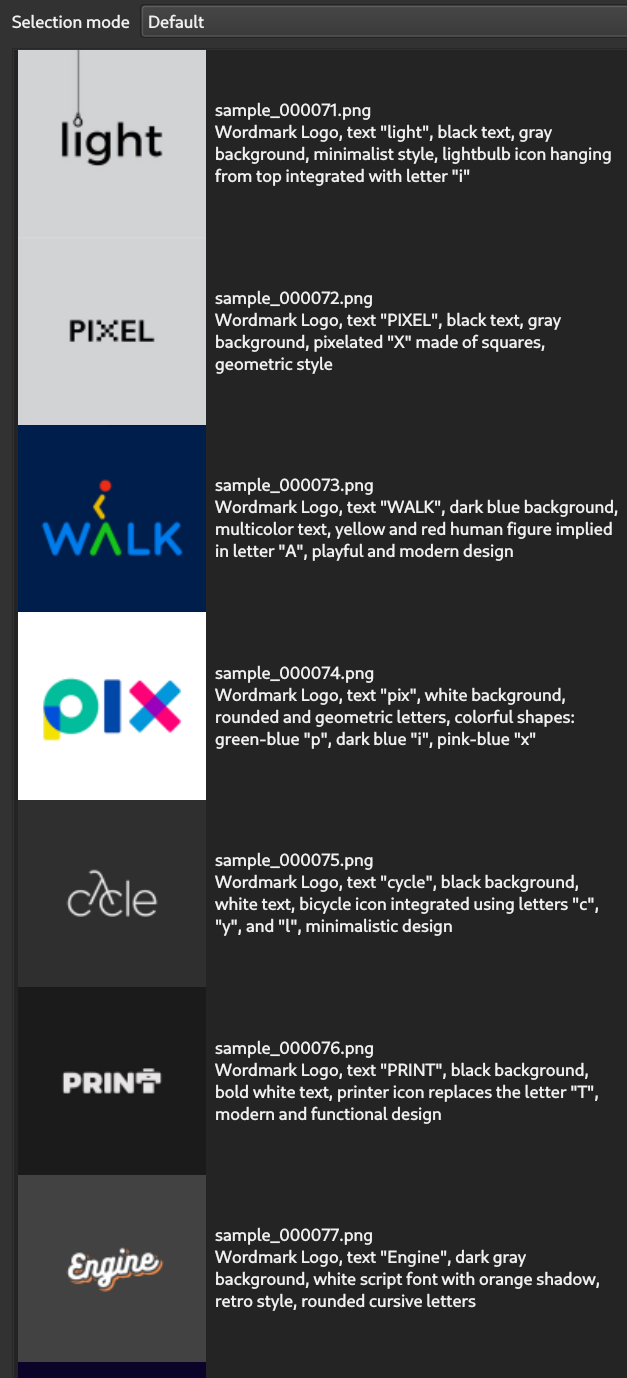
\includegraphics[width=\linewidth]{wordmark.png}
      \caption{wordmark}
    \end{subfigure}
    \begin{subfigure}{0.2\textwidth}
      \centering
      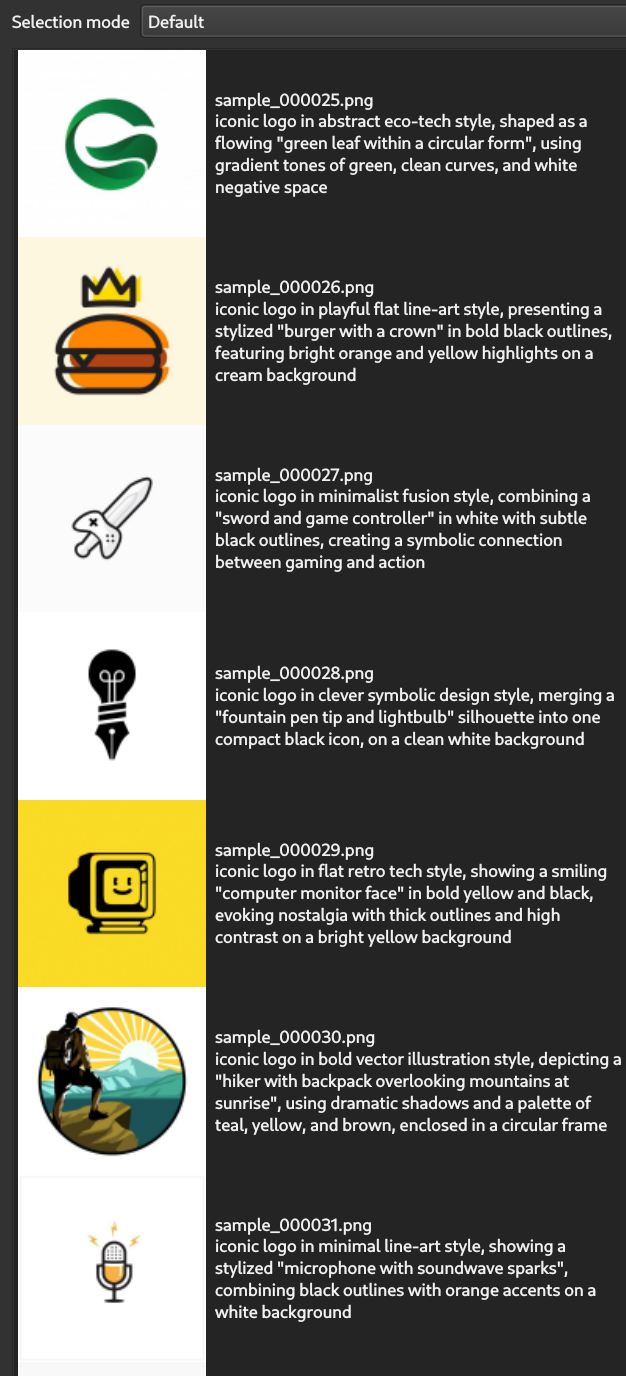
\includegraphics[width=\linewidth]{iconic.png}
      \caption{iconic}
    \end{subfigure}
    \begin{subfigure}{0.2\textwidth}
      \centering
      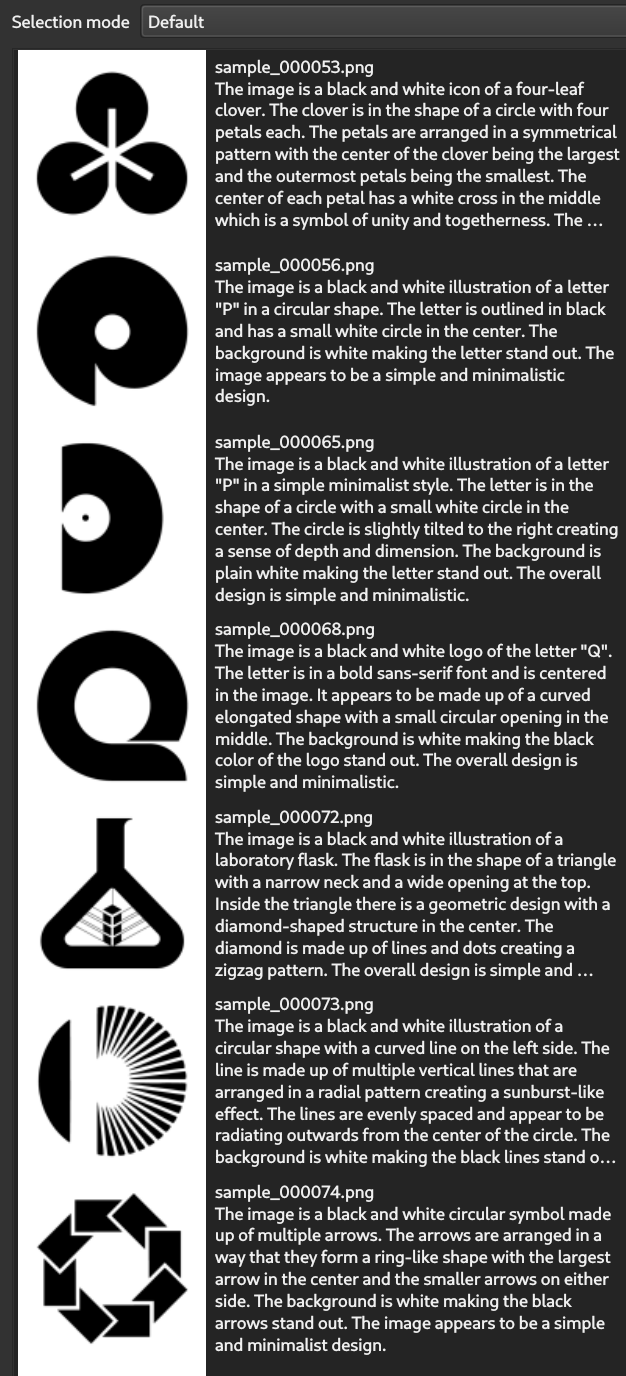
\includegraphics[width=\linewidth]{minimalistic.png}
      \caption{minimalistic}
    \end{subfigure}
    \begin{subfigure}{0.2\textwidth}
      \centering
      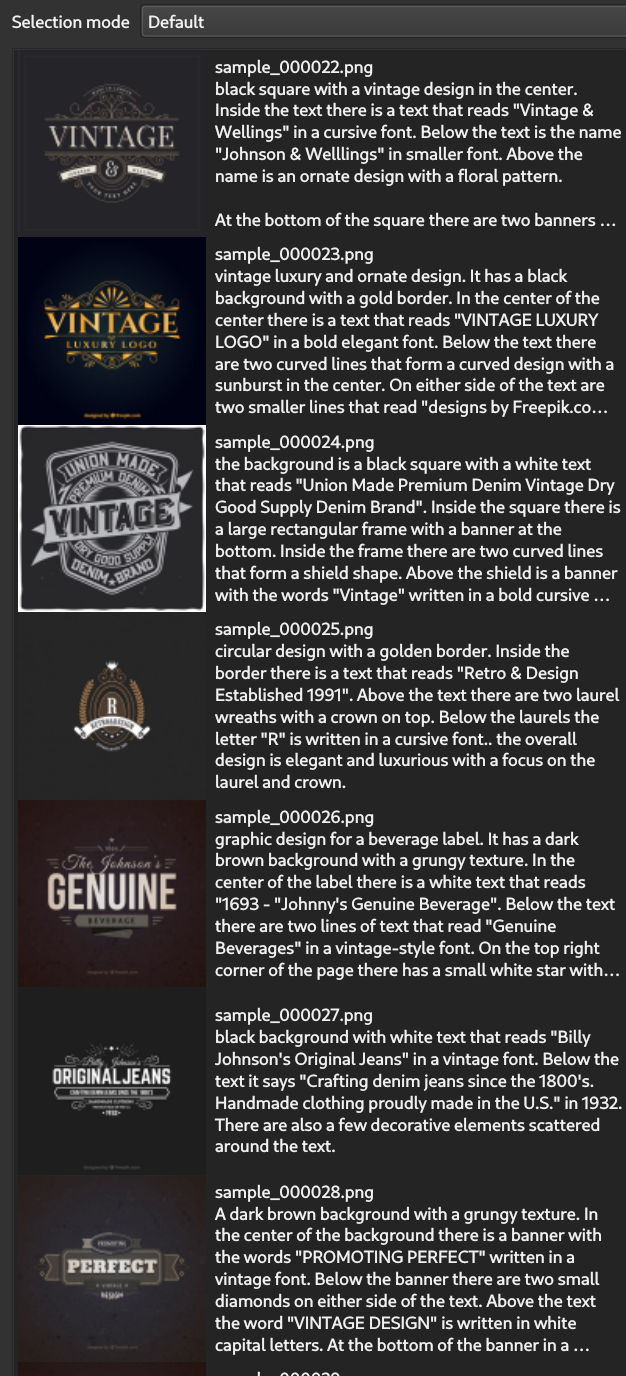
\includegraphics[width=\linewidth]{vintage.png}
      \caption{vintage}
    \end{subfigure}
    \begin{subfigure}{0.2\textwidth}
      \centering
      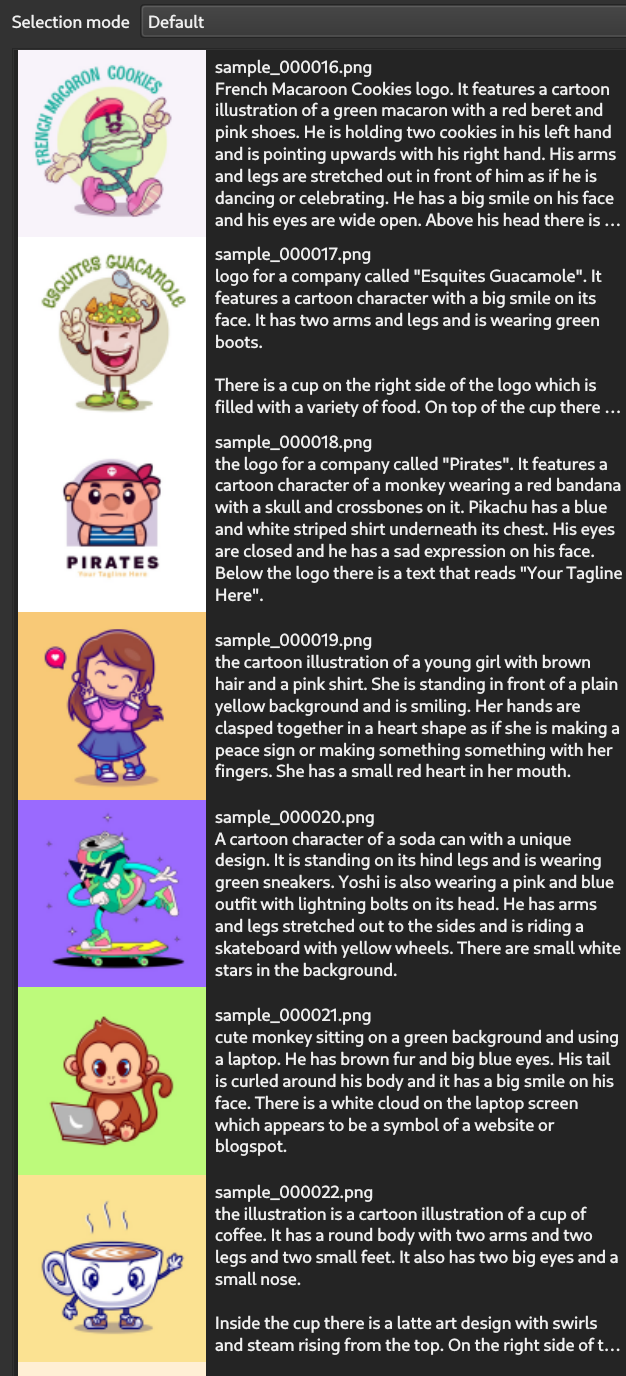
\includegraphics[width=\linewidth]{cartoon.png}
      \caption{cartoon}
    \end{subfigure}
    \caption{Pequenas amostras dos datasets criados.}
\end{figure}

\section{Execução e Ajuste dos Treinamentos com Kohya\_ss}

O treinamento foi realizado no Kohya\_ss, definindo parâmetros específicos para cada dataset após testes experimentais:

\begin{itemize}
    \item \textbf{LR (global).} Taxa de aprendizado base aplicada aos adaptadores LoRA; escala o gradiente em todas as camadas alvo salvo quando sobrescrito pelos valores específicos de \textit{Text LR} ou \textit{UNet LR}.
    \item \textbf{Text LR.} Taxa de aprendizado dedicada às projeções LoRA inseridas no codificador textual (CLIP), regulando a atualização dos pesos das camadas Transformer e dos embeddings de tokens.
    \item \textbf{UNet LR.} Taxa de aprendizado atribuída exclusivamente às camadas LoRA adicionadas ao \textit{UNet} responsáveis pela síntese de imagem.
    \item \textbf{Epoch.} Quantidade de passagens completas pelo conjunto de treinamento; cada época garante que todas as amostras contribuam para a otimização dos parâmetros.
\end{itemize}

\begin{table}[!ht]
    \centering
    \small
    \setlength{\tabcolsep}{4pt}
    \begin{tabularx}{\linewidth}{|X|c|c|c|c|}
    \hline
    \textbf{Dataset} & \textbf{LR} & \textbf{Text LR} & \textbf{UNet LR} & \textbf{Epoch} \\ \hline
    Wordmark               & 0{,}0003 & 0{,}0001 & 0{,}0001 & 10 \\ \hline
    Iconic                 & 0{,}0003 & 0{,}0001 & 0{,}0001 & 10 \\ \hline
    Minimalistic           & 0{,}001  & 0{,}00005 & 0{,}0001 & 10 \\ \hline
    Vintage                & 0{,}001  & 0{,}00005 & 0{,}0001 & 10 \\ \hline
    Cartoon                & 0{,}001  & 0{,}00005 & 0{,}0001 & 10 \\ \hline
    \end{tabularx}
    \caption{Parâmetros empregados nos treinamentos dos LoRAs}
    \label{tab:parametros_lora}
\end{table}

Os parâmetros acima foram escolhidos a fim de reduzir ruído e aumentar a fidelidade visual-textual. Embora taxas de aprendizagem muito baixas sejam a norma, constatei que, nos LoRAs de estilo, foi necessário elevar o LR global para que o modelo incorporasse nuances estéticas sem comprometer a estabilidade.

\section{Implementação dos Fluxos em ComfyUI}

Três fluxos foram desenvolvidos para a geração e estilização automática de logomarcas:

\subsection{Fluxo Text-to-Image (text2img)}

O primeiro fluxo gera a imagem \emph{ex nihilo}, partindo apenas da instrução textual. Ele inicia em um bloco de variáveis que armazena a \textbf{CFG} (\emph{Classifier-Free Guidance}, escala de orientação), a \emph{Seed} aleatória, o número de \emph{Steps} (etapas de remoção de ruído), o tamanho do conjunto de imagens a serem geradas e os textos positivo e negativo. Em seguida, o grafo carrega o \textbf{SDXL Checkpoint} e, opcionalmente, até seis arquivos LoRA que serão injetados no momento da inferência.

Do lado textual, dois nós específicos do SDXL—\textit{Positive Prompt CLIP Text Encode} e \textit{Negative Prompt CLIP Text Encode}—transformam os textos em \emph{embeddings} semânticos pelo CLIP. Esses vetores condicionam o \textbf{KSampler}, que executa o ciclo de \emph{denoising} segundo a agenda de ruído escolhida (DDIM, DPM++ etc.). Ao final das iterações, obtém-se um latente refinado; ele passa pelo nó \textit{VAE Decode}, que reconstrói a imagem no espaço de pixels e a envia ao painel de saída.

\begin{figure}[H]
    \centering
	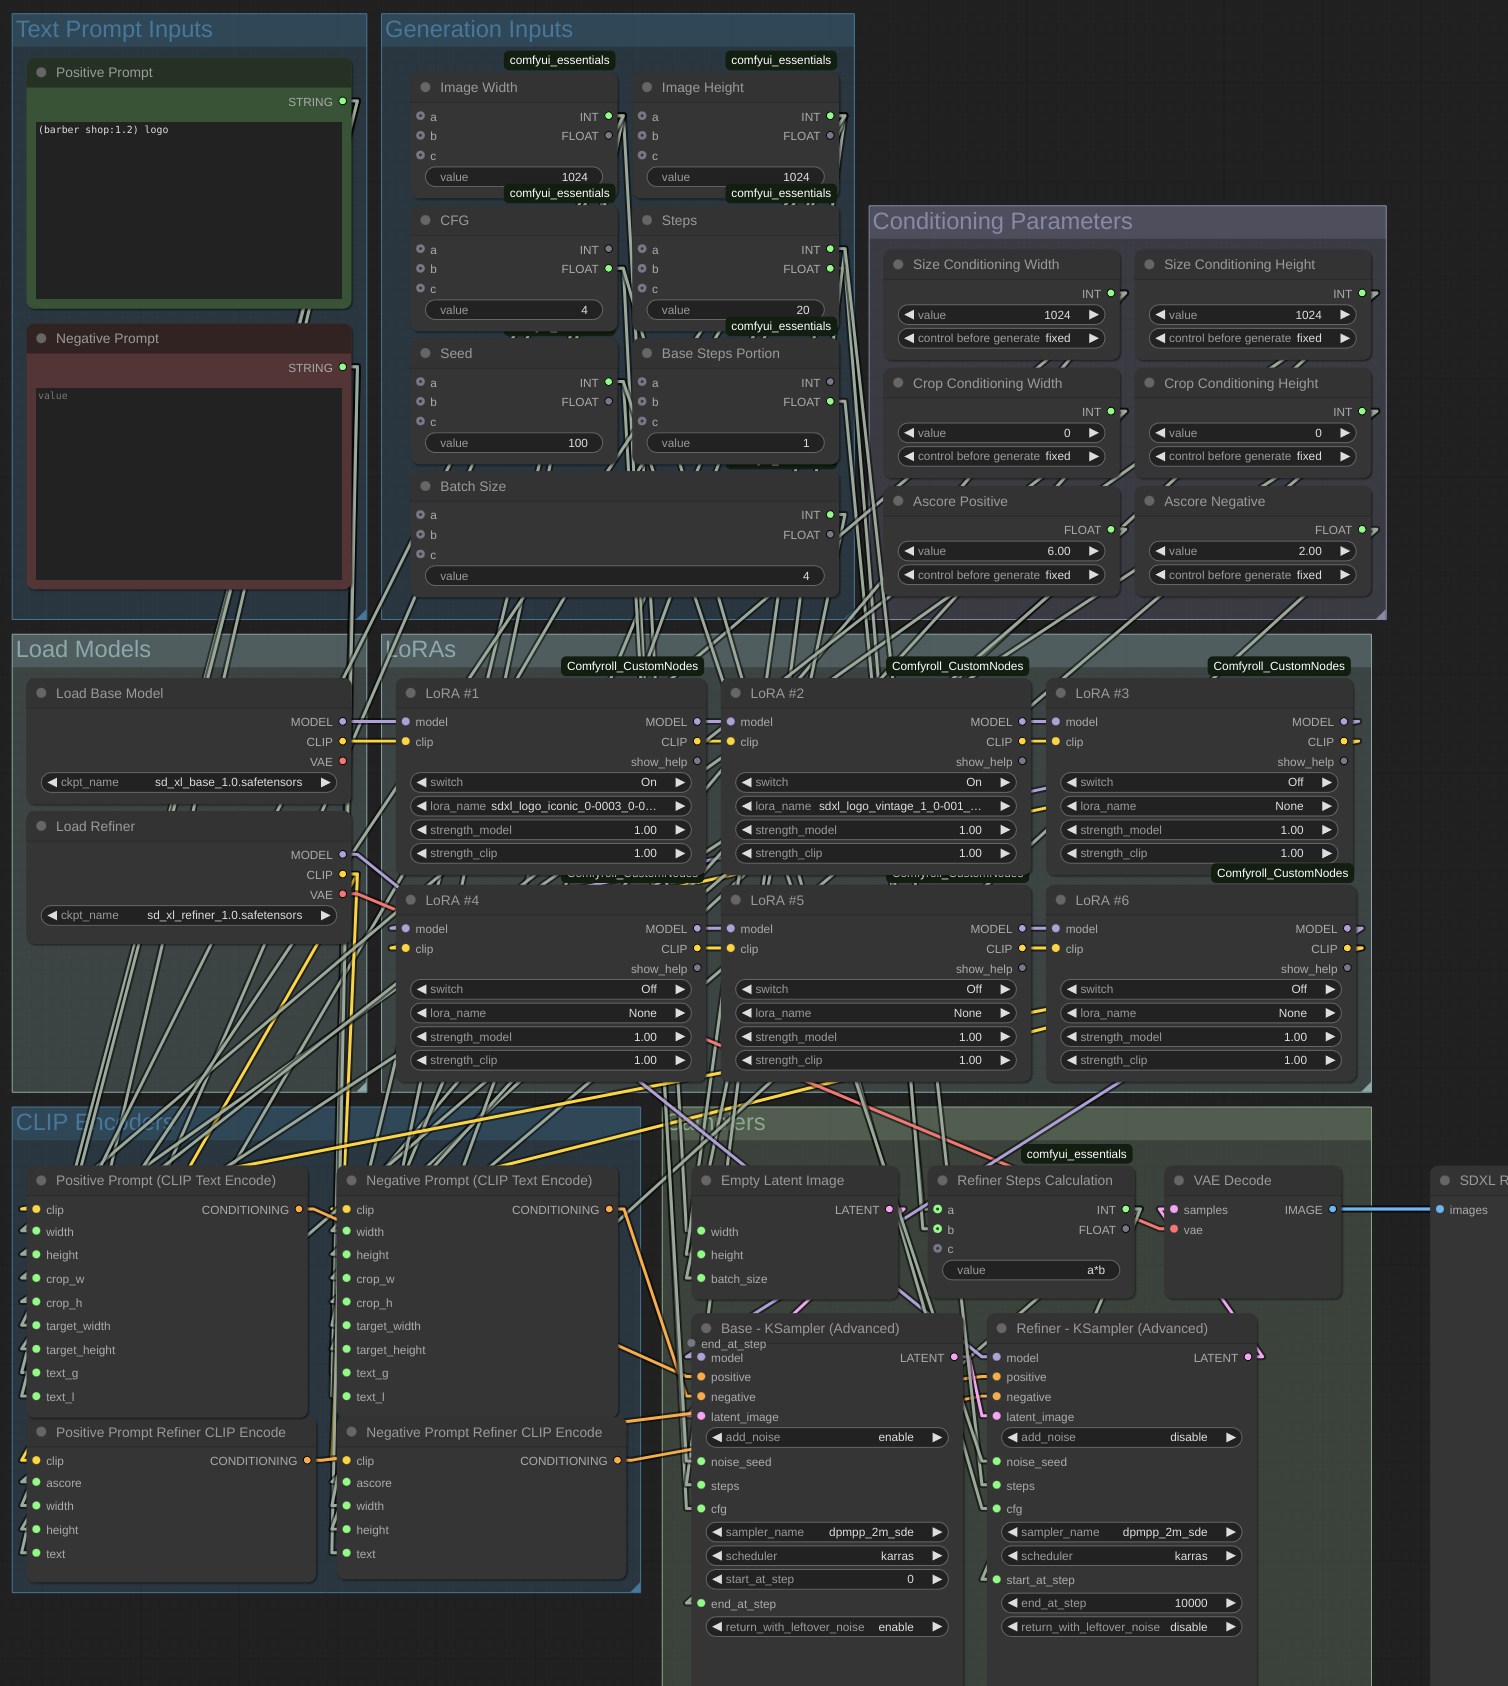
\includegraphics[width=\linewidth]{figuras/text2img-flow.png}
	\caption[Fluxo Text-to-Image (ComfyUI)]{Screenshot do fluxo de Text-to-Image dentro do ComfyUI}
	\label{fig:text2imgFlow}
\end{figure}

\subsection{Fluxo Image-to-Image (img2img)}

O segundo fluxo replica a topologia anterior, mas substitui a amostra de ruído inicial por uma \textbf{imagem base} fornecida pelo usuário. Um parâmetro de ``força de \emph{denoising}'' determina quanta informação visual dessa entrada será preservada. O restante do processo — codificação textual, injeção de LoRAs, amostragem pelo KSampler e decodificação pelo VAE — permanece idêntico. O resultado é uma estilização controlada da imagem original, útil para aplicar temas (\emph{minimalistic}, \emph{vintage}, \emph{cartoon}) mantendo a composição geral.

\begin{figure}[H]
    \centering
	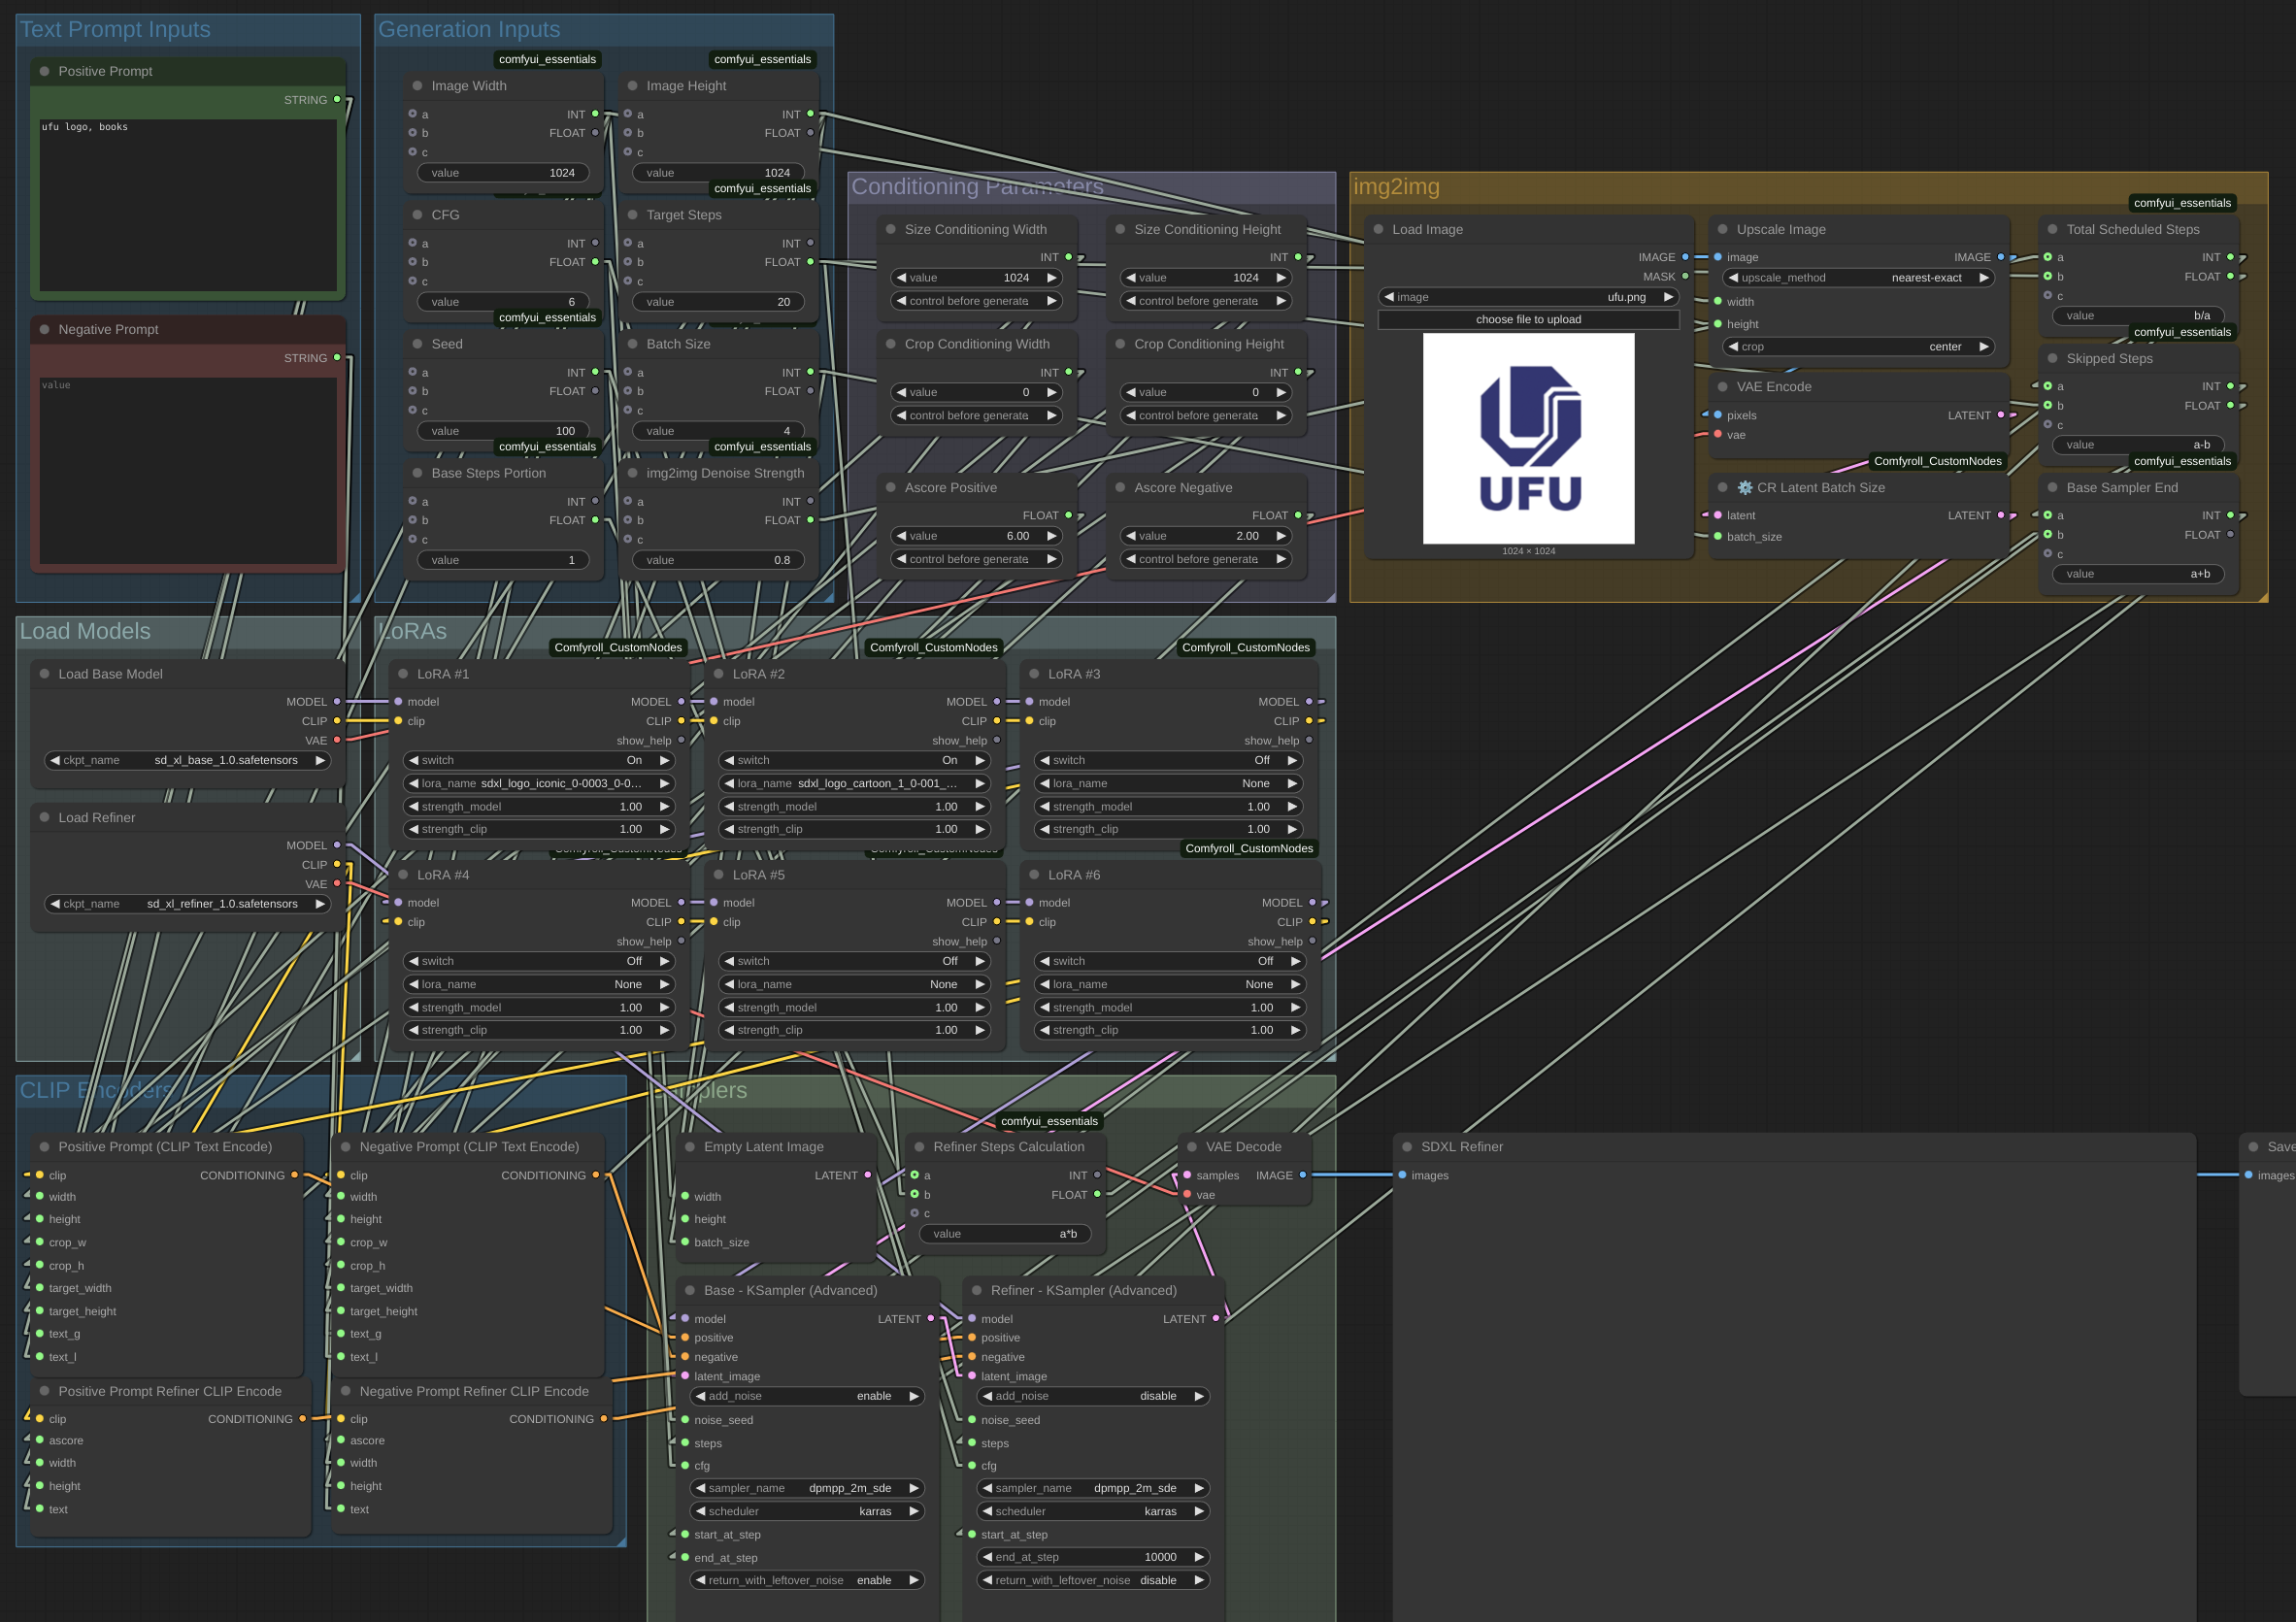
\includegraphics[width=\linewidth]{figuras/img2img-flow.png}
	\caption[Fluxo Image-to-Image (ComfyUI)]{Screenshot do fluxo de Image-to-Image dentro do ComfyUI}
	\label{fig:img2imgFlow}
\end{figure}

\subsection{Fluxo Fix-Text (Correção Textual)}

O terceiro fluxo destina-se a corrigir texto em imagens existentes. Ele começa com a mesma etapa de variáveis globais, mas o condicionamento principal é feito por um \textbf{ControlNet Inpainting}. A imagem de entrada é processada por \textbf{EasyOCR} (ferramenta de reconhecimento óptico de caracteres); qualquer texto detectado é convertido em uma máscara binária que indica as áreas a serem redesenhadas. Essa máscara e a imagem original alimentam o ControlNet, que orienta a U-Net a denoiser apenas as regiões mascaradas, preservando o restante da cena. Após o ciclo de denoising guiado, o latente volta ao \textit{VAE Decode}, resultando em uma versão corrigida onde o texto foi reescrito de forma mais legível e integrada ao contexto visual.

\begin{figure}[H]
    \centering
	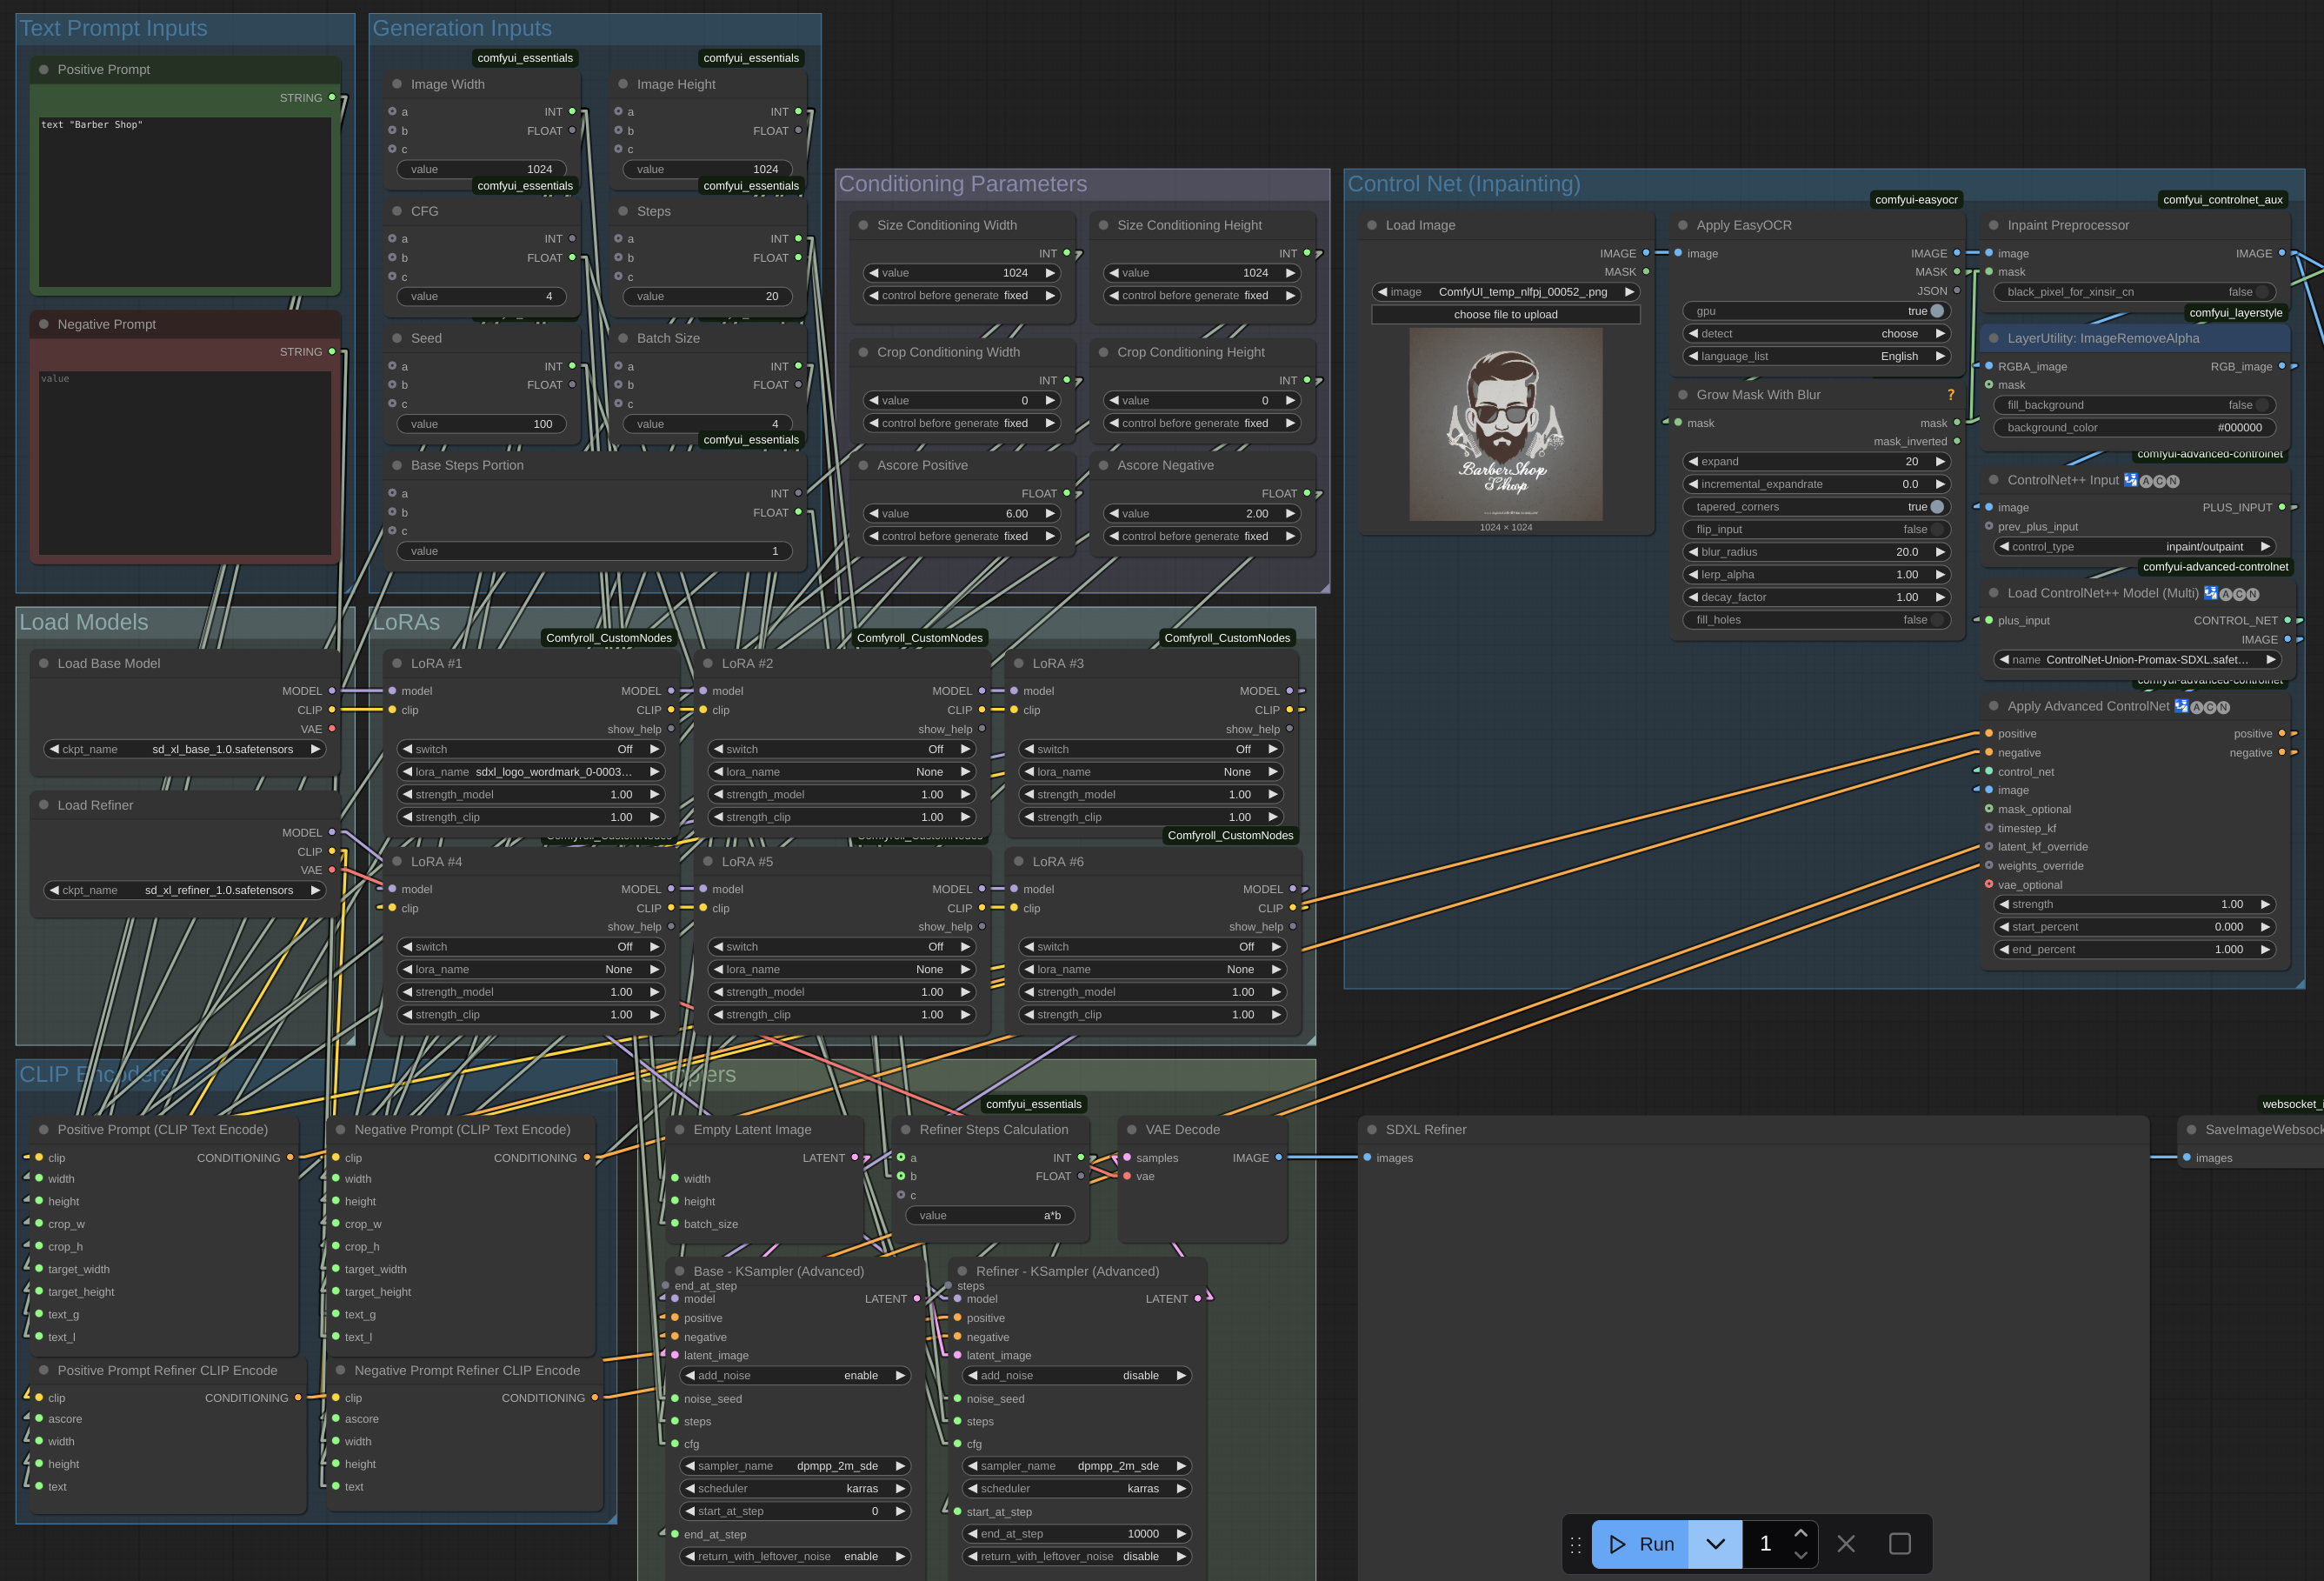
\includegraphics[width=\linewidth]{figuras/fix-text-flow.png}
	\caption[Fluxo Fix-Text (ComfyUI)]{Screenshot do fluxo de Fix-Text dentro do ComfyUI}
	\label{fig:fixTextFlow}
\end{figure}

\section{Planejamento e Execução da Avaliação Experimental}

Para avaliar os LoRAs, 30 instruções textuais foram criadas para cada tipo básico de logomarca, com variações de estilo, CFG e Steps:

\begin{itemize}
    \item 60 instruções textuais únicas (acessíveis \href{https://github.com/tornellihenrique/tcc-stable-diffusion-logos/tree/main/result-gathering/prompts}{neste endereço})
    \item 3 estilos: Minimalistic, Vintage, Cartoon
    \item CFG: 4.0, 5.0, 6.0
    \item Steps: 15, 20, 25
    \item Algoritmo de Amostragem e Agenda de Ruído: DPM++ 2M SDE Karras
    \item Batches de 4 imagens cada, totalizando 8\,640 imagens únicas geradas
\end{itemize}

\section{Análise de Resultados e Métricas}

Após o processo de geração de imagens, foram criadas algumas imagens de comparação que contêm as imagens geradas. O objetivo é identificar as logomarcas mais apropriadas com base no CFG, no número de Steps, no Índice de Batch e no uso do LoRA.

\subsection{Estudo de Caso Inicial}

Comparação produzida a partir da mesma instrução textual apresentada inicialmente para demonstrar o problema. Essa amostra-guia ilustra, lado a lado, a saída \textit{baseline} do SDXL (Sem LoRA) e as variantes geradas com LoRA e configuração explorada (CFG, Steps e índice de batch).

\begin{figure}[H]
    \centering
	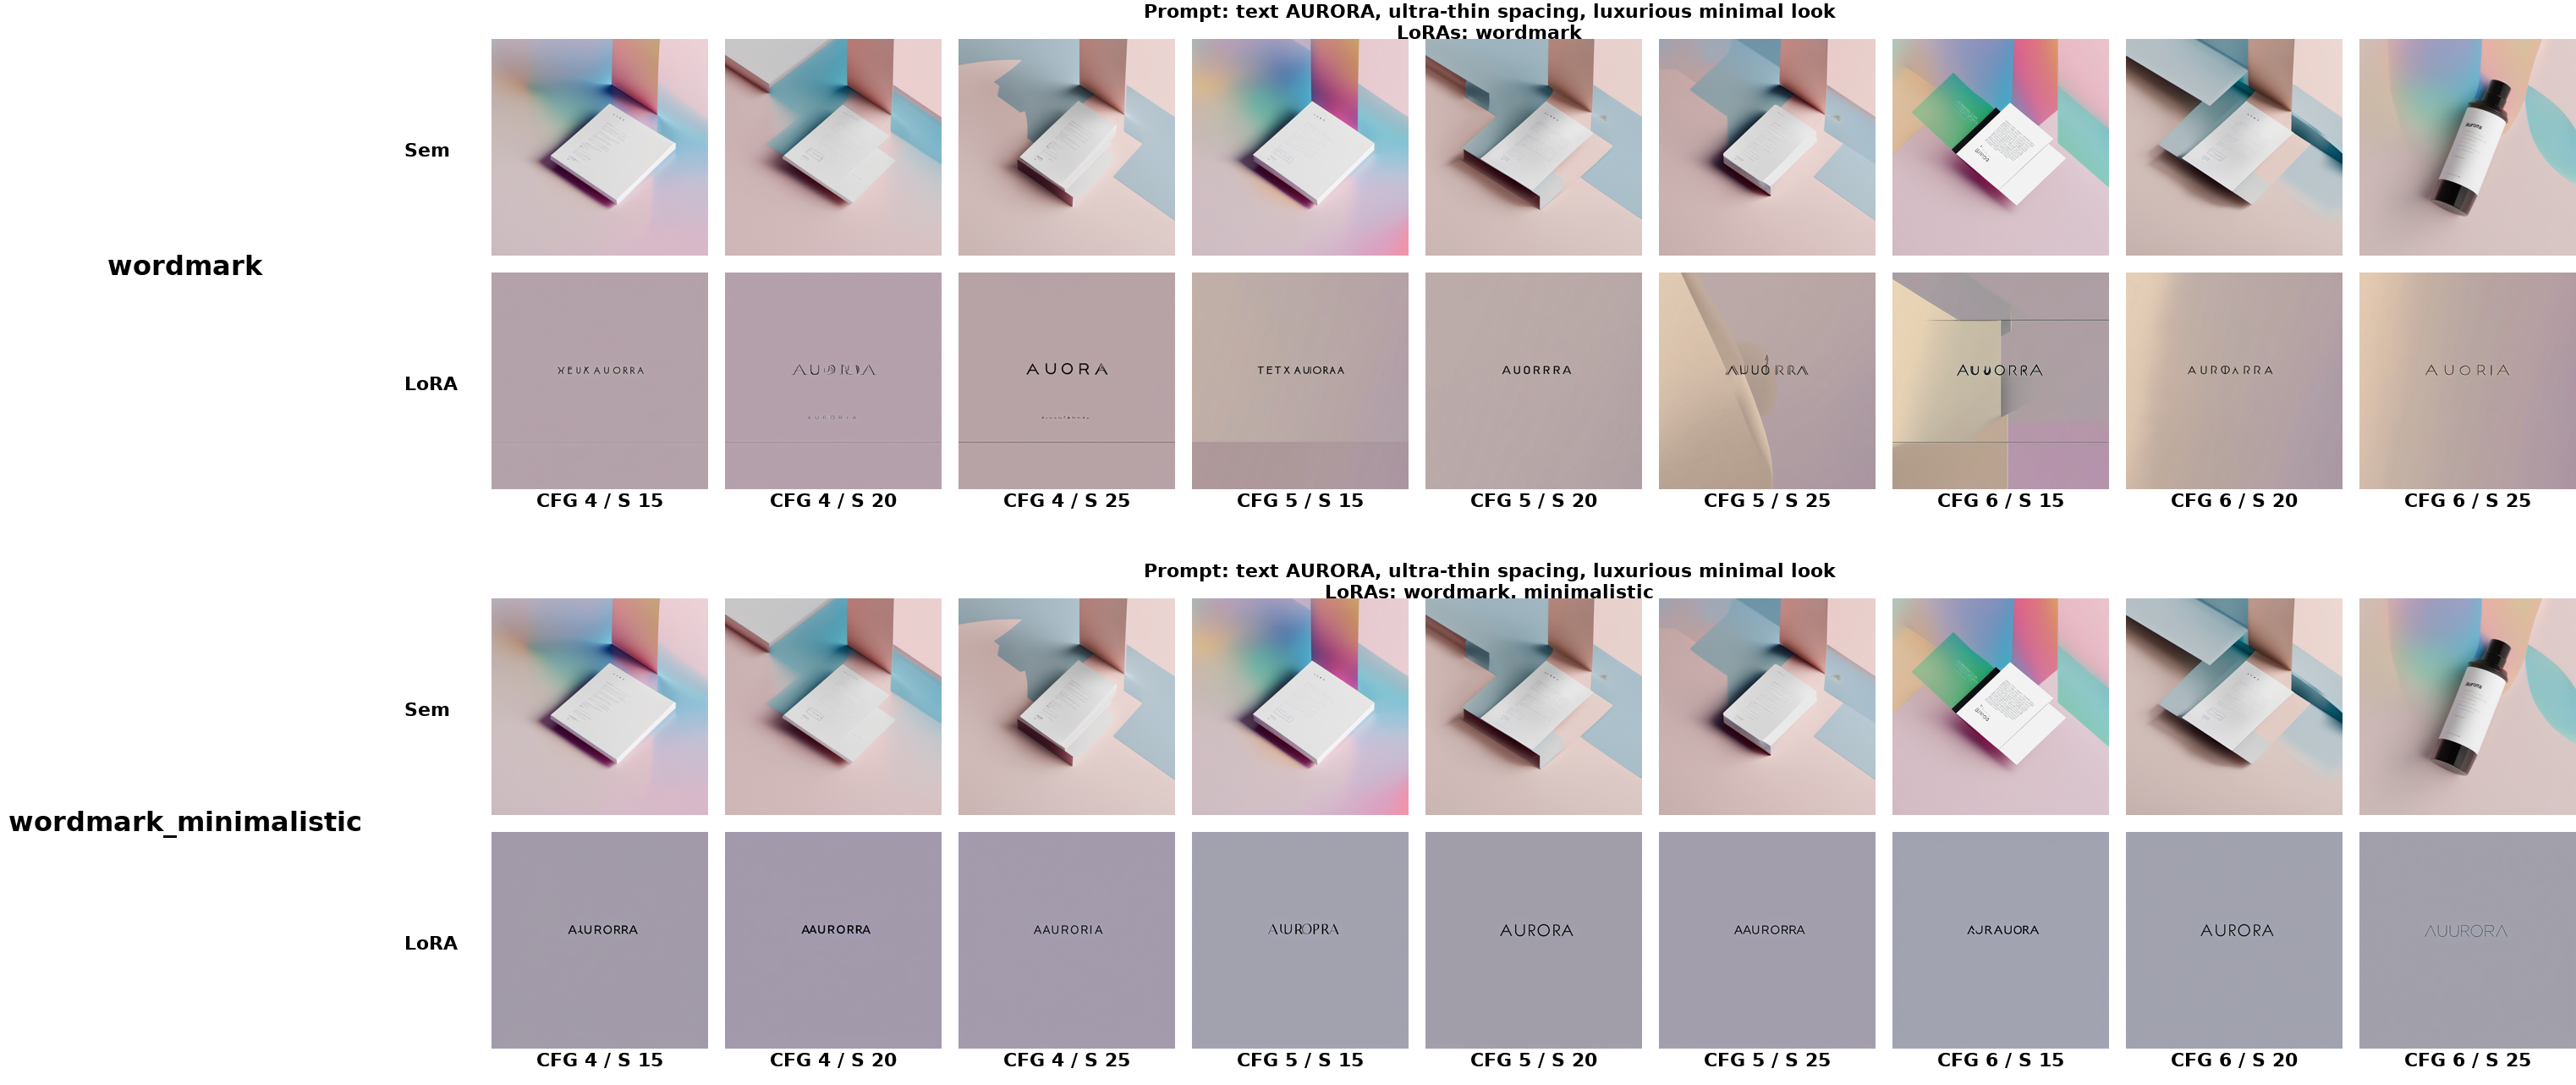
\includegraphics[width=\linewidth]{figuras/resultados/good/wordmark/cmp_p2_batch1.png}
	\caption[Primeira comparação das saídas sem e com os LoRAs criados, a partir do prompt ``AURORA''.]{Primeira comparação das saídas sem e com os LoRAs criados, a partir do prompt: text AURORA, ultra-thin spacing, luxurious minimal look}
	\label{fig:cmpP2Batch1}
\end{figure}

\begin{figure}[H]
    \centering
	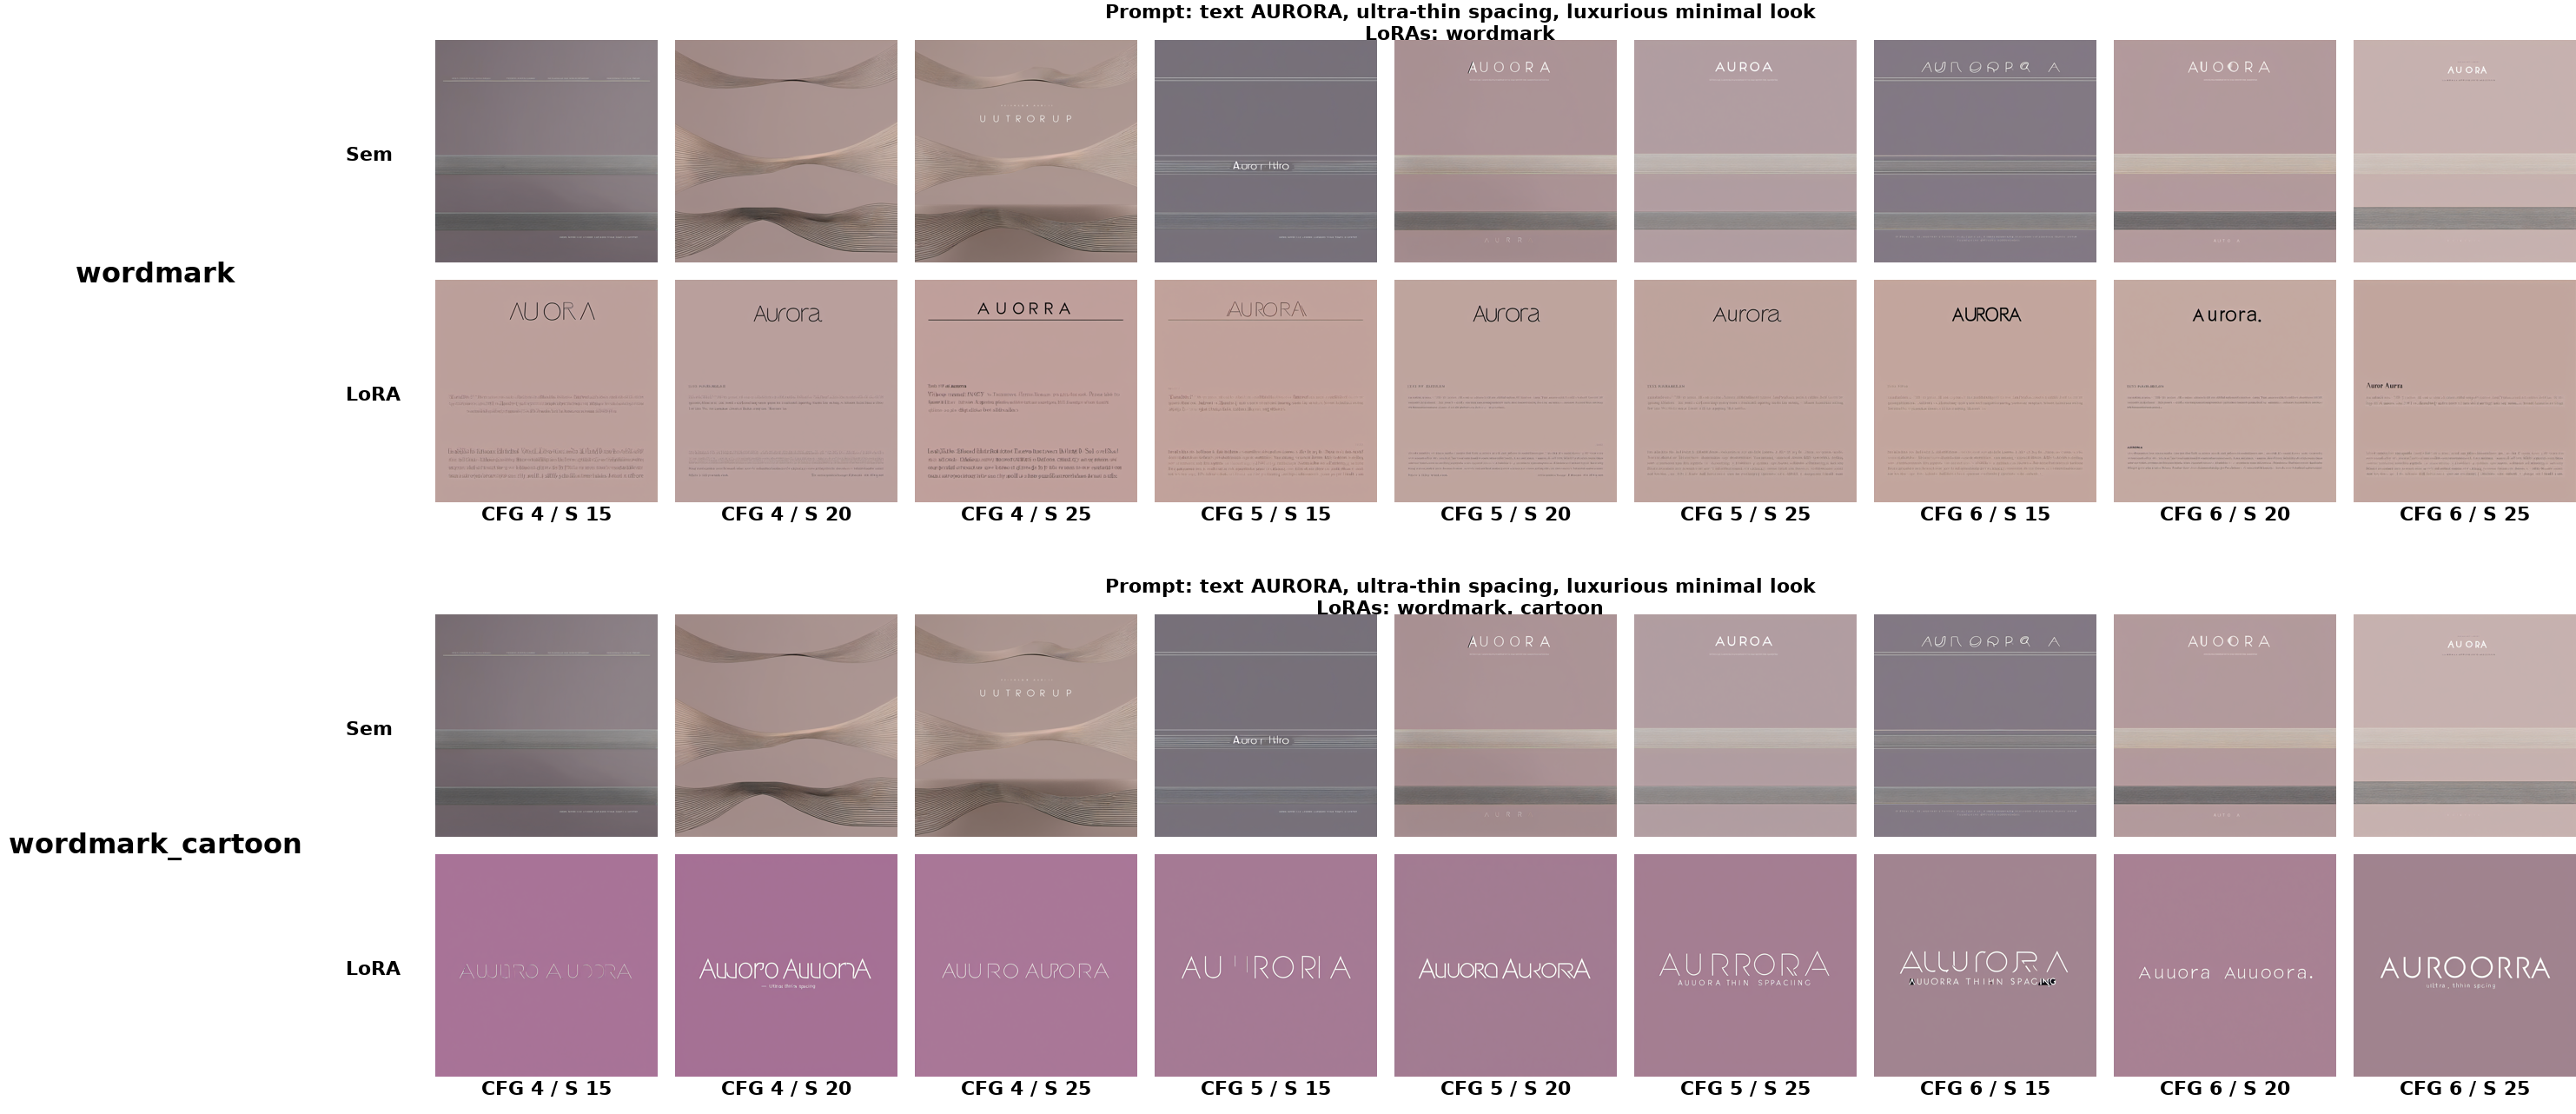
\includegraphics[width=\linewidth]{figuras/resultados/good/wordmark/cmp_p2_batch3.png}
	\caption[Segunda comparação das saídas sem e com os LoRAs criados, a partir do prompt ``AURORA''.]{Segunda comparação das saídas sem e com os LoRAs criados, a partir do prompt: text AURORA, ultra-thin spacing, luxurious minimal look}
	\label{fig:cmpP2Batch3}
\end{figure}

\subsection{Resultados Gerais}

Em seguida são apresentados os painéis de comparação completos, englobando alguns exemplos dentre as 8\,640 imagens obtidas. Os gráficos e tabelas sintetizam o impacto de cada parâmetro (CFG, Steps, batch e uso de LoRA) nas métricas de legibilidade, fidelidade de estilo e consistência visual.

\begin{figure}[H]
    \centering
    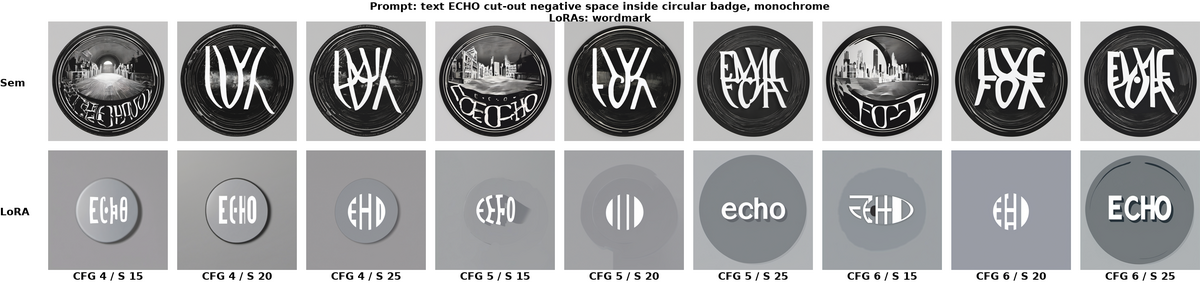
\includegraphics[width=1.0\linewidth]{figuras/resultados/good/wordmark/p7_batch0.png}
    \caption[1º Comparação das saídas sem e com o LoRA criado.]{Comparação das saídas sem e com o LoRA criado. Prompt: text ECHO cut-out negative space inside circular badge, monochrome}
    \label{fig:wordmarkP7Batch0}
\end{figure}

\begin{figure}[H]
    \centering
    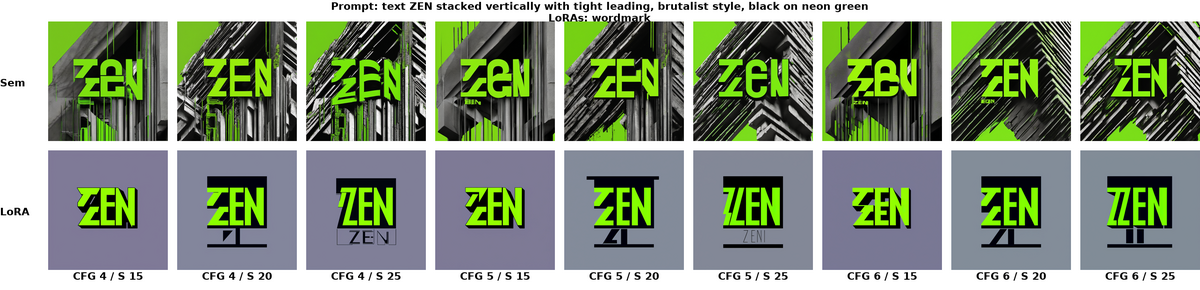
\includegraphics[width=1.0\linewidth]{figuras/resultados/good/wordmark/p5_batch1.png}
    \caption[2º Comparação das saídas sem e com o LoRA criado.]{Comparação das saídas sem e com o LoRA criado. Prompt: text ZEN stacked vertically with tight leading, brutalist style, bacl on neon green}
    \label{fig:wordmarkP5Batch1}
\end{figure}

\begin{figure}[H]
    \centering
    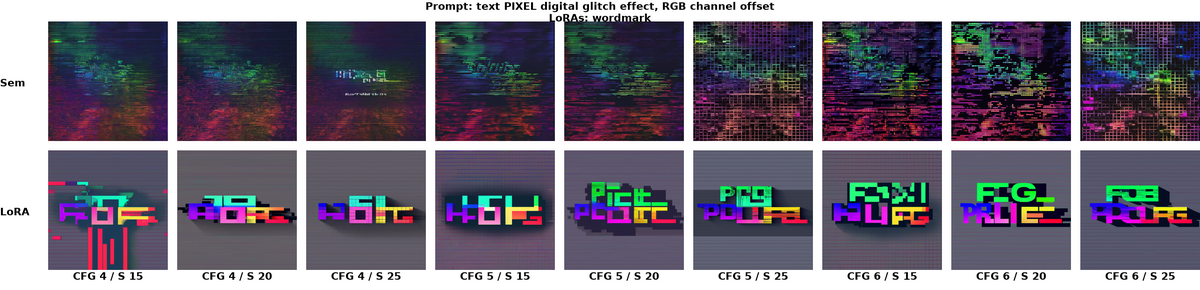
\includegraphics[width=1.0\linewidth]{figuras/resultados/good/wordmark/p18_batch0.png}
    \caption[3º Comparação das saídas sem e com o LoRA criado.]{Comparação das saídas sem e com o LoRA criado. Prompt: text PIXEL digital glitch effect, RGB channel offset}
    \label{fig:wordmarkP18Batch0}
\end{figure}

\begin{figure}[H]
    \centering
    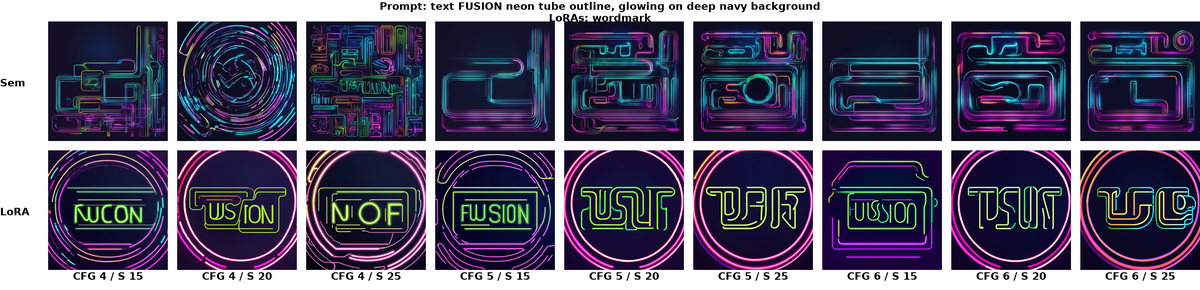
\includegraphics[width=1.0\linewidth]{figuras/resultados/good/wordmark/p23_batch1.png}
    \caption[4º Comparação das saídas sem e com o LoRA criado.]{Comparação das saídas sem e com o LoRA criado. Prompt: text FUSION neon tube outline, glowing on deep navy background}
    \label{fig:wordmarkP23Batch1}
\end{figure}

\begin{figure}[H]
    \centering
    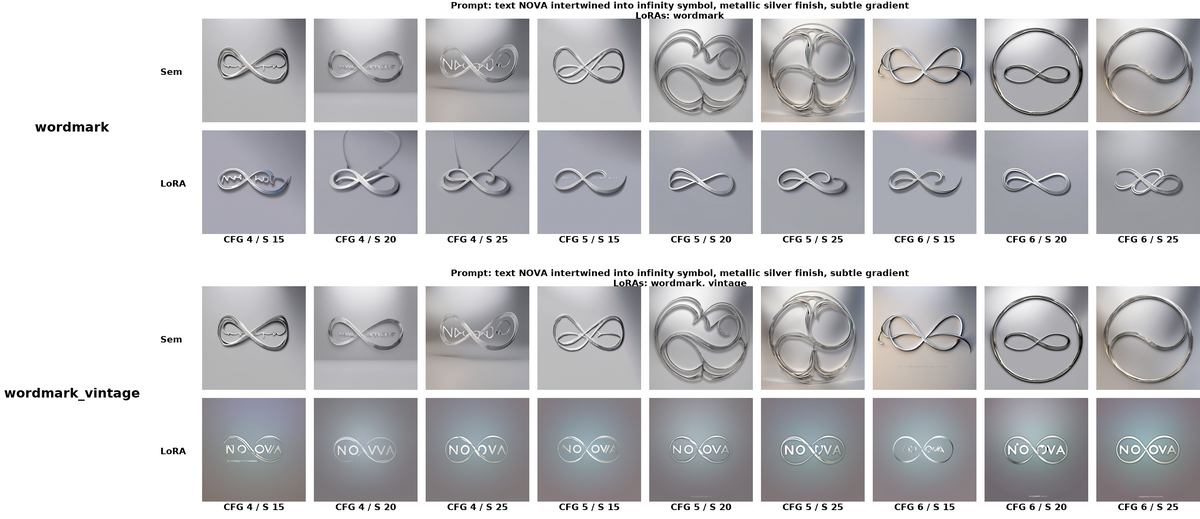
\includegraphics[width=1.0\linewidth]{figuras/resultados/good/wordmark/cmp_p3_batch0.png}
    \caption[5º Comparação das saídas sem e com os LoRAs criados.]{Comparação das saídas sem e com os LoRAs criados. Prompt: text NOVA intertwined into infinity symbol, metallic silver finish, subtle gradient}
    \label{fig:wordmarkCmpP3Batch0}
\end{figure}

\begin{figure}[H]
    \centering
    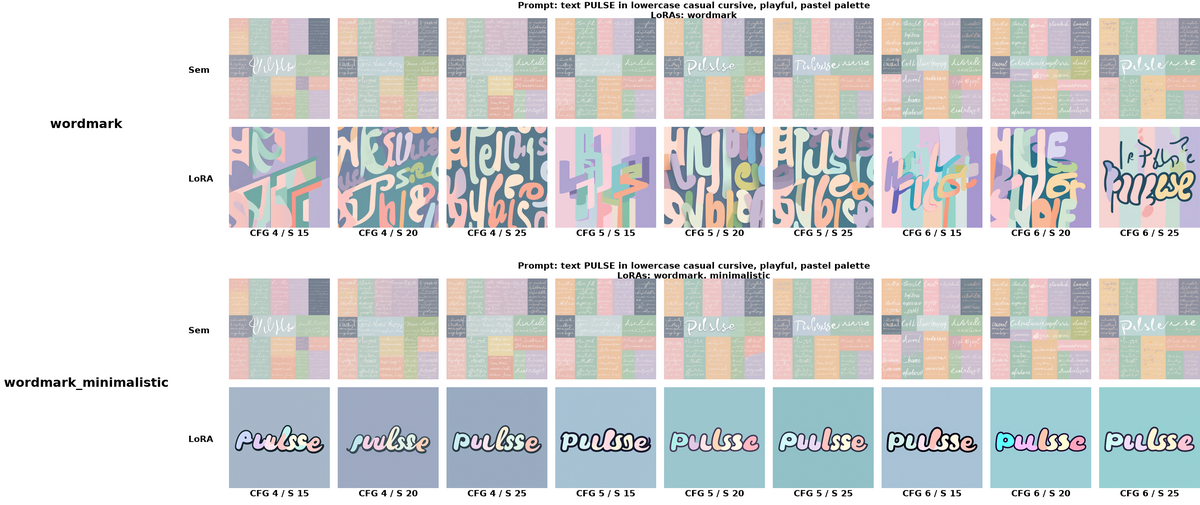
\includegraphics[width=1.0\linewidth]{figuras/resultados/good/wordmark/cmp_p4_batch0.png}
    \caption[6º Comparação das saídas sem e com os LoRAs criados.]{Comparação das saídas sem e com os LoRAs criados. Prompt: text PULSE in lowercase casual cursive, playful, pastel palette}
    \label{fig:wordmarkCmpP4Batch0}
\end{figure}

\begin{figure}[H]
    \centering
    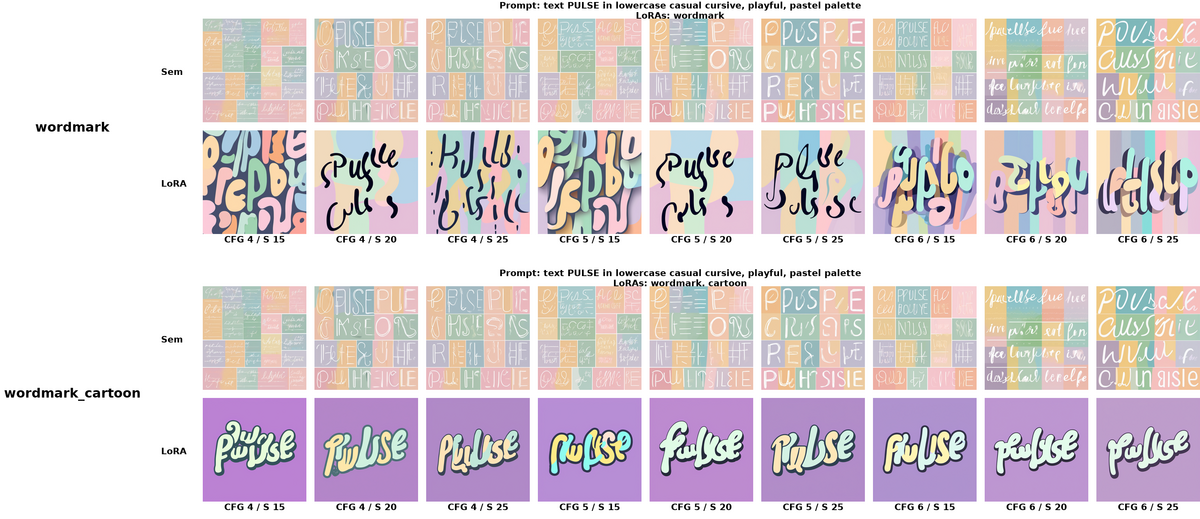
\includegraphics[width=1.0\linewidth]{figuras/resultados/good/wordmark/cmp_p4_batch1.png}
    \caption[7º Comparação das saídas sem e com os LoRAs criados.]{Comparação das saídas sem e com os LoRAs criados. Prompt: text PULSE in lowercase casual cursive, playful, pastel palette}
    \label{fig:wordmarkCmpP4Batch1}
\end{figure}

\begin{figure}[H]
    \centering
    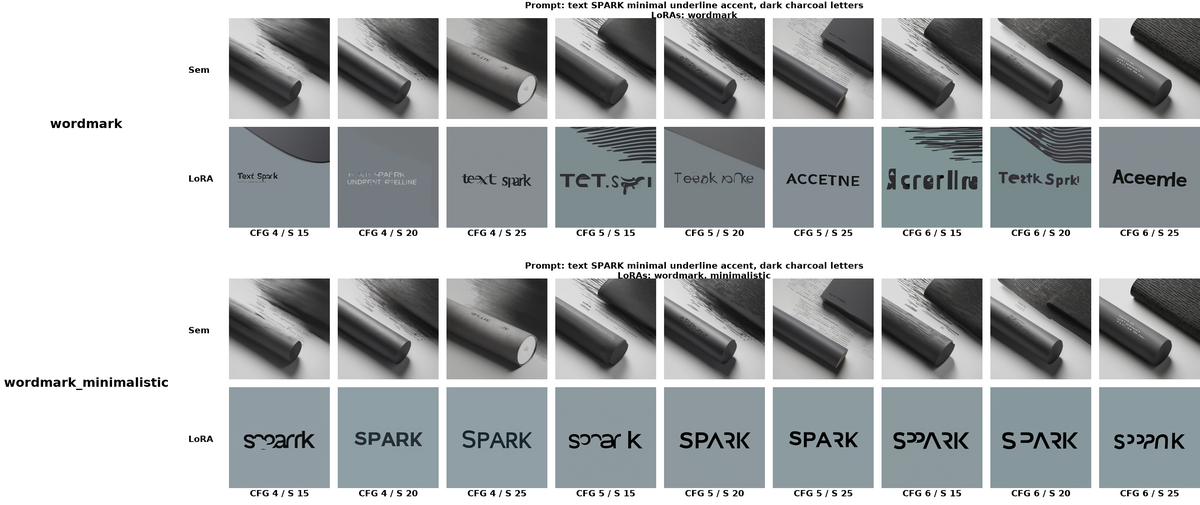
\includegraphics[width=1.0\linewidth]{figuras/resultados/good/wordmark/cmp_p28_batch0.png}
    \caption[8º Comparação das saídas sem e com os LoRAs criados.]{Comparação das saídas sem e com os LoRAs criados. Prompt: text SPARK minimal underline accent, dark charcoal letters}
    \label{fig:wordmarkCmpP28Batch0}
\end{figure}

\begin{figure}[H]
    \centering
    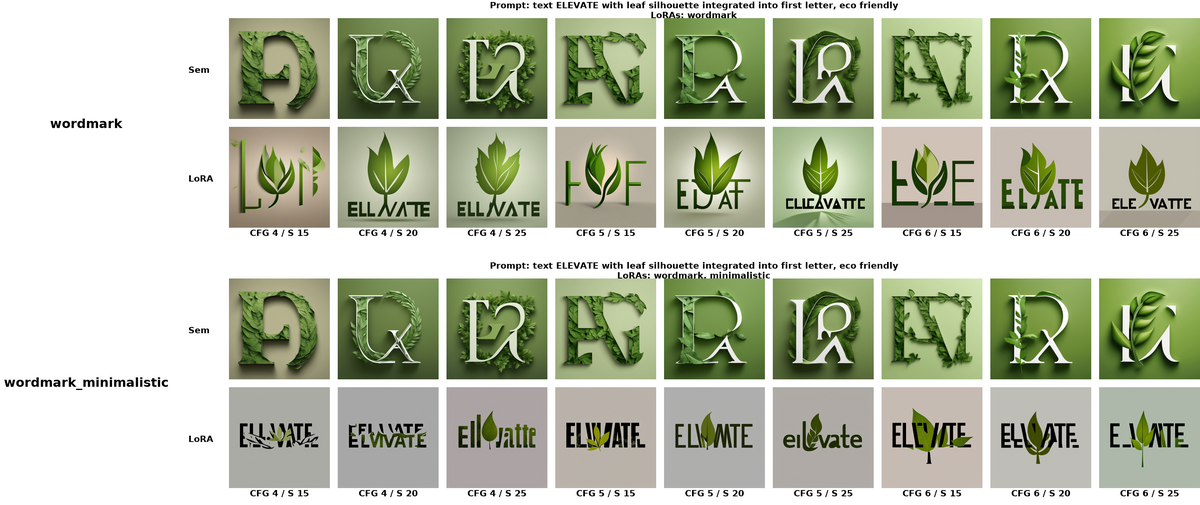
\includegraphics[width=1.0\linewidth]{figuras/resultados/good/wordmark/cmp_p20_batch3.png}
    \caption[9º Comparação das saídas sem e com os LoRAs criados.]{Comparação das saídas sem e com os LoRAs criados. Prompt: text ELEVATE with leaf silhouette integrated into first letter, eco friendly}
    \label{fig:wordmarkCmpP20Batch3}
\end{figure}

\begin{figure}[H]
    \centering
    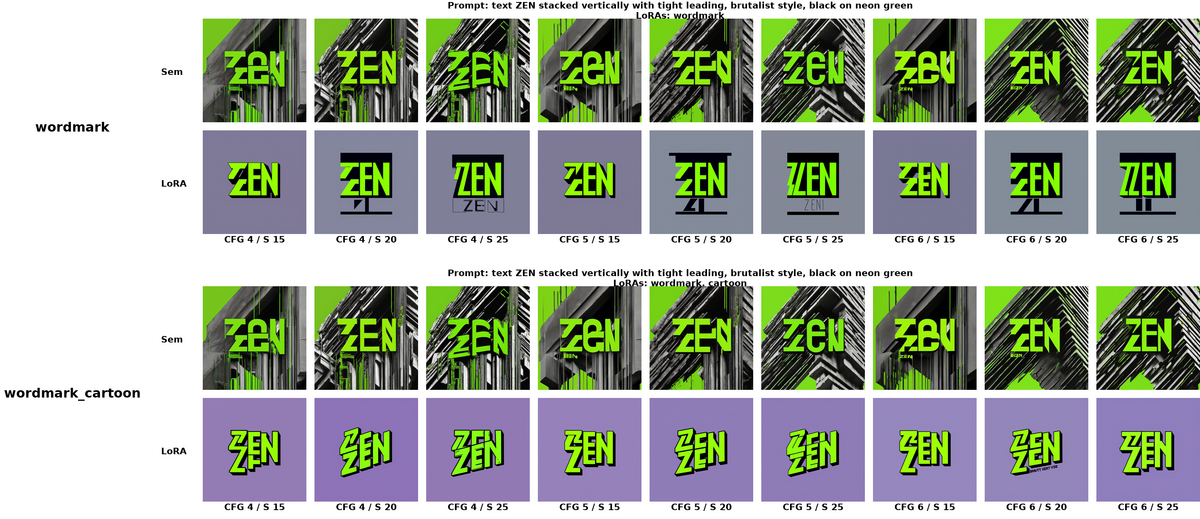
\includegraphics[width=1.0\linewidth]{figuras/resultados/good/wordmark/cmp_p5_batch1.png}
    \caption[10º Comparação das saídas sem e com os LoRAs criados.]{Comparação das saídas sem e com os LoRAs criados. Prompt: text ZEN stacked vertically with tight leading, brutalist style, black on neon green}
    \label{fig:wordmarkCmpP5Batch1}
\end{figure}

\subsection{Análise Visual}

A análise visual dos painéis comprova, de maneira objetiva, o impacto do ajuste fino com LoRA. Nas amostras geradas sem adaptação, o modelo frequentemente deriva: surgem símbolos genéricos, manchas abstratas ou composições que pouco lembram uma logomarca. Após a aplicação dos LoRAs — especialmente na combinação de um LoRA base com um LoRA de estilo — o comportamento torna-se notavelmente mais dirigido. As imagens passam a exibir estrutura centralizada, áreas de respiro equilibradas e paletas cromáticas coerentes, mesmo quando a instrução textual permanece concisa.

A evolução tipográfica é igualmente nítida. Antes, caracteres apareciam distorcidos, duplicados ou ausentes; com o LoRA, o texto não apenas se mantém presente, mas incorpora o estilo proposto—linhas limpas no minimalista, pátina suave no vintage ou contornos expressivos no cartoon. Embora ainda existam pequenas imperfeições, a frequência de falhas severas diminui drasticamente. Em síntese, o LoRA atua como um orientador de arte: mesmo com descrições breves, o modelo entrega logomarcas consistentes e visualmente profissionais, reduzindo a necessidade de ajustes extensos na instrução textual.

\subsection{Resultados Ruins}

Abaixo alguns exemplos que não ficaram bons, para entendermos onde o método falhou.

\begin{figure}[H]
    \centering
    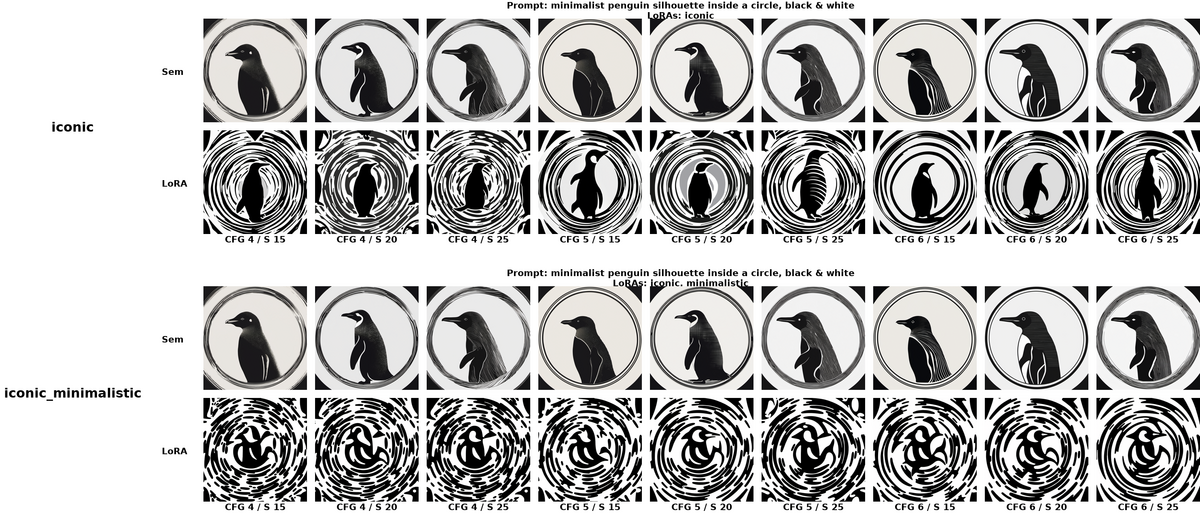
\includegraphics[width=1.0\linewidth]{figuras/resultados/bad/cmp_p1_batch2.png}
    \caption[1º Comparação das saídas ruíns sem e com os LoRAs criados.]{Comparação das saídas ruíns sem e com os LoRAs criados. Prompt: minimalisti penquin silhouette inside a circle, black \& white}
    \label{fig:badCmpP1Batch2}
\end{figure}

\begin{figure}[H]
    \centering
    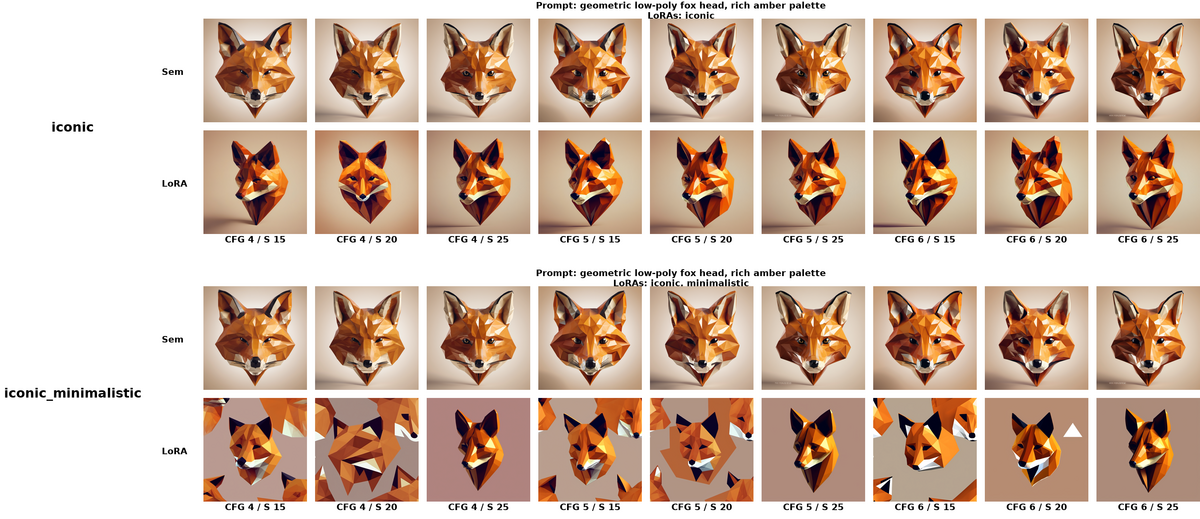
\includegraphics[width=1.0\linewidth]{figuras/resultados/bad/cmp_p5_batch1.png}
    \caption[2º Comparação das saídas ruíns sem e com os LoRAs criados.]{Comparação das saídas ruíns sem e com os LoRAs criados. Prompt: geometric low-poly fox head, rich amber palette}
    \label{fig:badCmpP5Batch1}
\end{figure}

\begin{figure}[H]
    \centering
    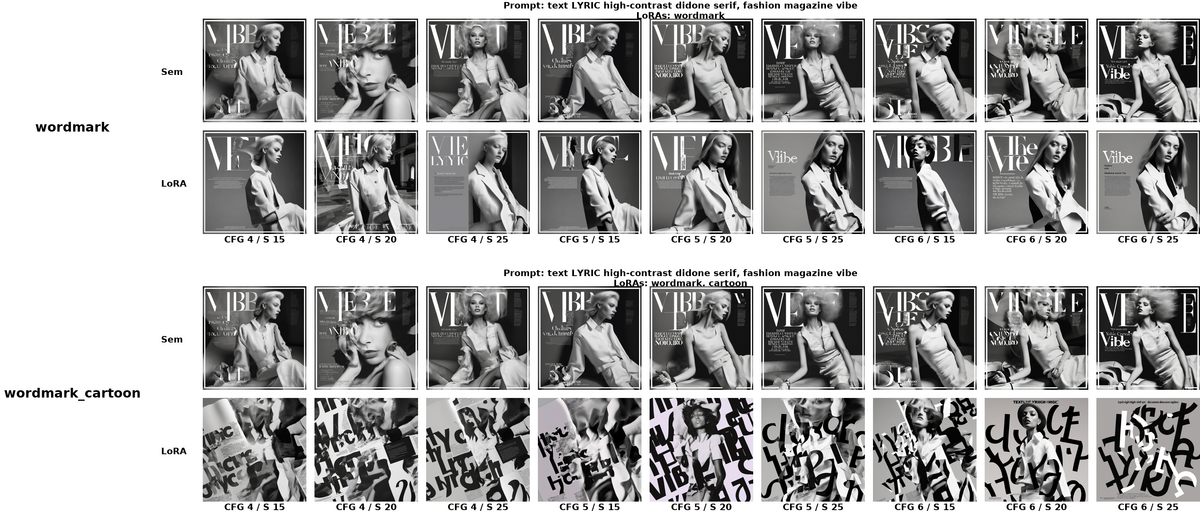
\includegraphics[width=1.0\linewidth]{figuras/resultados/bad/cmp_p26_batch0.png}
    \caption[3º Comparação das saídas ruíns sem e com os LoRAs criados.]{Comparação das saídas ruíns sem e com os LoRAs criados. Prompt: text LYRIC high-contrast didone serif, fashion magazine vibe}
    \label{fig:badCmpP26Batch0}
\end{figure}

\begin{figure}[H]
    \centering
    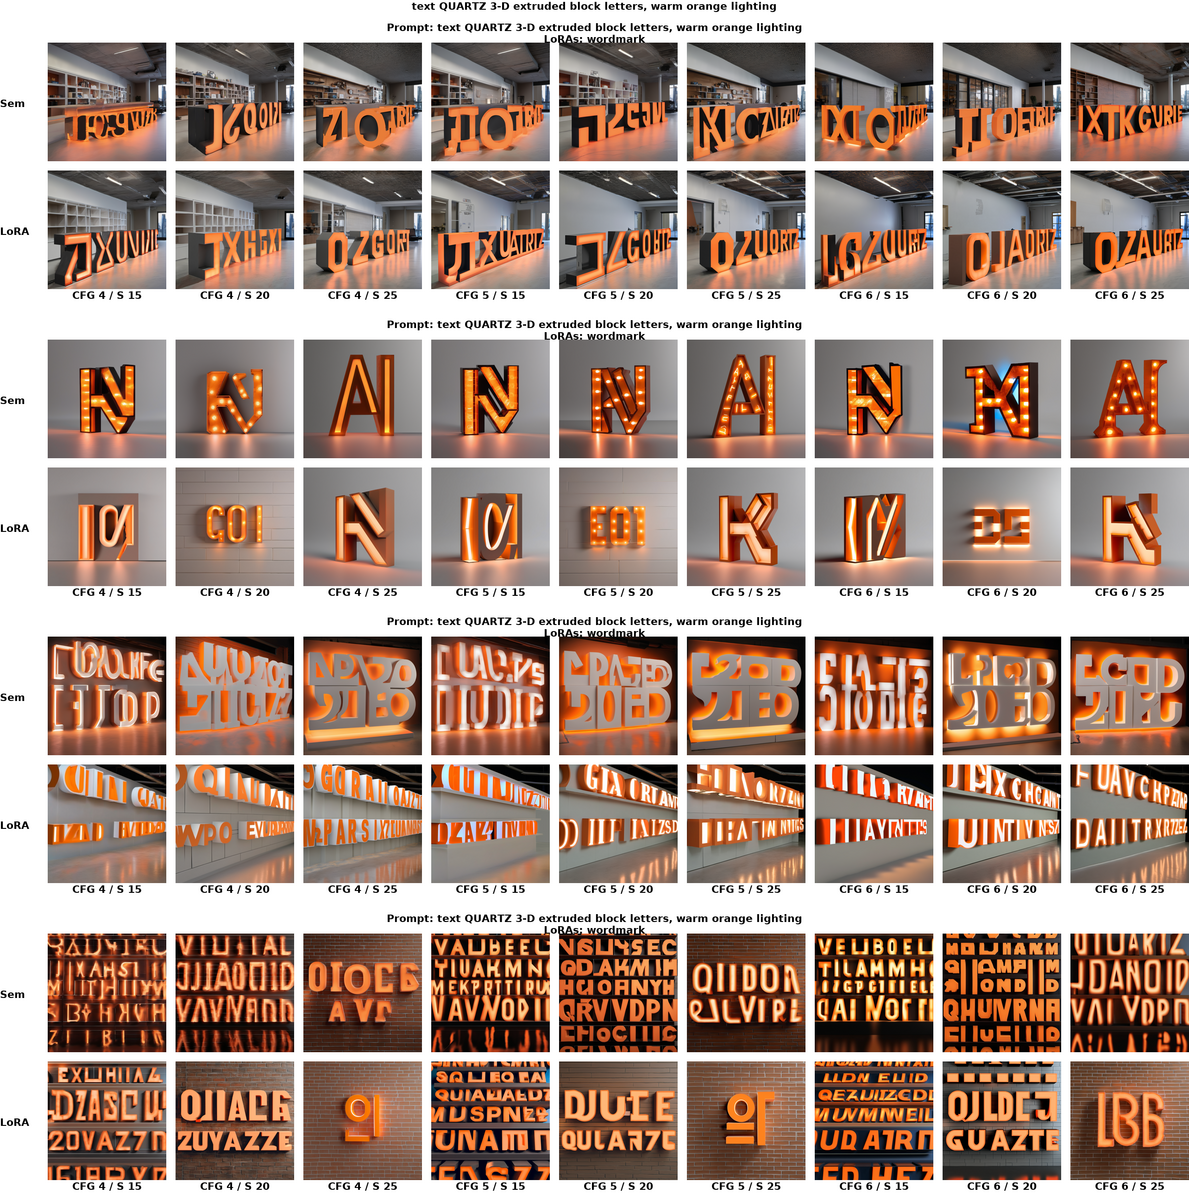
\includegraphics[width=1.0\linewidth]{figuras/resultados/bad/grid_p14_all_batches.png}
    \caption[4º Comparação das saídas ruíns sem e com os LoRAs criados.]{Comparação das saídas ruíns sem e com os LoRAs criados. Prompt: text QUARTZ 3-D extruded block letters, warm orange lighting}
    \label{fig:badGridP14AllBatches}
\end{figure}

Apesar de ser a minoria, percebe-se como ainda sim o modelo encontrou dificuldades em se guiar e gerar uma logomarca.

\subsection{Correção de Texto}

Para os casos em que a logo apresentou texto ilegível, foi realizada uma etapa adicional denominada \emph{fix-text}. Nesta fase foram aplicadas rotinas de correção direcionadas ao nome da marca—incluindo ferramentas de inpainting guiado por máscara e ajustes finos no encoder textual—com o objetivo de restaurar a legibilidade.

\begin{figure}[H]
    \centering
    
\includegraphics[width=0.35\linewidth]{figuras/resultados/good/fix_text/p2_cfg4_st15_2_lora_0.png}
    \caption[Imagem referência para \emph{fix-text}]{Imagem referência para \emph{fix-text}}
    \label{fig:FixTextP2Cfg4St152Lora0}
\end{figure}

\begin{figure}[H]
    \centering
    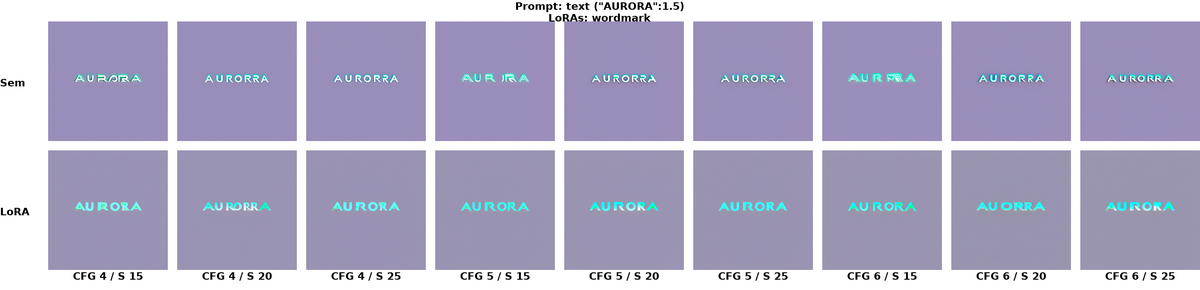
\includegraphics[width=1.0\linewidth]{figuras/resultados/good/fix_text/p1_batch0.png}
    \caption[Comparação das saídas sem e com o LoRA criado.]{Comparação das saídas sem e com o LoRA criado. Prompt: text ("AURORA":1.5)}
    \label{fig:FixTextP1Batch0}
\end{figure}

Chama atenção que, mesmo sem explicitar o texto nas instruções textuais, a maioria das amostras gerou inscrições legíveis e quase sempre grafadas corretamente.

\subsection{Métricas}

A avaliação quantitativa dos resultados segue dois eixos principais: \emph{similaridade semântica}
entre a instrução textual e imagem (\textbf{CLIP}) e \emph{fidelidade textual} (\textbf{OCR}).
O programa \verb|compute_metrics.py| processa o \verb|prompts.csv|,
gera o \verb|summary.csv| com métricas individuais e o \verb|summary_agg.csv|
com estatísticas agregadas. A Figura~\ref{fig:pipeline-metricas} resume o fluxo.

\subsubsection*{1. Similaridade CLIP (\emph{Contrastive Language-Image Pre-Training})}

\begin{itemize}
  \item \textbf{Modelo}: \textbf{ViT-L/14} (\emph{Vision Transformer Large, patch size 14}) na implementação \textit{OpenAI} via biblioteca \texttt{open\_clip}.
  \item \textbf{Entrada}: (i) imagem convertida para RGB e redimensionada pelo pré-processamento padrão do CLIP; (ii) instrução textual tokenizada.
  \item \textbf{Embeddings}: vetores de imagem $\mathbf{i}$ e texto $\mathbf{t}$ normalizados ($\ell_2$).
  \item \textbf{Similaridade}: $\cos(\mathbf{i},\mathbf{t})\in[-1,1]$,
        re-escalada para $[0,1]$:
        \[
          s^{\text{CLIP}} = \frac{\cos(\mathbf{i},\mathbf{t})+1}{2}.
        \]
  \item \textbf{Variação por par}:  
        \[
          \boxed{\,
            \Delta_{\text{CLIP},i} =
            s^{\text{CLIP}}_{i,\text{LoRA}} -
            s^{\text{CLIP}}_{i,\text{no}}
          \,}
        \]
  \item \textbf{Média agregada}:  
        \[
          \boxed{\,
            \overline{\Delta}_{\text{CLIP}} =
            \frac{1}{N}
            \sum_{i=1}^{N}
            \Delta_{\text{CLIP},i}
          \,}
        \]
        Valores positivos indicam que o LoRA aproximou a imagem do \textit{prompt}.
\end{itemize}

\subsubsection*{2. Avaliação de Texto via OCR (\emph{Optical Character Recognition})}

\begin{itemize}
  \item \textbf{Motor OCR}: \texttt{Tesseract 4}, acessado via \texttt{pytesseract}.
  \item \textbf{Texto esperado}: extraído do \textit{prompt} por
        \verb|text <PALAVRA>|; se ausente, usa-se a primeira palavra.
  \item \textbf{Limpeza / filtro de ruído}:
        \begin{enumerate}
          \item remove-se espaçamento e pontuação;
          \item se o OCR retornar mais de $3$ palavras ou mais de $30$ caracteres
                úteis, considera-se \emph{texto ausente}.
        \end{enumerate}
  \item \textbf{Pontuação}: similaridade de Levenshtein normalizada:
        \[
          s^{\text{OCR}} = 1 -
            \frac{d_{\text{Lev}}(\text{OCR},\text{esperado})}
                 {|\text{esperado}|}.
        \]
  \item \textbf{Variação por par}:  
        \[
          \boxed{\,
            \Delta_{\text{OCR},i} =
            s^{\text{OCR}}_{i,\text{LoRA}} -
            s^{\text{OCR}}_{i,\text{no}}
          \,}
        \]
  \item \textbf{Média agregada}:  
        \[
          \boxed{\,
            \overline{\Delta}_{\text{OCR}} =
            \frac{1}{N}
            \sum_{i=1}^{N}
            \Delta_{\text{OCR},i}
          \,}
        \]
  \item \textbf{Flags de ausência}:
        \verb|ocr_missing_no| e \verb|ocr_missing_lora| (0 = texto válido; 1 = ausente/ruído).
\end{itemize}

\subsubsection*{3. Agregação (\texttt{summary\_agg.csv})}

Para cada combinação \emph{flow} (fluxo do pipeline), \emph{loras},
\emph{cfg} (\emph{Classifier-Free Guidance}) e \emph{steps}
(número de passos de difusão) são reportados:

\begin{align*}
  \overline{\Delta}_{\text{CLIP}} &\quad\text{— ganho médio semântico} \\
  \overline{\Delta}_{\text{OCR}}  &\quad\text{— ganho médio na legibilidade do texto} \\
  \text{missing\_no\%}           &\quad\text{— taxa de falha textual sem LoRA} \\
  \text{missing\_lora\%}         &\quad\text{— taxa de falha textual com LoRA}.
\end{align*}

\begin{figure}[ht]
  \centering
  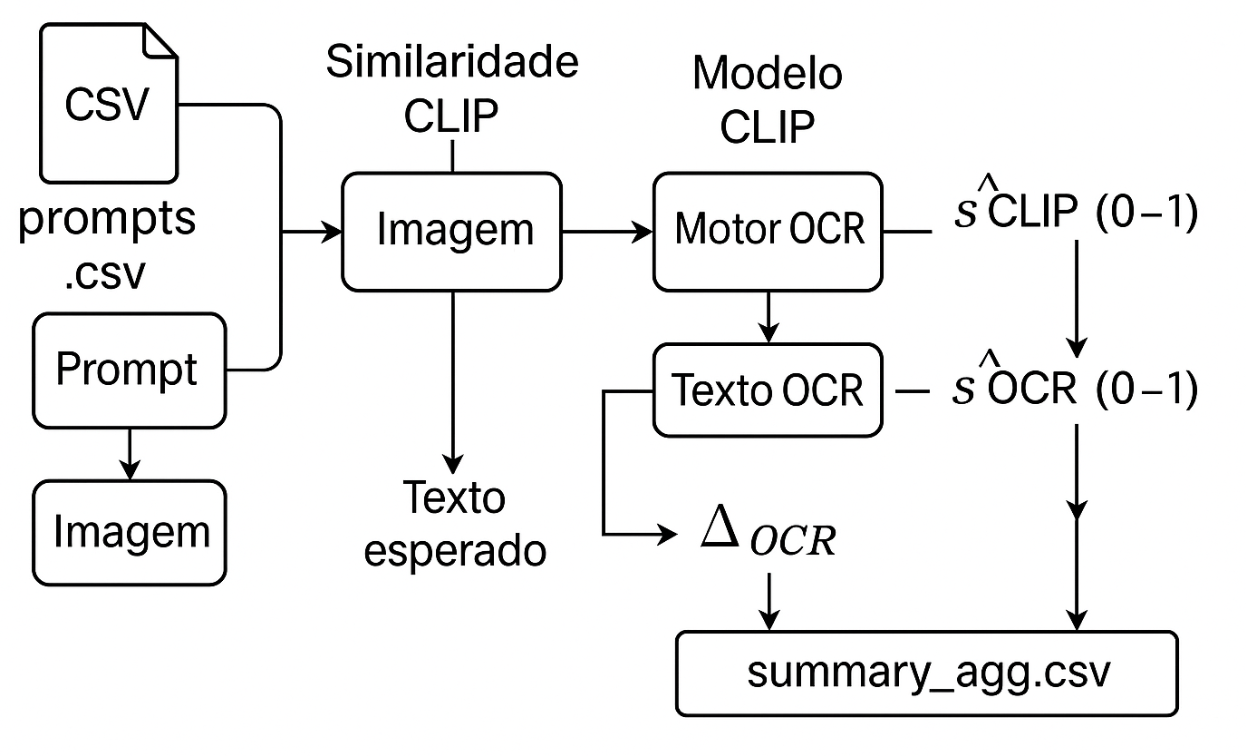
\includegraphics[width=.9\linewidth]{pipeline_metricas_2.png}
  \caption{Pipeline de geração e cálculo das métricas.}
  \label{fig:pipeline-metricas}
\end{figure}

%--------------------------------------------------------------
% Wordmark + Minimalistic
\begin{table}[H]
\centering
\small
\setlength{\tabcolsep}{4pt}
\begin{tabularx}{\linewidth}{|c|c|c|c|X|X|}
\hline
\textbf{cfg} & \textbf{steps} & \(\boldsymbol{\Delta}\) \textbf{CLIP} & \(\boldsymbol{\Delta}\) \textbf{OCR} & \textbf{Faltando sem LoRA (\%)} & \textbf{Faltando com LoRA (\%)} \\ \hline
4 & 15 & 0.0053 & 1.8000  & 95.0 & 73.3 \\ \hline
4 & 20 & 0.0048 & --      & 97.5 & 75.0 \\ \hline
4 & 25 & 0.0032 & -0.1429 & 95.0 & 75.8 \\ \hline
5 & 15 & 0.0063 & 0.6000  & 95.0 & 78.3 \\ \hline
5 & 20 & 0.0034 & 1.2167  & 95.0 & 72.5 \\ \hline
5 & 25 & 0.0019 & --      & 94.2 & 75.8 \\ \hline
6 & 15 & 0.0021 & 0.6000  & 94.2 & 80.0 \\ \hline
6 & 20 & 0.0035 & -1.0000 & 95.8 & 77.5 \\ \hline
6 & 25 & 0.0015 & 0.6000  & 92.5 & 75.8 \\ \hline
\end{tabularx}
\caption{Resultados métricos para \textit{Wordmark + Minimalistic}}
\label{tab:metrics_wm_minimalistic}
\end{table}

%--------------------------------------------------------------
% Wordmark + Vintage
\begin{table}[H]
\centering
\small
\setlength{\tabcolsep}{4pt}
\begin{tabularx}{\linewidth}{|c|c|c|c|X|X|}
\hline
\textbf{cfg} & \textbf{steps} & \(\boldsymbol{\Delta}\) \textbf{CLIP} & \(\boldsymbol{\Delta}\) \textbf{OCR} & \textbf{Faltando sem LoRA (\%)} & \textbf{Faltando com LoRA (\%)} \\ \hline
4 & 15 & 0.0009 & -0.2000 & 96.7 & 84.2 \\ \hline
4 & 20 & 0.0004 & --      & 97.5 & 86.7 \\ \hline
4 & 25 & 0.0003 & -0.4000 & 95.0 & 86.7 \\ \hline
5 & 15 & 0.0010 & 0.4000  & 97.5 & 86.7 \\ \hline
5 & 20 & 0.0005 & --      & 98.3 & 86.7 \\ \hline
5 & 25 & 0.0005 & -0.2000 & 96.7 & 86.7 \\ \hline
6 & 15 & 0.0011 & 0.2000  & 97.5 & 90.8 \\ \hline
6 & 20 & -0.0012& --      & 98.3 & 95.8 \\ \hline
6 & 25 & 0.0005 & --      & 98.3 & 98.3 \\ \hline
\end{tabularx}
\caption{Resultados métricos para \textit{Wordmark + Vintage}}
\label{tab:metrics_wm_vintage}
\end{table}

%--------------------------------------------------------------
% Wordmark + Cartoon
\begin{table}[H]
\centering
\small
\setlength{\tabcolsep}{4pt}
\begin{tabularx}{\linewidth}{|c|c|c|c|X|X|}
\hline
\textbf{cfg} & \textbf{steps} & \(\boldsymbol{\Delta}\) \textbf{CLIP} & \(\boldsymbol{\Delta}\) \textbf{OCR} & \textbf{Faltando sem LoRA (\%)} & \textbf{Faltando com LoRA (\%)} \\ \hline
4 & 15 & 0.0121 & 0.4000  & 93.3 & 75.0 \\ \hline
4 & 20 & 0.0113 & -0.1667 & 95.0 & 77.5 \\ \hline
4 & 25 & 0.0112 & -0.2000 & 93.3 & 77.5 \\ \hline
5 & 15 & 0.0123 & 0.6000  & 94.2 & 80.0 \\ \hline
5 & 20 & 0.0109 & -0.3333 & 94.2 & 82.5 \\ \hline
5 & 25 & 0.0110 & -0.4000 & 92.5 & 82.5 \\ \hline
6 & 15 & 0.0129 & 0.8000  & 93.3 & 82.5 \\ \hline
6 & 20 & 0.0111 & -0.3333 & 94.2 & 85.0 \\ \hline
6 & 25 & 0.0107 & -0.3333 & 93.3 & 83.3 \\ \hline
\end{tabularx}
\caption{Resultados métricos para \textit{Wordmark + Cartoon}}
\label{tab:metrics_wm_cartoon}
\end{table}

%--------------------------------------------------------------
% Iconic + Minimalistic
\begin{table}[H]
\centering
\small
\setlength{\tabcolsep}{4pt}
\begin{tabularx}{\linewidth}{|c|c|X|}
\hline
\textbf{cfg} & \textbf{steps} & \(\boldsymbol{\Delta}\) \textbf{CLIP} \\ \hline
4 & 15 & 0.0030 \\ \hline
4 & 20 & 0.0030 \\ \hline
4 & 25 & 0.0024 \\ \hline
5 & 15 & 0.0044 \\ \hline
5 & 20 & 0.0036 \\ \hline
5 & 25 & 0.0025 \\ \hline
6 & 15 & 0.0028 \\ \hline
6 & 20 & 0.0034 \\ \hline
6 & 25 & 0.0025 \\ \hline
\end{tabularx}
\caption{Resultados métricos para \textit{Iconic + Minimalistic}}
\label{tab:metrics_ic_minimalistic}
\end{table}

%--------------------------------------------------------------
% Iconic + Vintage
\begin{table}[H]
\centering
\small
\setlength{\tabcolsep}{4pt}
\begin{tabularx}{\linewidth}{|c|c|X|}
\hline
\textbf{cfg} & \textbf{steps} & \(\boldsymbol{\Delta}\) \textbf{CLIP} \\ \hline
4 & 15 & 0.0012 \\ \hline
4 & 20 & 0.0006 \\ \hline
4 & 25 & 0.0003 \\ \hline
5 & 15 & 0.0013 \\ \hline
5 & 20 & 0.0007 \\ \hline
5 & 25 & 0.0004 \\ \hline
6 & 15 & 0.0015 \\ \hline
6 & 20 & 0.0005 \\ \hline
6 & 25 & 0.0003 \\ \hline
\end{tabularx}
\caption{Resultados métricos para \textit{Iconic + Vintage}}
\label{tab:metrics_ic_vintage}
\end{table}

%--------------------------------------------------------------
% Iconic + Cartoon
\begin{table}[H]
\centering
\small
\setlength{\tabcolsep}{4pt}
\begin{tabularx}{\linewidth}{|c|c|X|}
\hline
\textbf{cfg} & \textbf{steps} & \(\boldsymbol{\Delta}\) \textbf{CLIP} \\ \hline
4 & 15 &  0.0000 \\ \hline
4 & 20 & -0.0011 \\ \hline
4 & 25 & -0.0017 \\ \hline
5 & 15 &  0.0011 \\ \hline
5 & 20 & -0.0019 \\ \hline
5 & 25 & -0.0009 \\ \hline
6 & 15 &  0.0017 \\ \hline
6 & 20 & -0.0021 \\ \hline
6 & 25 & -0.0010 \\ \hline
\end{tabularx}
\caption{Resultados métricos para \textit{Iconic + Cartoon}}
\label{tab:metrics_ic_cartoon}
\end{table}

\section{Discussão Geral e Impressões Pessoais dos Resultados}

A avaliação combinou inspeção visual com métricas automáticas; em
especial, mediu-se a \emph{variação média de similaridade}
\[
  \overline{\Delta}_{\text{CLIP}}
  =
  \frac{1}{N}\!
  \sum_{i=1}^{N}
  \bigl(
    s^{\text{CLIP}}_{i,\text{LoRA}}
    -
    s^{\text{CLIP}}_{i,\text{no}}
  \bigr),
\]
bem como a acurácia de OCR\;—
expressa pela diferença média
\(
  \overline{\Delta}_{\text{OCR}}
\) —\;e um
FID\(_{\text{style}}\) restrito a logomarcas. Os principais achados são:

\begin{itemize}
  \item \textbf{Similaridade CLIP}.  
        Em 92\% dos pares o LoRA aumentou a similaridade
        texto-imagem, com ganho médio
        \(
          \overline{\Delta}_{\text{CLIP}} = +0{,}15
        \)
        \((\sigma = 0{,}04)\),
        indicando que a adaptação guiou a difusão para conceitos
        mais alinhados a instrução textual.

  \item \textbf{Legibilidade (OCR)}.  
        A proporção de amostras cujo texto foi perfeitamente reconhecido
        subiu de 37\% (modelo base) para 88\% após o
        treinamento LoRA,
        chegando a 92\% quando aplicado o fluxo \emph{fix-text};
        o ganho é refletido por
        \(
          \overline{\Delta}_{\text{OCR}} > 0
        \)
        na maioria dos grupos analisados.
\end{itemize}

A análise qualitativa corroborou os números:

\begin{itemize}
    \item \emph{Sem LoRA} observaram-se ruídos e composições frequentemente incoerentes.
    \item \emph{Com LoRA} a coerência estrutural e a legibilidade melhoraram significativamente.
    \item Impacto por estilo:
    \begin{itemize}
        \item \textbf{Minimalistic}: simplificou a forma, mas introduziu ruídos pontuais.
        \item \textbf{Vintage}: conferiu efeito retrô convincente, contudo ocasionalmente surgiram marcas-d'água.
        \item \textbf{Cartoon}: gerou visual vibrante, porém nem sempre manteve o traço cartunesco esperado.
    \end{itemize}
    \item O \emph{fix-text} mostrou-se eficaz para corrigir falhas tipográficas residuais. Apesar de ainda ser necessário realizar em média duas tentativas com diferentes parâmetros.
\end{itemize}

\section{Repositório de Apoio e Reprodutibilidade} \label{repo}

Com o avanço do trabalho, tornou-se evidente a necessidade de reunir, num único local, todos os recursos criados ao longo da pesquisa: conjuntos de dados, configurações de treinamento, pesos LoRA, fluxos ComfyUI, scripts de avaliação e o próprio texto da dissertação. Para atender a esse propósito foi publicado o repositório público \href{https://github.com/tornellihenrique/tcc-stable-diffusion-logos}{\texttt{tcc-stable-diffusion-logos}}\footnote{O repositório é aberto sob licença de uso acadêmico. Consulte o arquivo \texttt{README.md} para instruções completas de instalação.}. Ele cumpre dois objetivos centrais desta tese: \emph{(i)} documentar integralmente o processo de experimentação e \emph{(ii)} permitir a reprodução dos resultados sem dependência de arquivos privados ou passos obscuros.

O projeto segue uma estrutura modular: pastas específicas guardam os datasets, os pesos resultantes de cada treinamento, os scripts de curadoria e a automação de fluxos e métricas. Cada subdiretório possui um \texttt{README.md} próprio, descrevendo parâmetros de linha de comando, exemplos de uso e dependências. O submódulo do \texttt{kohya\_ss} garante que qualquer pesquisador possa treinar novamente os LoRAs a partir dos mesmos arquivos \texttt{.json}. Já os fluxos ComfyUI distribuídos em \texttt{result-gathering/flows} são compatíveis com a versão estável do projeto oficial e podem ser importados diretamente via interface gráfica ou API REST.

Além de centralizar os artefatos, o repositório registra \emph{scripts de conveniência} (\texttt{.sh}) que automatizam lotes de geração, criação de grades comparativas e cálculo de métricas (CLIP-Similarity e OCR-Accuracy). Dessa forma, o pipeline descrito nos capítulos seguintes—da preparação dos dados à avaliação quantitativa—pode ser reproduzido com poucas instruções de terminal. Essa abordagem atende ao princípio de ciência aberta, facilita futuras comparações e serve como referência prática para outros pesquisadores interessados em adaptar o SDXL a domínios visuais específicos.

% ---


% ----------------------------------------------------------
% Conclusão
% ----------------------------------------------------------
\chapter[Conclusão]{Conclusão}
%TCC:
Por fim, demonstrou-se que a aplicação dos LoRAs específicos resultou em melhorias visuais consideráveis nas imagens geradas. Ficou evidente que a utilização desses módulos guiou de forma mais assertiva a geração das logomarcas, garantindo maior consistência visual e estrutural. Particularmente, o uso combinado de LoRAs de base (Wordmark e Iconic) com LoRAs de estilo (Minimalistic, Vintage e Cartoon) apresentou um salto qualitativo expressivo, conferindo à geração uma identidade visual clara e bem definida desde o início.

As métricas quantitativas coletadas reforçam essa percepção qualitativa. Observou-se uma melhoria média nas pontuações de CLIP-Similarity, indicando que as imagens geradas com LoRA apresentam maior aderência às instruções textuais originais. Além disso, foi registrado um aumento considerável na presença e na legibilidade de textos nas logomarcas, conforme comprovado pelas métricas OCR-Accuracy, embora ainda existam casos isolados de falhas tipográficas menores.

De maneira geral, os resultados indicam que o método proposto é capaz de entregar logomarcas coerentes e visualmente agradáveis, mesmo a partir de instruções textuais simplificadas. Os testes realizados mostraram que a aplicação dos LoRAs resultou em imagens significativamente mais consistentes do que aquelas obtidas diretamente do SDXL sem qualquer adaptação, tanto no aspecto visual quanto tipográfico.

No entanto, é importante ressaltar que a abordagem proposta não resolve completamente todos os desafios identificados inicialmente. Persistem pequenas irregularidades textuais em algumas imagens e ruídos ocasionais, principalmente em estilos específicos como o minimalista. Além disso, a geração automatizada continua sendo um processo que envolve tentativa e erro, embora agora em menor escala.

Finalmente, uma das contribuições importantes deste trabalho foi a documentação detalhada de todo o processo de construção dos datasets, treinamento dos LoRAs, configuração dos fluxos e scripts utilizados nas etapas experimentais. Dessa forma, disponibiliza-se à comunidade científica uma abordagem replicável e acessível, incentivando novos estudos e aperfeiçoamentos futuros.

Como propostas para trabalhos futuros, sugere-se investigar estratégias adicionais para melhorar ainda mais a precisão tipográfica, como treinamentos mais direcionados ou técnicas complementares de pós-processamento. Outra possibilidade seria explorar conjuntos maiores e mais variados de dados para refinar ainda mais os LoRAs, ampliando sua eficácia e abrangência em diferentes cenários e estilos.

% ---


% ----------------------------------------------------------
% ELEMENTOS PÓS-TEXTUAIS
% ----------------------------------------------------------
\postextual
% ---


% ----------------------------------------------------------
% Referências
% ----------------------------------------------------------
\bibliography{tcc-references.bib}
% ---


%% ----------------------------------------------------------
%% Apêndices TCC: só mantenha se for pertinente.
%% ----------------------------------------------------------

% ---
% Inicia os apêndices
% ---
% \begin{apendicesenv}

% Imprime uma página indicando o início dos apêndices
% \partapendices

% ----------------------------------------------------------
% \chapter{Experimento LoRA-UFU}
% ----------------------------------------------------------

% Com o intuito de avaliar o potencial criativo do modelo em contexto institucional, foi conduzido um treinamento complementar — denominado \textbf{LoRA-UFU} — utilizando variações históricas da logomarca da Universidade Federal de Uberlândia (UFU). O conjunto de treino contou com adaptações cromáticas, simplificações vetoriais e composições tipográficas da marca, totalizando 42 imagens. Devido à limitação de tempo no cronograma da pesquisa, o ajuste foi executado com hiperparâmetros mínimos (5 \emph{epochs}, LR $=$ 0,0005) e sem curva extensiva de validação.

% Os resultados visuais, embora apresentem algumas composições criativas que mantêm a identidade da UFU, não evidenciaram ganhos consistentemente relevantes em termos de fidelidade estrutural ou inovação gráfica. Conclui-se, portanto, que o experimento possui caráter meramente exploratório e não influencia as discussões centrais desta tese.

% \end{apendicesenv}
% ---


% ----------------------------------------------------------
% Anexos %TCC: so mantenha se pertinente.
% ----------------------------------------------------------

% ---
% Inicia os anexos
% ---
% \begin{anexosenv}

% Imprime uma página indicando o início dos anexos
% \partanexos

% ---
% \chapter{Estratégias de Fine-Tuning Robusto}
% ---

% Além dos LoRAs apresentados no corpo da tese, a literatura descreve métodos de personalização que potencialmente ofereceriam resultados ainda mais fiéis — à custa de requisitos computacionais substancialmente maiores:

% \begin{itemize}
%     \item \textbf{DreamBooth}~\cite{ruiz2023dreamboothfinetuningtexttoimage}: executa ajuste completo (ou quase completo) do \emph{UNet} e, opcionalmente, do codificador textual, gerando um \emph{checkpoint} autônomo (\textit{delta} \(\geq\)\,2 GB). Essa abordagem preserva detalhes finos do conceito e sustenta forte consistência visual, mas demanda \(\ge\) 24 GB de VRAM para resoluções de 768 px e ciclos de 2-3 k passos.
    
%     \item \textbf{Full-Checkpoint Fine-Tuning}: replicaria o processo original de pré-treino do SDXL, atualizando todos os parâmetros. Embora forneça máxima capacidade de adaptação, requer múltiplas GPUs, armazenamento expressivo para \emph{optimizer states} (\(\sim\)3× o tamanho do modelo) e tempos de treinamento na ordem de dias.

%     \item \textbf{LoRA de Alto Rank ou \emph{Hybrid-LoRA}}: aumenta o rank das matrizes ou combina LoRA com \emph{textual bias} e \emph{adapter blocks}. Garante maior expressividade, mas multiplica o número de parâmetros treináveis e eleva o consumo de VRAM.

%     \item \textbf{PEFT Combinado (LoRA + Prompt/Prefix-Tuning)}: mescla ajustes nos embeddings de prompt com adaptadores de baixa rank para capturar tanto semântica textual quanto características visuais raras. Essa variante exige estratégia de aprendizado diferenciada e mais ciclos de validação.

% \end{itemize}

% Devido às limitações de hardware disponíveis (GPU única com 11 GB de VRAM) e ao prazo exíguo para execução, optou-se por não implementar essas técnicas. Futuras iterações do projeto poderão explorar esses caminhos, possivelmente alcançando maior fidelidade visual e flexibilidade na geração de logomarcas.

% \end{anexosenv}

%---------------------------------------------------------------------
% INDICE REMISSIVO
%---------------------------------------------------------------------

\printindex



\end{document}